% Template authors: Bogumił Kamiński and Michał Jakubczyk

\documentclass[12pt,a4paper,twoside,openany]{book}
\usepackage[T1]{fontenc}
\usepackage[utf8]{inputenc}
\usepackage[polish]{babel}
\usepackage{graphicx}
\usepackage{times}
\usepackage{indentfirst}
\usepackage[left=3cm,right=2cm,top=2.5cm,bottom=2.5cm]{geometry}
\usepackage{natbib}

\usepackage{enumitem}
\usepackage{color}
\usepackage{soul}
\usepackage{tikz}
\usepackage{url}
\usepackage{todonotes}
\usepackage{verbatim}

% --- package for automatic insertion of R code -----------------------
\usepackage{listings}
\lstset{language=R,%
   numbers=left,%
   tabsize=3,%
   numberstyle=\footnotesize,%
   basicstyle=\ttfamily \scriptsize \color{black},%
   escapeinside={(*@}{@*)}}

%dodane przeze mnie
\usepackage{float}
\usepackage{subcaption}
\captionsetup{compatibility=false}


\usepackage{algorithmic,algorithm}
\usepackage{amsmath}
\DeclareMathOperator*{\argmin}{argmin}
\DeclareMathOperator*{\argmax}{argmax}
\newcommand*{\argminl}{\argmin\limits}
\newcommand*{\argmaxl}{\argmax\limits}
\usepackage{makecell}
%

\setlist{itemsep=0pt}
\setlist{nolistsep}
\frenchspacing
\linespread{1.3}
\addto\captionspolish{%
\renewcommand*\listtablename{Spis tabel}
\renewcommand*\tablename{Tabela}
}
\usepackage{titlesec}
\titlelabel{\thetitle.\quad}

\frenchspacing

\begin{document}

\begin{center}

\includegraphics[scale=0.3]{logo.JPG}

\vspace{1cm}

% tu i dalej fbox należy usunąć i wpisać odpowiednią wartość
Studium magisterskie
\end{center}

\vspace{1cm}

\noindent Kierunek: Metody ilościowe w~ekonomii i~systemy informacyjne

%\noindent Specjalność: \fbox{\vphantom{I}\dots}

\vspace{1cm}

{
\leftskip=10cm\noindent
Michał Cisek\newline
Nr albumu: 56283

}

\vspace{2cm}

\title{Prognoza kierunku cen akcji za pomocą \\metod klasyfikacji kombinowanej}

\makeatletter

\begin{center}
\LARGE\bf
\@title
\end{center}

\vspace{2cm}

{
\leftskip=10cm\noindent
Praca magisterska\newline 
napisana w~Instytucie Ekonometrii\newline
pod kierunkiem naukowym\newline
dr.~Michała Jakubczyka

}

\vfill

\begin{center}
Warszawa, \the\year
\end{center}
\thispagestyle{empty}

\clearpage
\thispagestyle{empty}
\mbox{}
% druga strona będzie pusta, ponieważ drukujemy dwustronnie
% a mbox jest po to, żeby ta strona się pokazała
% od procenta robimy komentarze
\clearpage

\tableofcontents

\clearpage

\chapter{Wprowadzenie}

Tematykę predykcji cen spółek poruszało na przestrzeni lat wielu badaczy \citep[np.][]{almanza2006,xu2014,ferreira2008,rajput2016}. Szczególna charakterystyka finansowych szeregów czasowych powoduje, że stosowanie prostych, jak i specjalizowanych metod statystycznych do szeregów czasowych nie przynosi wymiernych korzyści \citep{kwiatkowski1992}. Na przestrzeni lat pojawiało się wiele propozycji przezwyciężenia trudności modelowania danych finansowych. Do problemów z niestacjonarnością cen i autokorelacją stóp zwrotu proponowane są modele takie jak ARIMA \citep{adebiyi2014,bontempi2012}, natomiast do występujących efektów grupowania wariancji popularne w zastosowaniu są modele klasy GARCH, por.~np.~\citet{zhang2009} i \citet{arowolo2013}. Oba wspomniane modele, mimo wprowadzenia wielu modyfikacji i usprawnień \citep{jiang2012}, nie potrafiły w pełni uchwycić natury rynków finansowych \citep{degooijer2006}. 

Celem niniejszej pracy jest poprawa skuteczności predykcji kierunku cen akcji notowanych na Giełdzie Papierów Wartościowych w Warszawie za pomocą metod klasyfikacji kombinowanej (ang.~\textit{ensembling learning}). Rola rynku kapitałowego w życiu gospodarki jest niepodważalna. Szacuje się, że w 2013 roku w Polsce, łączna wielkość przychodów przedsiębiorstw notowanych na głównym parkiecie wynosiła 536 mld zł, co stanowiło ok. 14\% przychodów przedsiębiorstw niefinansowych. Ponadto zestawiając ze sobą fakt istnienia 19 tys. firm zatrudniających powyżej 50 osób, oraz potencjał około 900 polskich spółek do debiutu giełdowego (\url{goo.gl/vvkNbu}), widać jak duży potencjał jest obecny na polskich rynku kapitałowym. Problem prognozwania kierunku zmiany kwotowań jest szczególnie istotny z punktu widzenia instytucji finansowych oraz inwestorów instytucjonalnych. Szacuje się, że w Stanach Zjednoczonych około 73\% obrotu na rynku kapitałowym pochodzi z handlu algorytmicznego \citep{mackenzie2009}, czyli handlu, w którym to komputer podejmuje decyzję kupna bądź sprzedaży na podstawie wcześniej zdefiniowanego algorytmu. Poprawa skuteczności predykcji takich algorytmów nawet o kilka procent może przekładać się na znaczący wzrost zysków banków inwestycyjnych czy pojedynczych inwestorów. Dlatego też istotne jest pokazanie klasyfikacji kombinowanej jako narzędzia, pozwalającego na poprawę skuteczności predykcji, a jednocześnie zmniejszającego ryzyko zbytniego dopasowania do danych. Dodatkowym celem będzie zweryfikowanie hipotezy rynku efektywnego. Hipoteza ta zakłada że pojawienie się informacji na rynku prowadzi do natychmiastowego jej odzwierciedlenia w cenie instrumentu finansowego \citep{basu1977}. Szczegółowiej, rynek można określić jako efektywny w przypadku spełnienia szeregu założeń. Do tych postulatów można zaliczyć między innymi bezpłatność informacji, równą ich dostępność dla wszystkich uczestników rynku, czy brak kosztów transakcyjnych. Istnieją trzy wersje hipotezy: słaba, półsilna i silna. Każda z nich zakłada niemożliwość osiągnięcia ponadprzeciętnych zysków poprzez używanie metod analizy technicznej. Półsilna zaprzecza użyteczności analizy fundamentalnej, a silna wyklucza nawet insider trading, jako możliwy sposób na „pokonanie” rynku. Zatem, jeśli hipoteza rynku efektywnego jest spełniona, ceny powinny zachowywać się jak biały szum i nie dać w żaden sposób się przewidzieć na podstawie historycznych danych. 

Na przestrzeni ostatnich lat często używaną techniką uczenia maszynowego w przewidywaniu cen spółek są sztuczne sieci neuronowe \citep[np.][]{sureshkumar2011,kara2011,mohan2005,moghaddam2016}. Naśladują one budowę naturalnych neuronów i zbudowane są z wzajemnie połączonych węzłów, ułożonych w kolejnych warstwach. Sieci neuronowe przypisują wagi poszczególnym połączeniom, tak że wynik obliczony jest na ich podstawie oraz danych wejściowych. Wraz z przebiegiem kolejnych iteracji algorytm rozpoznaje wzorce ukryte w danych i przypisuje na nowo wagi połączeniom między warstwami. Badania dowiodły skutecznoci nieznacznie powyżej 50\% dla rzeczywistych danych notowanych spółek, z wyjątkiem sytuacji występowania zwiększonej wariancji w danych \citep{patel2014}. Jak zostało wspomniane wcześniej, i takie zjawisko obecne jest w finansowych szeregach czasowych. Kolejnym przykładem są sieci SVM. Używają one tzw. funkcji jądra (ang. kernel functions), które służą do oceny podobieństwa między dwoma obserwacjami. Po określeniu podobieństwa dla całego zbioru danych, algorytm znajduje granicę decyzyjną, która maksymalizuje dystans pomiędzy najbliższymi członkami różnych klas. Wybierając liniową funkcję jądra, SVM staje się algorytmem podobnym do regresji logistycznej, dlatego prawdziwa przewaga ujawnia się dopiero przy zastosowaniu nieliniowych kernelów, które pozwalają na modelowanie nieliniowych granic decyzyjnych. Przydatność sieci wektorów nośnych została udowodniona w wielu artyukułach \citep[np.][]{thenmozhi2016,shen2015}, a skuteczność w predykcji kierunku przyszłych cen akcji została wykazana na poziomie nawet 57\% \citep{kim2003}. Słabymi stronami tego algorytmu jest duża złożoność obliczeniowa i trudność w odpowiedniej parametryzacji ze względu na mnogość dostępnych funkcji jądra i skutków jakie niesie ze sobą wybór jednej względem innej. Jeśli chodzi o hipotezę rynku efektywnego, zostało wykazane występowanie zjawisk, które jej przeczą. Przykładowo, ceny akcji które w ostatnim czasie rosły przejawiają tendencje do kolejnych wzrostów, a spadki pociągają za sobą statystycznie częściej kolejne spadki \citep{jegadeesh1993}. To nakłada na finansowe dane swego rodzaju przewidywalność, przeciwnie do tego co stwierdza hipoteza rynku efektywnego. Dodatkowo rynek akcji doświadcza występowania trendów sezonowych, tzn. wysokich zwrotów w okresie zimowym i niskich w okresie letnim \citep{jacobsen2013,granger1992}. Ponadto znane jest występowaniu pewnych anomalii rynkowych \citep{bouman2002}, takich jak efekt stycznia czy rajd św. Mikołaja (zwany także efektem grudnia). 

Dane użyte w pracy zawierają notowania spółek notowanych na Giełdzie Papierów Wartościowych w Warszawie od momentu pierwszego kwotowania, czyli 16 kwietnia 1991 r. Ze względu jednak na ograniczoną płynność przez pierwsze lata funkcjonowania giełdy, oraz niską zmienność i podatność na manipulacje cen niektórych spółek, końcowy zbiór danych został ograniczony tylko do przedsiębiorstw wchodzących w skład 20 największych spółek notowanych na GPW (WIG20) na dzień 10 marca 2017.  Zmienną objaśnianą użytą w pracy jest kierunek, jaki wykonają ceny akcji w różnym horyzoncie czasowym (1, 5, 10, 20, 90, 270 dni). W celu zapewnienia zrównoważonej próby, w przypadku braku zmiany ceny w danym przedziale, kierunek określany jest jako pozytywny. W charakterze zmiennych objaśniających występują wskaźniki określające występujący trend oraz zmienność rynkową, a także wskaźniki analizy technicznej, takie jak RSI, MACD czy CCI. Przydatność tych indykatorów została potwierdzona m.in.~w pracy \citet{wong2003}. Do modelowania zostaną użyte techniki klasyfikacji kombinowanej, takie jak agregacja modeli poprzez uśrednianie bądź głosowanie (ang.~\textit{bagging}), wzmacnianie (ang.~\textit{boosting}), metauczenie (ang.~\textit{meta-learning}) czy kontaminacje modeli (ang.~\textit{stacking}). W przypadku zmniejszenia błędów predykcji na zbiorze testowym w stosunku do pojedynczych klasyfikatorów będziemy mogli stwierdzić, iż techniki łączenia klasyfikatorów lepiej sprawdzają się do omawianego zagadnienia. Dodatkową kwestią będzie zweryfikowanie hipotezy rynku efektywnego na polskim rynku akcji. Jeśli hipoteza okaże się prawdziwa, wtedy żaden zbiór klasyfikatorów nie będzie miał istotnie większej skuteczności niż 50\% (losowe zgadywanie co do przyszłego kierunku cen). W przeciwnym razie będziemy mogli stwierdzić, że rynek w pewnym stopniu wykazuje nieefektywność, a więc jest możliwość wyciągnia wniosków co do przyszłego kierunku cen akcji na podstawie historycznych obserwacji. 

Praca podzielona jest na 4 rozdziały i dodatkowo zawiera dwa dodatki. Rozdział 1 składa się z dwóch części: pierwsza zawiera wprowadzenie do zagadnienia uczenia maszynowego, opis zadań stawianych przez nią, oraz jej rozwój na przestrzeni ostatnich lat, natomiast druga zawiera teoretyczne aspekty klasyfikatorów użytych w dalszej części pracy. Drugi rozdział zawiera omówienie klasyfikacji kombinowanej, jej matematyczne podstawy oraz opis metod, które wchodzą w jej skład. Na rozdział 3 składa się opis metodologii wykonanych analiz oraz wyniki. Ostatni rozdział zawiera podsumowanie pracy. W dodatku A zamieszczone zostały kody użyte do wygenerowania prezentowanych rezultatów, natomiast na dodatek B składają się dane w postaci relacyjnej bazy danych, zawierające wszystkie notowania spółek z warszawskiego parkietu.

\clearpage

\chapter{Uczenie maszynowe}

Rozdział ten zawiera podstawowe informacje na temat uczenia maszynowego. Zostały przedstawione najważniejsze definicje, a także problemy stawiane przed tą dziedziną. Ponadto opisane są techniczne aspekty algorytmów uczenia maszynowego użytych w dalszej części pracy.

\section{Podstawowe zagadnienia}

W 2001 grupa Gartner opublikowała raport (\url{goo.gl/2ic1P8}), w którym oszacowała coroczny przyrost wytworzonych danych na poziomie 59\%. Zaznaczono przy tym, iż wielkość danych nie jest jedynym problemem. Równie ważna jest różnorodność zbieranych danych (dane w formie tabelarycznej, hierarchicznej, pochodzące z wiadomości e-mail, plików wideo, audio czy transakcji finansowych), a także zmienność (szybka produkcja danych przy jednoczesnej potrzebie szybkiego ich przetworzenia). Charakterystyka ta sprawia, że pojawiają się wyzwania związane z przechwytywaniem, składowaniem, transferem, wizualizacją czy analizą takich zbiorów danych. Według raportu firmy Dell (\url{goo.gl/GtRFYr}) w samych Stanach Zjednoczonych produkcja danych między rokiem 2012 a 2020 wzrośnie z 898 egzabajtów do 6.6 zettabajtów, co oznacza podwojenie wytwarzania danych co 3 lata. Z taką ilością danych wiąże się jednocześnie możliwość wyciągnięcia wiedzy użytecznej w wielu dziedzinach, takich jak zwalczanie przestępczości (\url{goo.gl/HYffTW}), medycyna (\url{goo.gl/uT6kxY}) czy marketing (\url{goo.gl/3xziAi}). Niemniej jednak należy zauważyć, iż obecnie mniej niż 0.5\% zbieranych danych jest analizowana i używana dalej (\url{goo.gl/SwpfcR}). 


\subsection{Definicje}
Zalew danych powoduje, że pożądane są zautomatyzowane metody analizy danych. Dobrym przykładem wykorzystania możliwości big data jest zastosowanie technik uczenia maszynowego (\url{goo.gl/JwJon7}). Uczenie maszynowe (ang.~\textit{machine learning}) jest interdyscyplinarną nauką z pogranicza statystyki, matematyki oraz informatyki, która daje możliwość komputerom nauki bez konieczności jawnego zaprogramowania. Szczegółowiej, uczeniem maszynowym nazywamy zbiór metod, które w sposób zautomatyzowany starają się znaleźć wzorce w danych, by następnie użyć ich do predykcji na nowych zbiorach, bądź też wspomóc inny proces podejmowania decyzji w warunkach niepewności. Nacisk kładziony jest na wysoce skalowalną analitykę predykcyjną, używając metod na tyle uniwersalnych, że pozwalają na uproszczenie niektórych zadań w analizie danych. Uproszczenie to polega na takiej konstrukcji algorytmów uczących, by komputer był w stanie pozyskiwać wiedzę ze zbiorów bez pomocy człowieka. Paradygmat uczenia maszynowego może być postrzegany, jako „programowanie poprzez podawanie przykładów”. Jeśli weźmiemy pod uwagę problem rozpoznawania wiadomości email typu spam, to używając metod machine learning, zamiast rozwiązać to zadanie bezpośrednio, będziemy starali się znaleźć takie metody, które pozwolą komputerowi samemu dojść do rozwiązania na podstawie dostarczonych mu przykładów. Przewagą takiego podejścia nad zastosowaniem do tego celu eksperckiej wiedzy ludzkiej jest możliwość uwzględnienia ilości danych, której żaden człowiek nie byłby samodzielnie w stanie zanalizować oraz odnalezienie tak złożonych zależności między danymi, które byłyby niemożliwe do wykrycia przez ludzkie oko. Ważnym aspektem uczenia maszynowego jest także generalizacja zdobytej wiedzy. Najprostszym rozwiązaniem wspomnianego problemu wiadomości spam byłoby zapamiętanie przez komputer wszystkich wiadomości w zbiorze uczącym (zbiór użyty do wytrenowania algorytmu, w celu zdobycia wiedzy na dany temat) oznaczonych jako spam. W momencie, kiedy przychodziłaby nowa wiadomość, komputer sprawdzałby czy dana wiadomość znajduje się we wcześniej stworzonym zbiorze i w takim przypadku klasyfikował by ją jako wiadomość, zawierającą treści marketingowe, a w przeciwnym razie umieściłby ją w skrzynce odbiorczej. O ile takie podejście uczenia poprzez zapamiętywanie może być czasami użyteczne, o tyle tracimy ważną umiejętność, jaką jest zdolność klasyfikacji wiadomości, które wcześniej nie pojawiły się. Dlatego też ważną cechą skutecznego uczenia jest używanie pojedynczych przykładów do stworzenia jak najbardziej generalnej wiedzy. Aby stworzyć generalizację w przypadku klasyfikacji spamu, algorytm może przeszukać wcześniej oznaczone maile i wyznaczyć z nich kluczowe słowa, które indukują niepożądaną wiadomość. W przypadku otrzymania nowego maila, komputer sprawdzałby czy występuje co najmniej jedno z tych słów i na tej podstawie podjąłby decyzję o przynależności danej wiadomości.

Należy jednak rozgraniczyć pojęcie uczenia maszynowego od eksploracji danych (ang.~\textit{data mining}). Oba te pojęcia oznaczają przeszukiwanie danych pod kątem znalezienia ukrytych wzorców, jednak data mining jest pojęciem węższym, jako że korzysta z technik i podwalin zbudowanych na uczeniu maszynowym. Zazwyczaj celem jest zdobycie jakichś wstępnych spostrzeżeń, co do zbioru danych, o którym wcześniej posiadano niewielką wiedzę. Nie dąży się do posiadania zaawansowanego rozumienia procesu generującego dane, lecz istotne jest zbudowanie intuicji wokół tego, co dzieje się w danych. Z drugiej strony, uczenie maszynowe korzysta z niektórych metod eksploracji danych oraz innych algorytmów uczących, tak żeby odkryć wiedzę ukrytą w danych, ale ponadto jest w stanie dokonywać predykcji na rekordach, które nie zostały użyte do uczenia modelu.


\subsection{Motywacja}
Istotną kwestią jest określenie sytuacji, w których uczenie maszynowe może okazać się dużo bardziej pomocne niż bezpośrednie programowanie konkretnego zadania. W szczególności dwie cechy danego problemu mogą wskazywać na użyteczność technik, które uczą się i poprawiają swoje działanie na podstawie wiedzy zdobytej ze zbioru danych. Pierwszą z nich jest złożoność. Możemy tutaj zaliczyć zadania, które są wykonywane przez człowieka rutynowo, jednak postrzeganie ich przez nas nie jest na tyle rozbudowane, by móc zdefiniować na tej podstawie ustrukturyzowany algorytm. Jako przykłady można tutaj podać rozpoznawanie mowy, postrzeganie (zrozumienie) obrazów czy jazdę samochodem. Okazuje się, że dla wszystkich tych czynności, pod warunkiem dostarczenia odpowiednio dużej ilości informacji treningowej, techniki uczenia maszynowego osiągają zadowalające wyniki \citep[][]{hinton2012,ciregan2012,ajaykumar2016}. Są także zadania, które swoją złożonością przekraczają ludzie możliwości. Mowa tutaj np. o bazie danych genomów ludzkich, danych pogodowych czy danych pochodzących z aukcji internetowych, których wielkość uniemożliwia przeprowadzanie ręcznych analiz danych. Dlatego obiecujące wydaje się użycie uczących się algorytmów do tego typu zadań, gdzie w połączeniu ze stale rosnącą wydajnością obliczeniową komputerów jesteśmy w stanie wykryć znaczące wzorce niewidoczne na pierwszy rzut oka (\url{goo.gl/ec5Fxi}). Drugą cechą problemów jest zdolność do adaptacji. Raz napisany program komputerowy po instalacji (kompilacji) pozostaje przez dalszy okres niezmieniony, podczas gdy wiele praktycznych zadań zmienia swoją strukturę w czasie. Z tego względu, techniki \textit{machine learning} są pomocne, ponieważ z natury adaptują się do zmian w danych, z którymi wchodzą w interakcje. Dzięki temu okazują się pomocne w takich zadaniach jak rozpoznawanie pisma \citep{bottou1994} czy detekcja wiadomości spam.  

Najważniejszym celem w pracach prowadzonych nad uczeniem maszynowym jest udoskonalanie obecnych i tworzenie nowych algorytmów. Szczegółowiej, istotnym punktem dla badaczy jest tworzenie algorytmów jak najszerszego przeznaczenia (pod kątem zadań im stawianych). Ponadto ważne jest zapewnienie efektywności, czyli dobrego skalowania pod względem czasu do dużych zbiorów danych. Należy przy tym jednocześnie pamiętać, że dla niektórych typów problemu nie dysponujemy licznymi danymi, dlatego też trzeba brać pod uwagę ile instancji jest wymaganych przez dany algorytm. Wcześniej wspomniany przykład wykrywania uciążliwych wiadomości email pokazał, że często zależy nam na generalizowaniu zdobytej przez algorytm wiedzy (tak aby uniknąć „zapamiętywania” zbioru), a jednocześnie żeby utrzymać jak największą skuteczność dokonywanych predykcji. W pewnych sytuacjach użytkownicy zainteresowani są również interpretowalnością wygenerowanych prognoz. Inaczej mówiąc, np. w przypadku danych medycznych czy przy predykcji odejść klientów banku chcemy, aby komputer znalazł reguły predykcyjne, które są zrozumiałe dla ludzi. 


\subsection{Rodzaje uczenia algorytmów}
Uczenie algorytmów machine learning można podzielić na trzy sposoby. Pierwsze z nich nosi nazwę uczenia nadzorowanego (ang.~\textit{supervised learning}) i oznacza sytuację, w której znane są wartości zmiennej objaśnianej (wraz ze zmiennymi objaśniającymi). Celem staje się, więc pozyskanie wiedzy o zmiennej celu poprzez studiowanie przez algorytm różnych przypadków. Innymi słowy, algorytm używany jest by funkcji mapującej dane wejściowe na dane wyjściowe. Zależy nam na tym by jak najlepiej być w stanie aproksymować funkcję mapującą tak, aby w przypadku nowych danych wejściowej móc precyzyjnie przewidzieć zmienną celu. Ten typ uczenia nazywany jest nadzorowanym, ponieważ może być postrzegany jako proces nauki z nauczycielem. Nauczyciel zna odpowiedzi na pytania, natomiast algorytm iteracyjnie dokonuje predykcji na zbiorze uczącym, a w przypadku błędów zostaje korygowany. Uczenie kończy się w momencie, kiedy algorytm osiągnie akceptowalną skuteczność (definiowaną na podstawie różnych kryteriów). Przykładem uczenia nadzorowanego może być predykcja niespłacalności kredytu, na podstawie historycznej bazy klientów banku. Drugim sposobem jest uczenie nienadzorowane (ang. unsupervised learning). W tym przypadku posiadamy jedynie dane wejściowe, natomiast brak jest odpowiadającej im zmiennej celu. Głównym celem w takim przypadku staje się modelowanie struktury danych tak, aby wyciągnąć na tej podstawie jakąś wiedzę. Nazwa tego rodzaju uczenia bierze się z faktu nieposiadania poprawnych odpowiedzi, a co za tym idzie braku przewodnika, który pomógłby algorytmowi odnaleźć ukryte wzorce. Algorytm jest pozostawiony samemu sobie w odkrywaniu i prezentowaniu ciekawych asocjacji w danych. Przykładem nienadzorowanego uczenia może być znajdywanie podobnych między sobą spółek, biorąc pod uwagę dane finansowe, czy też segmentacja klientów w oparciu o różne ich cechy demograficzne i społeczne. Poza przypadkiem częściowo-nadzorowanego uczenia, w którym tylko część danych zawiera zmienną objaśnianą, istnieje również uczenie ze wzmocnieniem (ang.~\textit{reinforcement learning}). Algorytmy reprezentujące ten nurt nie mają stawianych z góry żadnych jasno sprecyzowanych celów. Zamiast tego są zmuszane do nauki optymalnego zachowania metodą prób i błędów. Taki proces stara naśladować podstawowy schemat, według którego ludzie uczą się. Model uczenia ze wzmocnieniem stara się przewidzieć wynik interakcji między dwoma elementami: środowiskiem oraz algorytmem (często też nazywanym w tym przypadku agentem). W przypadku poprawnej akcji agenta, środowisko nagradza algorytm, co jest nazywane sygnałem wzmacniającym. Działanie uczenia ze wzmocnieniem może być opisane za pomocą następujących kroków: 
\begin{enumerate}
\item Agent obserwuje stan wejściowy (początkowy)
\item Zdefiniowane zostaje działanie za pomocą wybranej funkcji
\item Działanie zostaje przeprowadzone
\item Agent otrzymuję karę bądź nagrodę ze środowiska
\item Informacja o otrzymanym sygnale zostaje zapisana
\end{enumerate}
Poprzez podejmowanie decyzji i obserwację sygnałów otrzymanych ze środowiska, agent jest w stanie dojść do optymalnej decyzji niezależnie od stanu, w którym się znajduje. Przykładem zastosowania tego typu uczenia może być nauka komputera zasad jakiejś gry \citep{mnih2015}.



\subsection{Problemy stawiane przed uczeniem maszynowym}
Poza podziałem algorytmów uczenia maszynowego pod względem rodzajów ich uczenia, istotny jest też podział ze względu na podobieństwo stawianych przed nimi zadań. 

Pierwsza kategoria, klasyfikacja binarna, przyczyniła się do powstania i rozwoju wielu istotnych algorytmów (regresja logistyczna, drzewa decyzyjne czy sieci SVM). W swojej najprostszej postaci klasyfikacja binarna sprowadza się do prognozy wartości zmiennej celu, która w tym przypadku jest zmienną dychotomiczną, dla konkretnego zestawu zmiennych egzogenicznych. Popularność tego typu algorytmów bierze się z faktu częstości występowania problemów w postaci binarnej: przetrwanie-upadłość firmy, spadek-wzrost cen akcji, czy zwycięstwo-przegrana drużyny piłkarskiej. Rozszerzeniem tych modeli jest klasyfikacja wieloklasowa, w której zmienna objaśniana przyjmuje pewien zakres różnych wartości. Przykładem może być wykrycie etapu rozwoju konkretnego typu raka, czy też klasyfikacja drzewa za pomocą cech go opisujących. 

Kolejną kategorią jest regresja, gdzie zmienna celu jest typu ciągłego. Przykładowe problemy, które mogą być rozwiązane za pomocą regresji to predykcja temperatury wewnątrz budynku czy ilości swoistego antygenu sterczowego w organizmie \citep{qu2002}. W tym przypadku należy uważać na obecność nieliniowych związków między zmiennymi, występowanie przekleństwa wielowymiarowości (dane zawierają więcej zmiennych niż obserwacji, ang.~\textit{curse of dimensionality}) oraz obserwacji odstających. 

Ponadto istotną kategorią jest klastrowanie, tzn. grupowanie obiektów do zbiorów, które zawierają wewnątrz siebie jak najbardziej podobne obserwacje, podczas gdy obserwacje z różnych zbiorów są zróżnicowane.  Różne techniki klastrowania zakładają różną strukturę danych, często zdefiniowaną za pomocą konkretnej miary podobieństwa (np. miary kosinusowej czy odległości euklidesowej), bądź też estymacji funkcji gęstości. 

Wykrywanie zdarzeń rzadkich (ang.~\textit{anomaly detection}) oznacza identyfikację obserwacji, bądź przedmiotów, które nie wpasowują się w typowe wzorce występujące w danych. Takie obserwacje zazwyczaj przekładają się na wykrycie poważnych problemów, takich jak identyfikacja prania brudnych pieniędzy czy identyfikacja zaburzeń pracy sensorów w urządzeniach medycznych bądź przemysłowych. Ponadto pozwalają dostrzec błędy wynikające np. z niepoprawnego wprowadzenia wartości liczbowych, co może mieć znaczący wpływ na otrzymane wyniki. 

Ostatnimi kategoriami wartymi uwagi jest wybór istotnych zmiennych objaśniających (ang.~\textit{feature selection}) oraz redukcja wymiaru (ang.~\textit{dimensionality reduction}).  W obu przypadkach dochodzi do zmniejszenia używanych w modelowaniu zmiennych objaśniających, co skutkuje w zredukowaniu czasu estymacji modeli, jak i miejsca potrzebnego na przechowywanie danych. Ponadto jesteśmy w stanie poprawić działanie algorytmu poprzez usunięcie zmiennych współliniowych oraz, w przypadku redukcji do dwóch lub trzech zmiennych objaśniających, w przejrzysty sposób zwizualizować dane. Należy jednak zwrócić uwagę na różnicę w obu podejściach. Wybór istotnych zmiennych objaśniających dokonuje wyboru o przynależności na podstawie dostępnej puli, podczas gdy redukcja wymiaru pozbywa się zmiennych poprzez tworzenie nowych atrybutów, będących ich kombinacją. Przykładami dostępnych algorytmów jest analiza głównych składowych (ang.~\textit{principal component analysis}) czy metody regularyzacyjne, takie jak Lasso (ang.~\textit{least absolute shrinkage and selection operator}) bądź regresja grzbietowa (ang.~\textit{ridge regression}). Istnieją także metody zbudowane wokół konkretnych algorytmów uczenia maszynowego (ang.~\textit{wrapper methods}), pozwalające na stworzenie rankingu istotności zmiennych na podstawie konkretnego kryterium, a następnie na iteracyjnym wykluczaniu zmiennych najmniej istotnych. Przykładem jest algorytm Boruta, opracowany przez pracowników Uniwersytetu Warszawskiego \citep{kursa2010}, który wykorzystuje działanie algorytmu lasów lasowych.


\subsection{Historia}
Historii uczenia maszynowego, ze względu na mocne powiązania z dziedziną sztucznej inteligencji (wchodzi w jej skład), nie sposób przedstawić w sposób jednoznaczny i pełny. Można jednak pokazać najważniejsze osiągnięcia na przestrzeni lat, które w znacznym stopniu przyczyniły się do tego, jak obecnie wygląda ta dyscyplina. Na szczególną uwagę zasługują dokonania angielskiego matematyka Alana Turinga, który m.in. w znacznym stopniu przyczynił się do złamania szyfru Enigmy \citep{hodges1983}. W 1950 roku zaproponował test Turinga, który bada zdolność komputera do inteligentnego zachowania, na poziomie nierozróżnialnym od ludzkiego. W celu zdania tego testu, algorytm sztucznej inteligencji musi doprowadzić do sytuacji, kiedy sędzia, będący człowiekiem, nie będzie w stanie określić czy strona, z którą prowadzi konwersację jest maszyną czy człowiekiem (rozmowa prowadzona jest w języku naturalnym). W 1952 roku Arthur Samuel napisał pierwszy uczący się program. Program ten uczył się gry w warcaby, a im więcej partii rozgrywał, tym więcej był stanie wyciągnąć wniosków, co do ruchów, które tworzą zwycięskie strategie. Ważnym osiągnięciem było również opracowanie w 1957 roku przez Franka Rosenblatta pierwszej sieci neuronowej (konkretnie była to struktura perceptronu), która starała się imitować proces działania ludzkiego mózgu. 10 lat później zaprezentowany został algorytm najbliższych sąsiadów (ang.~\textit{nearest neighbor}), pozwalający na odrywanie prostych wzorców w danych. Algorytm znalazł wiele praktycznych zastosowań, przykładowo pozwalając rozwiązać problem komiwojażera \citep{lin1973}. W 1979 roku studenci Uniwersytetu Stanforda, starając się rozwiązać problem sterowania z Ziemi łazika na Księżycu, skonstruowali pierwowzór dzisiejszych samochodów autonomicznych, zwany Stanford Cart. Ta niewielkich rozmiarów konstrukcja zasilana silnikiem elektrycznym była w stanie samodzielnie omijać przeszkody pojawiające się na jej drodze w pokoju. Gerald Dejong w 1981 roku zaproponował metodę uczenia przez objaśnianie (ang.~\textit{explanation-based learning}), w której komputer poprzez analizę danych treningowych tworzy generalną regułę, z której może brać przykład poprzez usunięcie niepotrzebnych danych. W celu wyjaśnienia posłużmy się przykładem całek oznaczonych. Zaczynamy naukę od podstawowych zasad całkowania funkcji. Następnie, rozwiązując różne całki zdobywamy doświadczenie o tym, jakich metod używać w zależności od charakterystyki funkcji. Te zasady, które definiują, jakich metod w danym przypadku używać, zawierają się w naszej wiedzy o całkach oznaczonych. Warto dodatkowo wspomnieć o dwóch wydarzeniach, które przyczyniły się do rozwoju technik uczenia maszynowego. Pierwsze z nich dotyczy konstrukcji przez firmę IBM komputera nazwanego Deep Blue, który w 1997 roku pokonał ówczesnego mistrza świata w szachy. Drugie wydarzenie dotyczy rozwoju przez koncern Google algorytmu sztucznej inteligencji AlphaGo, który w roku 2016 oraz 2017 był w stanie wygrać z profesjonalnymi graczami (łącznie z liderem światowego rankingu) starochińskiej gry planszowej go. Starając porównać się złożoność tej gry do szachów, należy pamiętać, że w szachach po pierwszych dwóch ruchach możliwe jest 400 różnych kombinacji następnego ruchu, podczas gdy w go ok. 130 000. 


\section{Opis przykładowych algorytmów}

\subsection{Drzewa decyzyjne}

Początek pracy nad algorytmami drzew decyzyjnych datowany jest na koniec lat 50 XX wieku \citep{belson1959}. Pomimo sporego czasu jaki upłynął od pierwszych prototypów, technika ta nadal znajduje praktyczne zastosowania w analizie danych, ze względu na efektywność i interpretowalność. 
Każde drzewo decyzyjne zbudowane jest z 3 elementów: korzenia (reprezentuje całą próbkę danych), węzłów (reprezentują decyzje, które możemy podjąć) oraz liści (zawierają decyzję o klasyfikacji danego przypadku). Wizualizacja przykładowego drzewa widoczna jest na rysunku~\ref{rys001}.

\begin{figure}
\centering
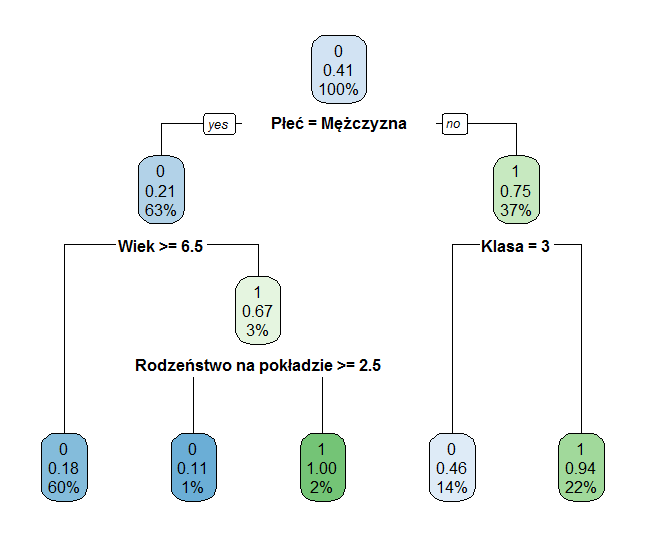
\includegraphics[scale=0.8]{./rys001}

\caption{Wizualizacja drzewa decyzyjnego dla zbioru danych na temat pasażerów statku Titanic. \textit{Źródło:} opracowanie własne}\label{rys001}
\end{figure}

Na przestrzeni lat powstało wiele implementacji algorytmów drzew decyzyjnych \citep[][]{kass1980,loh1997,kim2001}, jednak najczęściej spotykane są trzy wersje: 
\begin{itemize}
\item ID3 (ang.~\textit{Iterative Dichotimiser 3}) – algorytm skonstruowany przez Rossa Quinlana, który stał się prekursonem do algorytmu C4.5. Stosowany tylko do problemów klasyfikacji (zmienna celu jest kategoryczna).
\item C4.5 – poprawiona przez Quinlana wersja algorytmu ID3, pozwalająca na używanie zmiennych ciągłych oraz obecność braków w danych. Obecnie jest również dostępna wersja C5.0, zoptymalizowana pod względem czasochłonności pracy algorytmu.
\item CART (ang.~\textit{Classification And Regression Trees}) – algorytm charakteryzuje się konstrukcją drzew binarnych – każdy wewnętrzy węzeł ma dokładnie dwie wychodzące gałęzie). Tak samo jak C4.5 nadaje się do problemów klasyfikacji i regresji oraz jest w stanie poradzić sobie z brakami danych.
\end{itemize}

Wszystkie powyższe algorytmy dokonują budowy drzewa w sposób rekurencyjny od korzenia do liścia, metodą „dziel i zwyciężaj” (ang.~\textit{divide-and-conquer approach}).  Możemy też zauważyć, że drzewa decyzyjne mogą być klasyfikacyjne bądź regresyjne (odpowiednio dla zmiennej objaśnianej kategorycznej bądź ciągłej). W pierwszym przypadku wartość otrzymana w liściach dla zbioru treningowego jest modą z obserwacji przypadających do danego regionu decyzyjnego. W przypadku drzew regresyjnych otrzymana wartość jest średnią.

Proces budowy drzew klasyfikacyjnych składa się z dwóch etapów: indukcji (ang.~\textit{induction}) oraz przycinania (ang.~\textit{pruning}). Indukcja drzewa jest zadaniem, w którym po wczytaniu danych rekursywnie podejmowana jest decyzja o wybraniu zmiennych najlepiej nadających się do dokonania podziału oraz przeprowadzana jest dzielenie zbioru, do momentu, kiedy wszystkie obserwacje ze zbioru treningowego nie zostaną zaklasyfikowane. Podczas budowy drzewa celem jest taki podział danych względem zmiennych objaśniających, aby wynikające liście zawierały jak najbardziej homogeniczne instancje. Jednocześnie zależy nam na jak najmniejszej ilości podziałów niezbędnych do przypisania wszystkich rekordów (w celu przejrzystości oraz zmniejszenia ryzyka przeuczenia modelu). Widać więc, że decyzja o rozdzieleniu zbioru w dużym stopniu wpływa na skuteczność predykcji drzewa. Kryterium tej decyzji jest różne dla drzew klasyfikacyjnych i regresyjnych, ale także dla różnych algorytmów. Do najważniejszych zaliczamy:
\begin{itemize}
\item Indeks Giniego – działa dla kategorycznych zmiennych celu, tylko w przypadku binarnego podziału zbioru (używany jest w algorytmie CART). Im wyższa wartość współczynnika tym większa homogeniczność.
\item Przyrost informacji (ang.~\textit{Information Gain}) – używa entropii (inaczej teoria informacji) do pomiaru stopnia dezorganizacji danych w liściach. W przypadku kompletnej homogeniczności (liść zawiera tylko obserwacje przynależące do jednej klasy) entropia jest równa 0, natomiast kiedy obserwacji z każdej klasy jest taka sama ilość, wtedy miara przyjmuje wartość 1. Należy pamiętać, że użycie tej miary może prowadzić do przeuczenia modelu. Dzieje się tak ze względu na obciążenie względem zmiennych, które przyjmują wiele wartości (np. zmienne kategoryczne o wielu poziomach). W przypadku występowania takich zmiennych, algorytm ma tendencje do wybierania ich na podziału zbioru, a to prowadzić może do budowy drzewa, które będzie zbyt dopasowane do danych treningowych. Information Gain wykorzystywany jest w algorytmie ID3.
\item Współczynnik przytostu (ang.~\textit{Gain ratio}) – miara stosowana między innymi w algorytmie C4.5, stanowiąca modyfikacje Information Gain. Zmniejsza obciążenie powstałe w wyniku jego użycia poprzez wzięcie pod uwagę informacji wewnętrznej (ang.~intrinsic information) do podziału drzewa. Informacja wewnętrzna zawiera informacje o rozmiarze i liczbie gałęzi.
\end{itemize}

Pseudokod budowy drzewa za pomocą algortmu ID3 został przedstawiony poniżej:

\begin{algorithm}
\renewcommand\thealgorithm{}
\caption{ID3}
\begin{algorithmic} \label{schemat1}
\REPEAT
\STATE $maxGain \leftarrow 0$ \COMMENT{$maxGain$ - maksymalny przyrost informacji} 
\STATE $splitX \leftarrow Null$ \COMMENT{$splitX$ - zmienna po której dokonany ma zostać podział zbioru}
\STATE $entropia \leftarrow Entropia($Predyktory$)$
\FORALL{Predyktory $x$}
\STATE $gain \leftarrow InformationGain(x, entropia)$
\IF{$gain > maxGain$}
\STATE $maxGain \leftarrow gain$
\STATE $splitX \leftarrow x$
\ENDIF
\ENDFOR
\STATE Podział zbioru według zminnej $splitX$
\UNTIL{Wszystkie możliwe podziały zbioru nie zostaną przetworzone}
\end{algorithmic}
\addtocounter{algorithm}{-1}
\end{algorithm}

Może się okazać, że skonstruowane drzewo ma zbyt skomplikowaną strukturę, a z tego względu jest trudne w interpretacji \citep{mingers1989}. Przycinanie drzewa jest procesem, mającym na celu usunięcie niepotrzebnej struktury tak, aby poprawić przejrzystość, ale przede wszystkim żeby zapobiec przeuczeniu. Tak jak w przypadku wyboru kryterium podziału drzewa, również metoda przycinania jest zależna od wybranego algorytmu. Przykładowo, algorytm C4.5 dokonuje przycięcia po konstrukcji drzewa (ang.~\textit{post-prunning}), podczas gdy istnieją techniki pozwalające na dokonanie tego w trakcie procesu budowy (ang.~\textit{pre-prunning}). Pre-prunning nie przeprowadza dosłownie przycinania (nigdy nie przycinają istniejących już gałęzi). Zamiast tego z wyprzedzaniem ucinają poprzez zahamowanie wzrostu gałęzi, kiedy po dodatkowej strukturze nie jest oczekiwane, że zwiększy moc predykcyjną. Więcej o technikach przycinania można przeczytać w pracy \citet{frank2000}. Warto jednak dodatkowo wspomnieć o ograniczeniach, które możemy nałożyć na algorytm przed konstrukcją drzewa. Do grupy parametrów mających wpływ na ryzyko przeuczenia modelu możemy zaliczyć minimalną liczbę obserwacji potrzebną do podziału węzła, minimalną liczbę obserwacji wymaganą w liściach oraz maksymalną głębokość drzewa. Ponadto istnieje możliwość zdefiniowania maksymalnej liczby liści oraz maksymalnej liczby zmiennych, branych pod uwagę do podziału drzewa na danym kroku (zmienne wybierane są w sposób losowy). 

Największa zaleta drzew decyzyjnych leży w ich interpretowalności. Wynik działania algorytmu jest bardzo prosty do zrozumienia, nawet dla osób, które nie mają doświadczenia w analizie danych. Nie jest wymagana żadna statystyczna wiedza, by móc je czytać i interpretować. Z tego wniosku wynika również, iż technika ta jest użyteczna w eksploracji danych. W krótkim czasie jesteśmy w stanie zidentyfikować najbardziej istotne zmienne oraz relacje między nimi. To z kolei przekłada się na możliwość konstrukcji takich zmiennych, które będą charakteryzowały się większą mocą predykcyjną. Niewrażliwość algorytmu na braki danych i obserwacje odstające pozwalają użytkownikowi zaoszczędzić czas na czyszczeniu danych w porównaniu z innymi algorytmami predykcyjnymi. Drzewa decyzyjne są metodą nieparametryczną, co oznacza, że algorytm nie czyni żadnych założeń \textit{apriori} odnośnie struktury klasyfikatora czy rozkładu zmiennej celu. Jeżeli chodzi o wady, zdecydowanie największa leży w możliwości zbytniego dopasowania się do danych treningowych (ang.~\textit{over-fitting}).  W takim przypadku otrzymujemy klasyfikator, który ma wysoką skuteczność na zbiorze uczącym (ze względu na zbyt dokładne zapamiętanie struktury danych), jednak jego użyteczność na zbiorze testowym drastycznie spada. Z tego względu ważne jest przycinanie drzew, jak i nakładanie pewnych ograniczeń w momencie ich konstrukcji. Ponadto, modelując zmienną ciągłą tracimy część informacji w wyniku kategoryzacji zmiennych.


\subsection{Lasy losowe}

Historia algorytmu lasów lowowych sięga 1995 roku, kiedy \citet{ho1995} dowiódł, że problem słabej generalizacji drzew decyzyjnych może być przezwyciężony poprzez zastosowanie wielu drzew. Jego metoda polegała na budowaniu drzew w losowych podprzestrzeniach zmiennych. Ho wnioskował, że drzewa w różnych podprzestrzeniach generalizują wiedzę w sposób komplementarny, a łącząc wyniki ich klasyfikacji możemy zwiększać skuteczność monotonicznie. Ten ostatni wniosek jest sprzeczny z przekonaniem, że zwiększenie złożoności klasyfikatora w celu poprawy jego zdolności predykcyjnej może następować tylko do pewnego momentu, kiedy nie dojdzie do przeuczenia. Dowód przeciwko temu stwierdzeniu, w przypadku metody lasów, można znaleźć w pracach dotyczących teorii dyskryminacji stochastycznej \citep[][]{kleinberg1996, kleinberg2000}. Algorytm w postaci, która jest obecnie używana w pakietach statystycznych został zaproponowany przez Leo Breimana w 2001 roku \citep{breiman2001}.

W przypadku klasyfikacji algorytm lasów losowych dokonuje konstrukcji wielu drzew decyzyjnych. Aby dokonać klasyfikacji nowej obserwacji używamy, jako wsadu zmiennych objaśniających do wszystkich drzew w lesie i zapisujemy wyniki. Następnie dokonujemy głosowania, a klasa która najczęściej pojawia się w drzewach zostaje wybrana. Przykładowa wizualizacji 6 drzew decyzyjnych zbudowanych zgodnie z algorytmem lasów losowych przestawia rysunek~\ref{rys001a}.

\begin{figure}
\centering
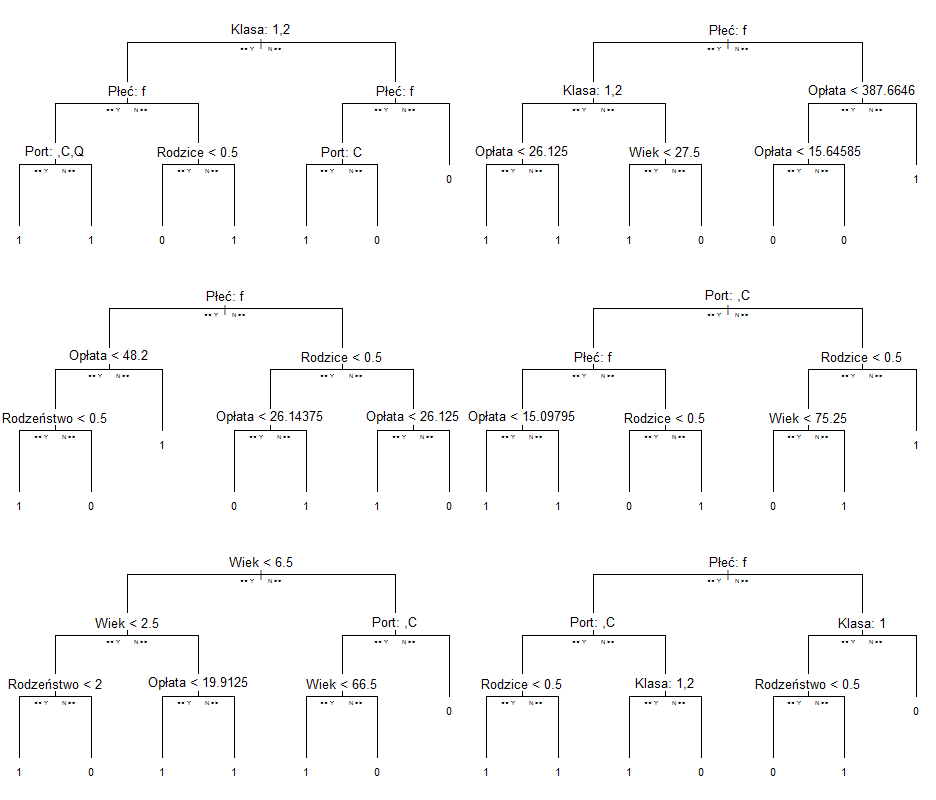
\includegraphics[scale=0.7]{./rys001a}
\caption{Wizualizacja 6 drzew decyzyjnych z lasu losowego dla zbioru danych na temat pasażerów statku Titanic. \textit{Źródło:} opracowanie własne}\label{rys001a}
\end{figure}


Budowa każdego drzewa odbywa się według następującego schematu:
\begin{enumerate}
\item Część oryginalnego zbioru danych zostaje wylosowana ze zwracaniem. Próbka ta będzie służyć za zbiór treningowy.
\item Przyjmijmy że w zbiorze występuje M zmiennych objaśniających. Definiowana jest liczba m, mniejsza od M, używana do losowego wyboru zmiennych, z których na każdym kroku jedna używana jest do podziału węzła. Liczba m pozostaje stała podczas całego procesu budowania lasu. Najczęściej wartością domyślną m jest pierwiastek kwadratowy z wszystkich dostępnych zmiennych niezależnych.
\item Drzewo budowane jest bez żadnych restrykcji oraz bez przycinania.
\end{enumerate}

Błąd powstały w wyniku działania lasów losowych zależy od dwóch czynników. Pierwszym z nich jest korelacja między różnymi dwoma drzewami w lesie. Zwiększona korelacja powoduje zwiększenie błędu. Drugim aspektem jest siła (moc predykcyjna) każdego drzewa. Drzewo z niską wartością błędu jest silnym klasyfikatorem, a zatem zwiększając siłę pojedynczych drzew zmniejszymy błąd w całym lesie. Jedyny parametr, który ma wpływ na działanie lasów losowych to liczba m (liczba zmiennych losowanych). Zmniejszając ją, zmniejszamy korelacje i siłę drzew, a zwiększając otrzymujemy przeciwny rezultat. Dlatego ważne jest znalezienie optymalnego jej przedziału.

Godny odnotowania jest fakt braku konieczności użycia osobnego zbioru testowego (albo przeprowadzenia kroswalidacji), w celu oszacowania błędu. Dzieje się tak, ponieważ każde drzewo konstruowane jest z użyciem innej bootstrapowej próby. Około $1/3$ obserwacji jest pozostawiona poza nią. Po zbudowaniu drzew, dla każdej obserwacji z oryginalnego zbioru wybieramy te próby bootstrapowe, w których te obserwacje nie występują. Następnie używamy ich do klasyfikacji, używając drzew zbudowanych na zbiorach tych prób. Porównujemy otrzymane prognozy z prawdziwymi klasami, a błąd jaki w ten sposób otrzymujemy jest błędem OOB (ang.~\textit{out-of-bag}). Błąd ten jest ważny, ponieważ zostało udowodnione empirycznie \citep{breiman1996}, iż jest tak samo dokładny jak użycie zbioru testowego o takiej samej wielkości, co zbiór uczący. Dlatego używając błędu OOB pozbywamy się potrzeby posiadania osobnego zbioru testowego, co przy danych niewielkich rozmiarów może mieć duże znaczenie.

Ponadto „efektem ubocznym” działania algorytmu lasów losowych jest stworzenie rankingu zmiennych. Dzięki temu, mimo że nie mamy możliwości wyświetlenia całego procesu decyzyjnego (tak jak w drzewie decyzyjnym), możemy przestudiować, które zmienne sprawdzają się najlepiej w całym algorytmie. W celu wyliczenia istotności dla konkretnej zmiennej przeprowadzony jest następujący schemat:
\begin{enumerate}
\item Dla każdego drzewa dokonywana jest klasyfikacja używając obserwacji OOB i porównanie z prawdziwymi wartościami klas. 
\item Następuje permutacja wybranej zmiennej, po której dokonywana jest klasyfikacja (taka sama jak w punkcie 1. i porównanie z prawdziwymi wartościami klas.
\item Od liczby poprawnie zaklasyfikowanych przypadków dla permutowanego zbioru odejmowana jest liczba poprawnie zaklasyfikowanych przypadków dla niezmienionych danych.
\item Schemat ten powtarzany jest dla wszystkich drzew, a na końcu obliczana jest średnia różnica z punktu 3.
\end{enumerate}

W przypadku kiedy wartości policzonej istotności są niezależne między drzewami, możemy policzyć błąd standardowy. Błąd ten używany jest do wyliczenia zeskalowanej istotności danej zmiennej (ang.~\textit{z-score}). Jeśli liczba zmiennych w zbiorze jest duża, las losowy może być uruchomiony używając wszystkich zmiennych, a następnie używając tylko istotnych zmiennych otrzymanych w pierwszym kroku.

Lasy losowe pozwalają na obliczenie bliskości (ang.~\textit{proximity}) pomiędzy parami kolejnych obserwacji. Po skonstruowaniu drzewa, zarówno obserwacje treningowe, jak i obserwacje OOB stanowią jego wsad. W przypadku gdy dwie obserwacje znajdują się w tym samym liściu, w obrębie tego samego drzewa, ich bliskość wzrasta o jeden. Gdy cały las zostaje zbudowany, wartości podobieństw zostają znormalizowane używając liczby drzew. Bliskości używane są do zastępowania braków danych, lokalizacji obserwacji odstających, a także tworzenia wizualizacji danych poprzez redukcję wymiaru.

Częstym problemem pojawiającym się przy klasyfikacji jest niezbilansowanie próby. Niezbilansowanie oznacza w tym przypadku nadreprezentację jednej z klas zmiennej objaśnianej i objawia się najczęściej w sytuacjach, kiedy istnieje potrzeba predykcji zdarzenia występującego relatywnie rzadko (np. bankructwa firm, wykrycia rzadko występującego nowotworu). Starając się zminimalizować całkowity błąd, algorytm lasów losowych (ale także inne algorytmu uczenia maszynowego) utrzyma błąd na bardziej liczebnej klasie na niskim poziomie, podczas gdy na drugiej pozwoli na wysoki stopień błędu. Las losowy pozwala na zbalansowanie błędu poprzez ustawienie różnych wag dla poszczególnych klas. Im wyższa waga dla danej klasy, tym w większym stopniu zostanie on zredukowany. Dobrą radą jest ustawienie wagi jako odwrotnie proporcjonalnej do stosunku liczebności klas. 

Jak widać, zalet lasów losowych można wymienić wiele. Przede wszystkim, w przeciwieństwie do drzew decyzyjnych obarczone są mniejszym ryzykiem przeuczenia. Po drugie są w stanie poradzić sobie z dużą ilością zmiennych oraz obserwacji. Pozwalają na stworzenie rankingu zmiennych, a korzystanie z błędu OOB nie wymusza konieczności trzymania osobnego zbioru testowego. Należy jednak pamiętać o ograniczeniach. Lasy losowe postrzegane są jako algorytm czarnej skrzynki (ang.~\textit{black box}), ponieważ składają się z losowo wygenerowanych drzew decyzyjnych, które nie są podyktowane żadnymi wytycznymi w predykcji. Przykładowo nie jesteśmy w stanie ocenić dokładnie dlaczego model zdecydował o odrzuceniu wniosku kredytowego dla konkretnego klienta. Wiemy tylko tyle, że większość spośród drzew w lesie była takiego zdania. Taka konstrukcja może powodować, że w pewnych dziedzinach (np. zastosowania medyczne) przydatność tego algorytmu będzie kwestionowana, mimo wysokiej skuteczności. Ponadto lasy losowe nie nadają się do ekstrapolacji, to znaczy do predykcji jakiegoś zjawiska w warunkach, których algorytm wcześniej nie doświadczył. Przykładowo, jeśli wiadome by było, że jedna gazeta kosztuje dwa złote, dwie gazety kosztują cztery, a pięć kosztuje dziesięć złotych, lasy losowe nie byłyby w stanie podać poprawnej odpowiedzi dla 20 gazet, jeśli w zbiorze treningowym nie spotkały się z takim przypadkiem. 

\subsection{Algorytm K-najbliższych sąsiadów}

Algorytm K-najbliższych sąsiadów (ang.~\textit{K-Nearest Neighbors}) jest metodą nieparametryczną, służącą do problemów klasyfikacji i regresji. Nieparametryczność oznacza, że nie czyni ona żadnych założeń odnośnie rozkładu danych, co powoduje że staje się użyteczna do badania nieliniowych związków w danych. Jest to metoda wyjątkowa spośród innych narzędzi uczenia maszynowego, ponieważ nie odbywa się w niej faza uczenia na podstawie zbioru w celu generalizacji wiedzy w niej zawartej. Zamiast tego, algorytm zobligowany jest trzymać cały zbiór treningowy, którego używa w procesie predykcji na zbiorze testowym. Jest to podejście przeciwne do stosowanych w innych algorytmach, np. SVM, gdzie usuwane są nieprzydatne wektory nośne.

Metoda najbliższych sąsiadów zakłada, że dane znajdują się w przestrzeni zmiennych objaśniających (ang.~\textit{feature space}), czyli są w przestrzeni metrycznej. Dane mogą być skalarami bądź też wielowymiarowymi wektorami. To założenie powoduje, że jesteśmy w stanie policzyć wartość metryki (najczęściej odległość euklidesową, ale także wykorzystuje się odległość Mahalanobisa). Ponadto, zakłada się że dane, oprócz wektorów je opisujących posiadają także zmienną celu, która może mieć charakter dyskretny i składać się z dwóch lub więcej klas, a także być ciągła. Jedynym parametrem, którym możemy sterować jest liczba $K$, określająca ile sąsiadów wpływa na klasyfikacje. 

Predykcje dla nowych danych dokonywane są w trzech krokach:
\begin{enumerate}
\item Obliczenie odległości (za pomocą wybranej miary) pomiędzy nową obserwacją a wszystkimi punktami ze zbioru treningowego
\item Wybranie $K$ najbliższych sąsiadów, dla których odległość jest najmniejsza
\item W przypadku klasyfikacji przeprowadzane jest głosowanie w celu wyboru klasy, natomiast dla regresji wynik jest średnią z wartości zmiennej objaśnianej dla sąsiadów
\end{enumerate}

Wybór odpowiedniej miary odległości powinien być dokonany na podstawie właściwości badanych danych. Jeśli zmienne objaśniające są podobnego typu (np. są wyrażone w tych samych jednostkach, jak długość czy szerokość obiektu) rozsądne może być wybranie odległości euklidesowej. Kiedy zmienne nie mają zbliżonego charakteru (np. płeć, wiek, wzrost, waga), wtedy użycie metryki miejskiej może być odpowiednie. Poza wyborem miary odległości, kluczowy jest wybór liczby sąsiadów, która jest brana do prognozy zmiennej celu. W przypadku zbioru treningowego, najmniejszy błąd będziemy otrzymywać zawsze dla $K = 1$ (błąd będzie równy 0). Bierze się to z faktu, że w tym przypadku najbliższy punkt do każdej obserwacji ze zbioru uczącego to w istocie ten sam punkt. Jeśli taki sam wynik otrzymywalibyśmy na zbiorze walidacyjnym, wtedy zawsze naszym wyborem byłoby$K = 1$. Jest to jednak przykład, dla którego algorytm zbyt bardzo dopasowuje się do danych, co skutkuje wysokim błędem na zbiorze walidacyjnym (również na zbiorze testowym). Wysokie wartości $K$ skutkują również wysokimi błędami, jako że do predykcji biorą pod uwagę także obserwacje niepodobne względem badanego punktu. Dlatego też celem jest wybór pośredniego $K$, które z jednej strony nie bierze pod uwagę szumu występującego w danych, a z drugiej nie czyni zbyt ogólnej generalizacji. Rozwiązaniem jest testowanie różnych kombinacji parametru, bądź stosowanie technik walidacji krzyżowej.

Należy pamiętać, że algorytm KNN sprawdza się dobrze w sytuacjach gdy mamy mało zmiennych niezależnych \citep{indyk1998}. Każda zmienna może być postrzegana jako wymiar w przestrzeni $X$-wymiarowej (gdzie $X$ oznacza liczbę dostępnych zmiennych). Okazuje się, że wraz ze wzrostem wymiarów (zmiennych objaśniających), eksponencjalnie wzrasta liczebność próby niezbędnej do funkcjonowania algorytmu. To powoduje, że w wysokich wymiarach punkty, które są podobne mogą charakteryzować się dużą odległością. Zjawisko to znane jest jako przekleństwo wymiaru (więcej na ten temat pisze \citet{hastie2009}).

Mimo niewątpliwych zalet tego algorytmu, trzeba wziąć pod uwagę konieczność obróbki danych, w celu otrzymania lepszych rezultatów. Do tych działań możemy zaliczyć przeskalowanie danych. Zależy nam bowiem na tym, aby zmienne były na tej samej skali. W tym celu dobrym pomysłem jest normalizacja danych, tak aby znajdowały się w przedziale $<0,1>$ , bądź też standaryzacja, tak aby zmienne charakteryzowały się rozkładem normalnym. Ponadto niezbędna jest interwencja w kierunku braku danych (tak aby kalkulacja odległości między kolejnymi obserwacjami była możliwa), a także selekcja zmiennych w celu zmniejszenia wielowymiarowości.

\subsection{Regresja logistyczna}

Regresja logistyczna jest modelem zaproponowanym przez Davida Coxa \citep{cox1958}, używanym do szacowania prawdopodobieństwa zmiennej binarnej na podstawie jednej lub więcej zmiennych objaśniających. Swoją nazwę zawdzięcza funkcji logistycznej (rysunek~\ref{rys002}), która może przyjąć jako argument dowolną wartość rzeczywistą i mapować ją na wartość z przedziału $(0,1)$. 

\begin{figure}
\centering
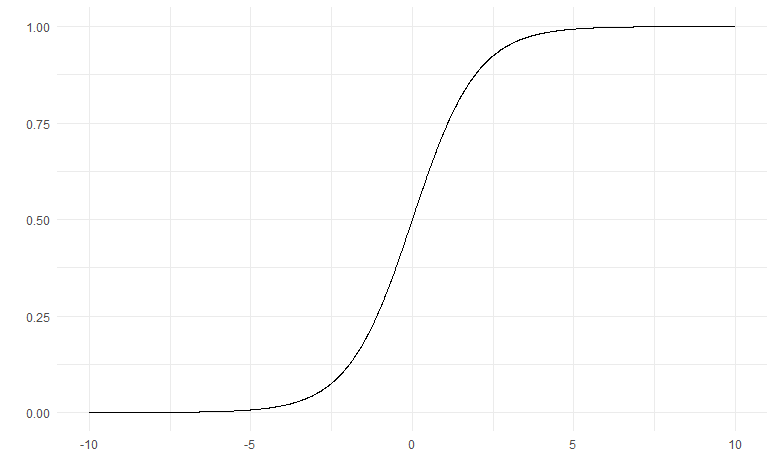
\includegraphics[scale=0.7]{./rys002}
\caption{Wykres funkcji logistycznej. \textit{Źródło:} opracowanie własne}\label{rys002}
\end{figure}

Weźmy jako przykład modelowanie prawdopodobieństwa spłaty kredytu hipotecznego za pomocą jednej zmiennej objaśniającej. Używając do tego celu regresji liniowej prawdopodobieństwa byłyby reprezentowane za pomocą wzoru~\ref{wzor1}:

\begin{equation} \label{wzor1}
p(x) = \beta_0 + \beta_1x
\end{equation}

Tym sposobem jednak otrzymalibyśmy prawdopodobieństwa spoza przedziału $(0,1)$, co nie byłoby zgodne z aksjomatyczną definicją prawdopodobieństwa. Dlatego też konieczne jest użycie funkcji logistycznej (bądź innej zwracającej wynik pomiędzy zero a jeden) do modelowania tego zjawiska. W takim przypadku model byłby następującej postaci:

\begin{equation} \label{wzor2}
p(x) = \frac {e^{\beta_0 + \beta_1x}} {1 + e^{\beta_0 + \beta_1x}}
\end{equation}

Współczynniki tego modelu (\ref{wzor2}) szacowane są za pomocą metody największej wiarygodności (ang.~\textit{maximum-likelihood estimation}). Intuicja stojąca za tą metodą to poszukiwanie wartości parametrów, które minimalizują błąd przewidywanych prawdopodobieństw w stosunku do wartości prawdopodobieństw ze zbioru treningowego. W praktyce używany jest efektywny numerycznie algorytm optymalizacyjny (np. metoda quasi-Newtona).

Przekształcając wzór~\ref{wzor2} otrzymujemy:

\begin{equation} \label{wzor3}
\frac{p(x)}{1 - p(x)} = e^{\beta_0 + \beta_1x}
\end{equation}

Lewa strona równania~\ref{wzor3} przedstawia szanse (ang.~\textit{odds}) zajścia modelowanego zjawiska i przyjmuje wartości pomiędzy zerem a nieskończonością. Wartości bliskie zera oznaczają niskie prawdopodobieństwa wystąpienia zdarzenia, natomiast bliskie nieskończoności wysokie. Szanse używane są np. w zakładach bukmacherskich, zamiast prawdopodobieństw, ponieważ lepiej obrazują stosunek pomiędzy prawdopodobieństwem zwycięstwa a przegranej. Stosując logarytm po obu stronach równania we wzorze 3 otrzymujemy:

\begin{equation} \label{wzor4}
\ln \frac{p(x)}{1 - p(x)} = \beta_0 + \beta_1x
\end{equation}

Lewa strona równania~\ref{wzor4} nazywana jest logarytmem szans bądź logitem. W modelu regresji liniowej oszacowanie parametru stojącego przy danej zmiennej objaśniającej oznaczało średnią zmianę wartości zmiennej celu związanej z jednostkowym przyrostem zmiennej niezależnej. W przypadku regresji logistycznej wzrost o jednostkę predyktora przekłada się na wzrost logarytmu szans o $\beta_1$, bądź równoważnie na przemnożenie szans przez $e^{\beta_1}$.

Dokonując predykcji dla nowych danych konieczne jest podstawienie wartości zmiennych objaśniających do wzoru~\ref{wzor2}, po estymacji współczynników metodą największej wiarygodności. Jako wynik otrzymujemy wartość prawdopodobieństwa (ang.~\textit{score}) modelowanej kategorii zmiennej objaśnianej. W naszym przypadku byłoby to prawdopodobieństwo spłaty kredytu. Należy zadać sobie pytanie, w jaki sposób transformować otrzymaną wartość na binarną zmienną. Odpowiedzią jest odpowiednie dobranie progu odcięcia. Standardowo przyjmuje się próg odcięcia równy 0.5 (1 dla wartości prawdopodobieństwa większej bądź równej 0.5; 0 w przeciwnym wypadku). W pewnych sytuacjach jednak bardziej rozsądnym będzie użycie innego progu. Taka sytuacja występuje np. w naszym przykładzie. Dla nowego klienta bank będzie chciał dokonać predykcji tego czy spłaci kredyt hipoteczny czy też nie. Przyznanie wnioskodawcy kredytu obarczone jest ryzykiem niespłacenia go, natomiast odmówienie wiąże się z kosztem utraconych korzyści w momencie kiedy kredytobiorca dopełniłby swojej umowy. Te dwa czynniki powinny być brane pod uwagę przy ustalaniu wielkości progu odcięcia – zbyt niska jego wartość przekładałaby się niechybnie na większą stratę z tytułu niespłaconych kredytów, a zbyt wysoki z utratą możliwych do osiągnięcia zysków. W praktyce wartość progu odcięcia ustalana jest za pomocą metod walidacji krzyżowej.

Należy pamiętać o założeniach czynionych przez regresję logistyczną. Dosyć oczywistą i omawianą już wcześniej jest konieczność modelowania zmiennej objaśnianej, która jest zero-jedynkowa. Ponadto regresja logistyczna jest liniowym algorytmem (z nieliniowym przekształceniem na zmienną zależną), który zakłada liniowy związek pomiędzy zmiennymi objaśniającymi a zmienną celu. Dlatego jeśli możliwa jest transformacja predyktorów, która lepiej uwidoczni tą zależność to należy jej użyć, jako że może przekładać się na bardziej dokładny model. Zmienne silnie ze sobą skorelowane mogą prowadzić do przeuczenia modelu bądź niezdolności metody największej wiarygodności do zbieżności (co skutkuje w braku oszacowań parametrów), dlatego należy pozbyć się ich przed modelowaniem. Dodatkowo wskazane jest wykrycie i wyeliminowanie obserwacji odstających. 

\subsection{Liniowa oraz kwadratowa analiza dyskryminacyjna}

Jak już zostało wcześniej wspomniane, regresja logistyczna pomimo niewątpliwych zalet posiada także ograniczenia. Przede wszystkim nie nadaje się do modelowanie zmiennych posiadających więcej niż dwie kategorie. Ważna jest też stabilność otrzymanych parametrów. Okazuje się, że gdy klasy zmiennej celu są dobrze od siebie odseparowane, parametry otrzymane za pomocą regresji logistycznej wykazują się dużą niestabilnością. To samo wynika w przypadku posiadania niewielkiej liczby obserwacji oraz kiedy predyktory charakteryzują się rozkładem normalnym dla każdej klasy. Rozwiązaniem tych problemów jest zastosowanie liniowej analizy dyskryminacyjnej (ang.~\textit{linear discriminant analysis}). 

Algorytm ten, bazujący na pracy Ronalda Fishera z 1936 roku \citep{fisher1936}, korzysta ze statystycznych własności danych policzonych dla każdej klasy. W przypadku gdy mamy do czynienia z jedną zmienną objaśniającą jest to średnia i wariancja zmiennej dla każdej klasy. Natomiast gdy istnieje więcej zmiennych egzogenicznych, wyliczane są kolejne średnie oraz macierz kowariancji. 

Jeśli chodzi o założenia, liniowa analiza dyskryminacyjna zakłada, że rozkład każdej zmiennej jest rozkładem normalnym oraz że każda zmienna ma taką samą wielkość wariancji. Z tymi założeniami, oszacowanie średniej i wariancji wszystkich zmiennych dla każdej kategorii zmiennej objaśnianej dokonuje się w sposób standardowy. 

Liniowa analiza dyskryminacyjna dokonuje predykcji dla nowej obserwacji poprzez oszacowanie prawdopodobieństwa przynależności do kolejnych klas. Kategoria która otrzymuje największe prawdopodobieństwo jest kategorią wynikową z modelu. Do oszacowania wielkości prawdopodobieństwa model korzysta z twierdzenia Bayesa:

\begin{equation} \label{wzor5}
p(Y = k | X = x) = \frac{p(k)p(X = x | Y = k)}{\sum_{l = 1}^{K} p(l)p(X = x | Y = l)} 
\end{equation}

gdzie:
\begin{itemize}
\item $p(Y=k | X=x)$ – prawdopodobieństwo przynależności do klasy k obserwacji x.
\item$ p(k)$ – prawdopodobieństwo \textit{a priori} (prawdopodobieństwo bazowe przynależności kategorii k w zbiorze treningowym – w przypadku gdy liczba kategorii jest równa 2, a dane są zbilansowane, prawdopodobieństwo to będzie równe 0.5)
\item $p(X=x | Y=k)$ – wyestymowane prawdopodobieństwo przynależności obserwacji do klasy $k$. Innymi słowy jest to funkcja gęstości zmiennej/zmiennych objaśniających $X$ dla obserwacji, która pochodzi z klasy $k$. Funkcja ta przyjmuje wysokie wartości kiedy istnieje duże prawdopodobieństwo, że obserwacja w klasie $k$ ma wartość zmiennej/zmiennych objaśniających ($X$) w przybliżeniu równą wartości obserwacji ($x$).
\end{itemize}

Oszacowane prawdopodobieństwo przynależności obserwacji do danej klasy można zapisać za pomocą funkcji gęstości rozkładu normalnego. Podstawiając funkcję do wzoru~\ref{wzor5} oraz wyciągając logarytm otrzymujemy:

\begin{equation} \label{wzor6}
\hat{\delta_k}(x) = x \frac{\hat{\mu_k}}{\hat{\sigma^2}} - \frac{\hat{\mu_k^2}}{2\hat{\sigma_k^2}} + \log(\hat{p(k)})
\end{equation}

gdzie: 
\begin{itemize}
\item $\hat{\mu_k}$ - oszacowanie średniej dla każdej kategorii zmiennej objaśniającej
\item $\hat{\sigma^2}$ - oszacowanie wariancji dla każdej kategorii zmiennej objaśniającej
\item $\hat{p(k)}$ - oszacowanie prawdopodobieństwa bazowego
\end{itemize}
 Wzór~\ref{wzor6} określany jest mianem funkcji dyskryminacyjnej. Klasa dla której wartość tej funkcji jest największa wybierana jest jako przewidywana klasyfikacja.

Przygotowując dane do użycia na nich algorytmu liniowej analizy dyskryminacyjnej trzeba brać pod uwagę kilka aspektów. Przede wszystkim należy pamiętać o założeniach tego algorytmu. Z tego względu dobrym pomysłem jest standaryzacja danych, tak aby każda zmienna charakteryzowała się średnią równą zero oraz odchyleniem standardowym równym jeden.  Dobrze jest też pozbyć się obserwacji odstających (żeby nie zaburzały statystyk) oraz dokonać transformacji w przypadku rozkładu zmiennych różnych od normalnego (zastosowanie logarytmu bądź pierwiastka kwadratowego w przypadku rozkładu zbliżonego do wykładniczego oraz transformacji Boxa-Coxa dla rozkładów skośnych).

Warto także wspomnieć o rozszerzeniu algorytmu LDA zwanym kwadratową analizą dyskryminacyjną (ang.~\textit{quadratic discriminant analysis}), która ma podobne założenia, jednak zakłada że każda klasa posiada różną macierz kowariancji. Założenie to okazuje się być racjonalne, kiedy zbiór treningowy jest duży. Ponadto QDA stanowi pewnego rodzaju kompromis pomiędzy  algorytmem K najbliższych sąsiadów a liniową analizą dyskryminacyjną i regresją logistyczną. Pozwala ona na modelowanie większej ilości problemów, jako że zakłada kwadratową decyzję decyzyjną (w LDA granica decyzyjna ma postać liniową), a także sprawdza się lepiej przy mniejszej liczbie dostępnych informacji (w porównaniu do algorytmu KNN) poprzez nakładanie pewnych założeń na postać granicy decyzyjnej. Metoda ta jest jednak bardziej złożona obliczeniowa ze względu na większą liczbę parametrów koniecznych do oszacowania. 

\subsection{Metoda wektorów nośnych}

Teoria stojąca za metodą wektorów nośnych (ang.~\textit{Support Vector Machines}) została po raz pierwszy opisana przez Vladimira Vapnika w 1996 roku \citep{vapnik1996}. Najlepszym sposobem jego wytłumaczenia jest przedstawienie klasyfikatora maksymalizującego margines (ang.~\textit{maximal-margin classifier}). Numeryczne zmienne objaśniające w danych tworzą wielowymiarową przestrzeń. W przypadku dwuwymiarowym hiperpłaszczyzna jest linią, która dzieli przestrzeń zmiennych. W metodzie SVM hiperpłaszczyzna jest dobierana tak, aby w najlepszy sposób odseparowała od siebie obserwacje pochodzące z różnych kategorii zmiennej celu. Za pomocą tej linii (bądź płaszczyzny w przypadki gdy liczba zmiennych jest większa od dwóch) jesteśmy w stanie dokonywać klasyfikacji nowych rekordów. Odległość pomiędzy granicą decyzyjną (hiperpłaszczyzną) a najbliższym punktami klas zmiennej objaśnianej nazywany jest marginesem (rysunek~\ref{rys003}). Optymalną linią według algorytmu SVM jest ta, która separuje od siebie klasy maksymalizując margines. Punkty, leżące najbliżej od hiperpłaszczyzny je separującej są nazywane wektorami nośnymi (ang.~\textit{support vectors}) i tylko one istotne są przy wyborze granicy decyzyjnej.

\begin{figure}
\centering
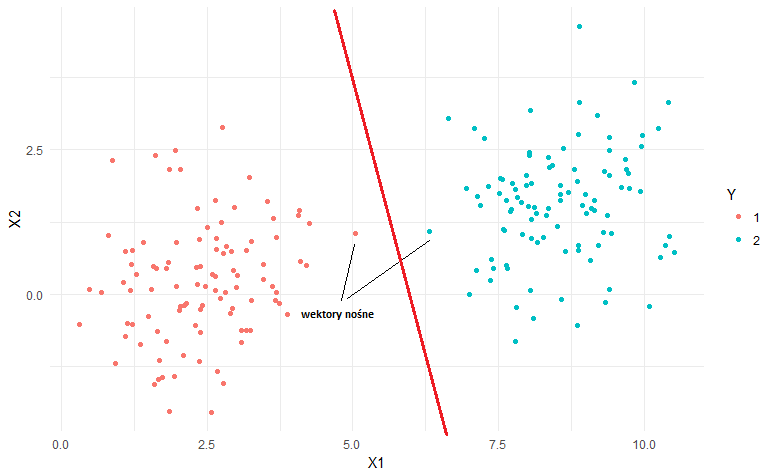
\includegraphics[scale=0.82]{./rys003}
\caption{Graficzna reprezentacja granicy decyzyjnej oraz wektorów nośnych w metodzie SVM. \textit{Źródło:} opracowanie własne}\label{rys003}
\end{figure}

W praktyce jednak dane z różnych klas nadkładają się na siebie tak, że niemożliwe staje się idealne odseparowanie danych za pomocą hiperpłaszczyzny. Dlatego też konieczna jest relaksacja założenia o maksymalizacji marginesu przez klasyfikator. Uproszczenie tego założenia pozwala części punktów ze zbioru treningowego na naruszanie granicy decyzyjnej. Precyzyjniej rzecz ujmując dodatkowe parametry są wprowadzane do modelu, pozwalając marginesowi na ruch w kierunku każdego wymiaru. Parametry te nazywane są czasami dopełniającymi zmiennymi (ang.~\textit{slack variables}). Wprowadzenie ich zwiększa oczywiście złożoność modelu, jako że jest więcej niewiadomych do oszacowania. 

W przypadku gdy dane są liniowo-separowalne, a model nie zawiera zmiennych dopełniających, funkcja dyskryminująca przyjmuje postać taką jak we wzorze~\ref{wzor7}, gdzie $w$ jest wektorem wag, a $b$ jest obciążeniem.

\begin{equation} \label{wzor7}
f(x) = w^Tx + b
\end{equation}

Proces uczenia metody wektorów nośnych może być w takim przypadku sformułowany jako optymalizacja:

\begin{equation} \label{wzor8}
\max_w \frac{2}{||w||} = \min_w ||w||^2
\end{equation}

Jest to problem optymalizacji funkcji kwadratowej z liniowymi warunkami ograniczającymi ($y_i(w^Tx_i + b) \geq 1$), która ma unikalne minimum. Dodając zmienne dopełniające ($\varepsilon_i$) optymalizujemy następujące równanie:

\begin{equation} \label{wzor9}
\min_w ||w||^2 + C\sum_{i}^{N} \varepsilon_i
\end{equation}

przy warunku $y_i(w^Tx_i + b) \geq 1 - \varepsilon_i$

W przypadku, gdy $\varepsilon_i$ jest z przedziału $(0,1>$ punkt ten leży pomiędzy marginesem a poprawną stroną hiperpłaszczyzny. Gdy $\varepsilon_i$ jest większe od jedności wtedy punkt jest niepoprawnie sklasyfikowany. Widzimy także, że pojawia się parametr regularyzacyjny $C$, zwany parametrem kosztu. Jego niskie wartości pozwalają na ignorowanie warunków ograniczających co skutkuje szerokim marginesem. Wysokie wartości powodują powstanie wąskiego marginesu. Gdy wartość parametru $C$ jest równa nieskończoności, wtedy wszystkie warunki ograniczające są narzucone i żaden punkt nie wpada między marginesy. 

Kiedy dane nie są liniowo-separowalne, zostają transformowane do przestrzeni o wyższym wymiarze za pomocą jakieś funkcji, a następnie w tej przestrzeni analogicznie jak poprzednio poszukiwana jest odpowiednia hiperpłaszczyzna. Funkcje, którymi dokonywane jest takie przekształcenie nazywa się funkcjami jądrowymi (ang.~\textit{kernel functions}). Dokładniej rzecz ujmując, funkcje jądrowe są skrótem pozwalającym nam na przeprowadzenie operacji w sposób szybszy niż analogicznych obliczeń w przestrzeni wyższego wymiaru. W najprostszej postaci kernel zdefiniowany jest jako iloczyn skalarny dwóch funkcji $K(x, y) = <f(x), f(y)>$, gdzie $x$, $y$ są obserwacjami z $n$-wymiarowej przestrzeni, a $f$ jest funkcją mapującą przestrzeń $n$-wymiarową na $m$-wymiarową ($m$ jest zazwyczaj dużo większe niż $n$). W normalnej sytuacji policzenie iloczynu skalarnego $<f(x), f(y)>$ wymaga policzenia najpierw $f(x)$ oraz $f(y)$ a następnie iloczynu skalarnego. Operacje te jednak mogą być bardzo kosztowne obliczeniowo, jako że przeprowadzane są w $m$-wymiarowej przestrzeni, po czym i tak w wyniku działania iloczynu skalarnego wracamy do przestrzeni 1-wymiarowej. Obejściem tego problemu są funkcje jądrowe. Dzięki nim łatwo jesteśmy w stanie przejść do przestrzeni o wyższym wymiarze nawet, kiedy zbiór danych składa się z wielu zmiennych objaśniających. Operacja ta znana jest także pod nazwą triku kernelowego (ang.~\textit{kernel trick}). Funkcje jądrowe mogą przyjmować różną postać, np. liniową, wielomianową, sigmoidalną czy radialną, a wybór odpowiedniej powinien zależeć od wiedzy eksperckiej na temat funkcji, która w najlepszy sposób dokonałaby transformacji danych wejściowe na takie, której klasy w łatwy sposób można by odseparować za pomocą hiperpłaszczyzny. Przykładowe przekształcenie sztucznie wygenerowanych danych za pomocą kernelu zostało przedstawione na rysunkach~\ref{rys004a} oraz \ref{rys004b}.

\begin{figure}
\centering
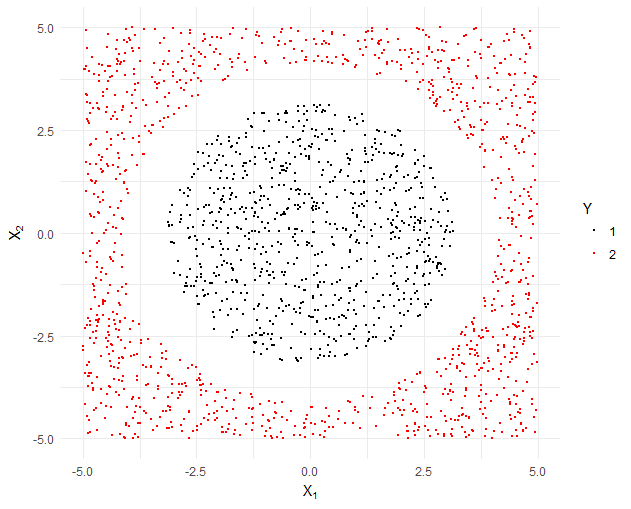
\includegraphics[scale=0.82]{./rys004a}
\caption {Wizualizacja nieliniowo separowalnego zbioru danych, gdzie $X_1$ oraz $X_2$ są zmiennymi objaśniającymi, natomiast zmienna celu $Y$ została zaznaczona kolorem. \textit{Źródło:} opracowanie własne}\label{rys004a}
\end{figure}

\begin{figure}
\centering
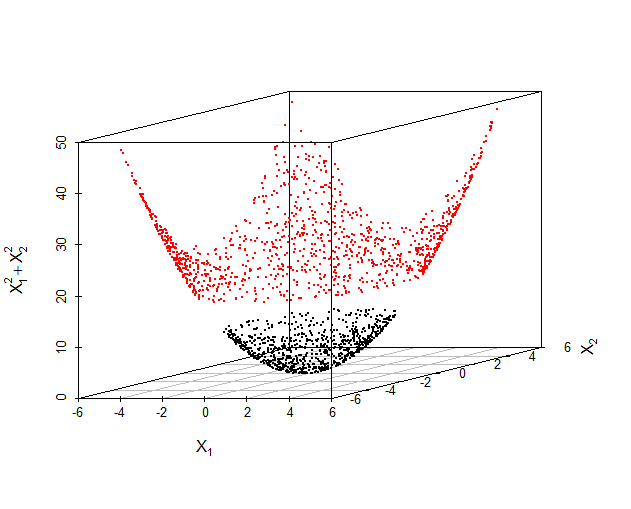
\includegraphics[scale=0.82]{./rys004b}
\caption{Wizualizacja nieliniowo separowalnego zbioru danych przeniesionego do wyższego wymiaru za pomocą funkcji jądrowej. \textit{Źródło:} opracowanie własne}\label{rys004b}
\end{figure}



\subsection{XGBoost}

Algorytm XGBoost (ang.~\textit{Extreme Gradient Boosting}) zbudowany został na bazie pomysłu gradientowego wzmacniania, zaproponowanego w 2001 roku przez Jerome Friedmana \citep{friedman2001}. Podobnie jak algorytm lasów losowych, XGBoost buduje wiele słabych pod względem mocy predykcyjnej drzew decyzyjnych, a następnie używa ich do predykcji. Inny jest natomiast proces łączenia pojedynczych drzew. Intuicyjnie, algorytm ten buduje zespół drzew decyzyjnych, które są dopasowywane sekwencyjnie, w taki sposób, że każde nowe drzewo stara się zmniejszyć błąd poprzedniej wersji modelu.

Idea gradientowego wzmacniania (ang.~\textit{gradient boosting}) opiera się na trzech aspektach:
\begin{enumerate}
\item Funkcja straty – zależy od rozwiązywanego problemu (np. dla regresji może to być błąd średniokwadratowy, a dla klasyfikacji logarytmiczna funkcja straty). Funkcja może być zdefiniowana ręcznie, jednak musi spełniać warunek różniczkowalności.
\item Słaby uczeń (ang.~\textit{weak learner}) – drzewa decyzyjne są używane jako słabi uczniowie. Konstruowane są w sposób chciwy (wybór lokalnie optymalnej decyzji na każdym kroku), tzn. poprzez dobór miejsca podziału drzewa na podstawie funkcji mierzącej homogeniczność węzłów (np. indeks Giniego) bądź minimalizującej stratę. Ponadto nakładane są warunki ograniczające na pojedyncze drzewa, takie jak maksymalna głębokość drzewa, maksymalna liczba węzłów czy liści.
\item Model addytywny – drzewa dodawane są pojedynczo, tak że pozostałe zbudowane wcześniej nie zostają zmienione. Metoda gradientu prostego (ang.~\textit{gradient descent}) jest używana do minimalizacji funkcji straty w trakcie dodawania nowych drzew. Szczegółowiej, po przeliczeniu funkcji straty, algorytm w celu przeprowadzenia metody gradientu prostego musi dodać drzewo, które zmniejsza stratę, czyli podąża za gradientem. Dokonywane jest to poprzez zmianę parametrów drzewa. Wynik nowego drzewa jest następnie dodawany do istniejącej sekwencji modeli. Kryterium stopu algorytmu jest zdefiniowana wcześniej maksymalna liczba drzew, bądź osiągnięcie momentu, w którym nie następuje znacząca poprawa modelu w wyniku dodawania kolejnych drzew.
\end{enumerate}

Oprócz tego ważną częścią jest regularyzacja parametrów, w celu uniknięcia przeuczenia modelu. Pierwszą metoda została już wspomniana wyżej i polega na nakładaniu warunków ograniczających na dodawane drzewa decyzyjne. Druga opiera się na ważeniu udziału każdego drzewa, w celu spowolnienia uczenia modelu (ang.~\textit{shrinkage}; \textit{learning rate}). Tempo uczenia (oznaczane najczęściej w literaturze jako $v$) przyjmuje wartości między zerem a jednością. Im mniejsza wartość, tym więcej iteracji potrzebuje algorytm, a co za tym idzie większa też jest złożoność obliczeniowa. Empirycznie jednak zostało udowodnione, że model w przypadku mniejszych wartości parametru $v$ jest w stanie osiągnąć lepszą generalizację wiedzy \citep{hastie2009}. Ponadto w celu uniknięcia przeuczenia modelu pomocne jest ustalenie frakcji danych treningowych $f$, które używane są do dopasowania drzew w kolejnych krokach. Gdy $f = 1$, algorytm działa bez zmian i cały zbiór danych jest używany. W przypadku mniejszych wartości, tylko próbka danych (wybrana za pomocą losowania bez zwracania) bierze udział w budowie drzew. Friedman w swoim artykule \citep{friedman1999} pokazał że wartości parametru $f$ z przedziału $<0.5, 0.8>$ prowadzą do dobrych rezultatów pod względem skuteczności modelu. Ponadto w przypadku zastosowania tego mechanizmu algorytm działa szybciej, jako że używa mniej danych na każdym kroku do dopasowania drzew oraz liczony jest błąd OOB (patrz podrozdział drewa decyzyjne), dzięki któremu nie ma potrzeby wyodrębniania osobnego zbioru walidacyjnego. Ostatnim sposobem na walkę z przeuczeniem jest nałożenie dodatkowych ograniczeń na parametryzowane drzewa (poza warunkami ograniczającymi związanymi z ich strukturą). Drzewa używane w procesie uczenia są drzewami regresyjnymi, co oznacza że w liściach znajdują się wartości numeryczne. Wartości te, zwane także wagami, mogą podlegać regularyzacji (regularyzacja L1, L2) powodując, że gałęzie, które nie przyczyniają się do znacznego zredukowania straty zostaną przycięte.

Należy zwrócić uwagę, że algorytm XGBoost różni się od standardowej idei gradientowego wzmacniania przede wszystkim strukturą modelu bardziej nastawioną na uniknięcie zjawiska przeuczenia (\url{goo.gl/TmTv1W}). Ponadto swoją nazwę zawdzięcza zorientowaniu na maksymalne wykorzystanie zasobów obliczeniowych, co znacząco przyspiesza pracę algorytmu. 


\chapter{Klasyfikacja kombinowana}

Klasyfikacja kombinowana jest techniką łączenia wielu modeli, głównie w celu poprawy zdolności predykcyjnych w stosunku do stosowania pojedynczych algorytmów. Poza tym zadaniem, łączenie klasyfikatorów pozwala odpowiedzieć na pytanie dotyczące wyboru odpowiedniego algorytmu do danego problemu. Jak zostało pokazane wcześniej, liczba dostępnych modeli jest duża, a każdy z nich może być używany z różnymi wartościami hiperparametrów. Wybór na podstawie jak najmniejszego błędu popełnionego na zbiorze treningowym, nawet używając narzędzi walidacji krzyżowej może być mylący w przypadku użycia zbioru nieużywanego wcześniej przez algorytm. 

Ponadto klasyfikacja danych jest w stanie sobie poradzić, kiedy mamy do czynienia z brakiem lub nadmiarem danych. Kiedy danych jest zbyt mało, jesteśmy w stanie zbudować wiele klasyfikatorów używając bootstrapowych prób. W przeciwnym razie możemy podzielić dane na mniejsze podzbiory, by na każdym z nich zbudować osobny model, a następnie za pomocą odpowiedniej reguły je razem połączyć. 

Może się też okazać, że dany problem jest zbyt skomplikowany dla pojedynczego algorytmu by był w stanie odpowiednio wydobyć wzorce. W takim przypadku użycie kilku zróżnicowanych klasyfikatorów, które będą głosować nad ostatecznym przebiegiem granicy decyzyjnej może okazać się skuteczne. 

Kolejnym problemem jest posiadanie danych pochodzących z wielu źródeł. Przykładem mogą być dane medyczne. Pacjent badany pod kątem choroby neurologicznej poza danymi demograficznymi, może posiadać kartotekę medyczną składającą się z wyników rezonansu magnetycznego, tomografii komputerowej czy EEG. Niemożliwe staje połączenie się tych informacji w jednolitą bazę danych, a co za tym idzie zbudowanie pojedynczego modelu pomagającego w klasyfikacji schorzenia. Możliwe jest jednak zbudowanie kilku klasyfikatorów na osobnych danych, a następnie złączenie ich wyników.

Użycie połączenia wielu modeli pozwala także na przypisanie pewnego poziomu pewności danej prognozy. Weźmy jako przykład grupę lekarzy debatujących nad koniecznością przeprowadzenia operacji. Jeśli grupa będzie mocno podzielona, wtedy ich ostateczna decyzja będzie obarczona dużą niepewnością. W przeciwnej sytuacji (zdecydowana większość będzie za tym samym rozwiązaniem) werdykt tej grupy będzie wiązał się z wysoką pewnością. Należy tutaj zaznaczyć, że taki przypadek nie oznacza, że podjęta decyzja jest właściwa.

Thomas Dietrich w swojej pracy \citep{dietterich2000} wskazał także na inne powody stosowania klasyfikacji kombinowanej (opisując je także jako najważniejsze przyczyny zawodzenia algorytmów uczących):
\begin{itemize}
\item statystyczna – każdy algorytm uczący może być rozumiany jako przeszukiwanie przestrzeni hipotez ($H$ – przestrzeń hipotez, w której budowane są klasyfikatory $h(x)$ przybliżające zmienną celu $y = f(x)$, gdzie $x$ jest zbiorem zmiennych objaśniających, $y$ zmienną zależną) w celu znalezienia najlepszej. Statystyczny problem powstaje, kiedy liczba danych ze zbioru treningowego jest zbyt mała w porównaniu do całej przestrzeni hipotez. W takim przypadku algorytm może znaleźć wiele hipotez, które dają taką samą skuteczność na zbiorze treningowym. Dzięki połączeniu tych klasyfikatorów i uśrednieniu ich głosów jesteśmy w stanie zmniejszyć ryzyko wybrania niewłaściwego modelu.
\item obliczeniowa – wiele modeli uczenia maszynowego używa podczas swojego działania algorytmów optymalizacji, które dokonują lokalnego przeszukiwania parametrów (algorytm XGBoost omówione w Rozdziale 1 wykorzystuje metodę gradientu prostego). W przypadku tego typu metod istnieje ryzyko skończenia działania po znalezieniu optimum lokalnego. Ponadto, jeśli mamy wystarczająco dużo danych, znalezienie optymalnych parametrów może być bardzo obliczeniochłonne. Przykładowo, w procesie uczenia drzew decyzyjnych stosuje się heurystyki, ze względu na fakt, że znalezienie optymalnej postaci drzewa jest problemem NP \citep{hyafil1976}. Zbiór klasyfikatorów wykorzystujący takie metody lokalnego przeszukiwania parametrów, jednak startujący z różnych punktów startowych może pozwolić na lepsze przybliżenie szukanego rozwiązania.
\item reprezentatywna – w standardowym przypadku przestrzeń hipotez, w której algorytm dokonuje przeszukiwania określa się jako efektywną, tzn. taką, w której znajduje się najlepsza hipoteza. Kiedy mamy do czynienia z mało licznym zbiorem danych, istnieje możliwość braku występowania takiej hipotezy. W takiej sytuacji algorytm zaprzestanie poszukiwań w przypadku, kiedy znajdzie najlepszą hipotezę obecną w danych. Zastosowanie ważonej sumy hipotez dostępnych w przestrzeni, może pozwolić na jej rozszerzenie, a dzięki temu na znalezienie optimum.
\end{itemize}


\section{Kompromis pomiędzy obciążeniem a wariancją modelu}

Pomimo mnogości algorytmów uczenia maszynowego, należy zwrócić uwagę, iż każdy z nich jest modelem upraszczającym rzeczywistość \citep{hoffmann1990}. Uproszczenia te wprowadzone są, by usunąć niepotrzebne detale i skupić się na aspektach, które chcemy zrozumieć. Oparte są one na założeniach, które z kolei mogą być w pewnych okolicznościach uzasadnione, a pewnych nie. To oznacza, że model dobry pod kątem prognostycznym w pewnej sytuacji, może dawać błędne prognozy w innym przypadku. Z tego względu konieczna jest weryfikacja założeń poczynionych w danym algorytmie. Teoria „No Free Lunch” zakłada, że nie istnieje żaden model radzący sobie idealnie dla każdego zbioru danych (\citet{wolpert1996}). Wynika to oczywiście z poczynionych założeń, dlatego w uczeniu maszynowym powszechnym jest stosowanie próbować różnych modeli i wybieraniu jednego, który najlepiej działa dla danego problemu. W szczególności wykorzystywane są techniki walidacji krzyżowej, pozwalające na przetestowanie zdolności predykcyjnej dla kombinacji różnych modeli bądź różnych hiperparametrów w konkretnym algorytmie.

Ważną kwestią jest również wyróżnienie czynników wpływających na efektywność poszczególnych algorytmów. Jak już wcześniej zostało wspomniane, celem nadzorowanego uczenia jest jak najlepsza estymacji funkcji mapującej $f$ dla zmiennej celu $Y$ pod warunkiem znajomości zmiennych objaśniających $X$. Zakładając, że istnieje relacja między $X$ a $Y$ możemy zapisać $Y=f(X) + \varepsilon$, gdzie $\varepsilon$ oznacza składnik losowy o rozkładzie normalnym ($\varepsilon \sim \mathcal{N}(0,\,\sigma_{\varepsilon}^{2})\ $ ). Za pomocą technik uczenia maszynowego możemy estymować funkcję $f(X)$ za pomocą $\hat{f}(X)$. Dla takich oznaczeń błąd średniokwadratowy możemy zapisać jako:

\begin{equation} \label{wzor9a}
MSE = \frac{1}{N}\sum_{i = 1}^{N}(Y_i - \hat{f}(X_i))^{2}
\end{equation}

Oceniając efektywność danego algorytmy chcemy znać wartość oczekiwaną błędu średniokwadratowego, tzn:
\begin{equation} \label{wzor9b}
\mathbf{E}[MSE] = \mathbf{E}[\frac{1}{N}\sum_{i = 1}^{N}(Y_i - \hat{f}(X_i)^{2}] = \frac{1}{N}\sum_{i = 1}^{N}\mathbf{E}[(Y_i - \hat{f}(X_i))^{2}]
\end{equation}

Rozpisując dalej wyrażenie zawarte w sumie nie odnosząc się do konkretnych obserwacji $i$ otrzymujemy:

\begin{equation} \label{wzor9c}
\begin{split}
\mathbf{E}[(Y - \hat{f}(X))^{2}] &= \mathbf{E}[(Y - f(X) + f(X) - \hat{f}(X))^{2}] \\
&= \mathbf{E}[(Y - f(X))^{2}] + \mathbf{E}[(f(X) - \hat{f}(X))^{2}] + 2\mathbf{E}[(f(X) - \hat{f}(X))(Y - f(X))] \\
&= \mathbf{E}[\varepsilon^{2}] + \mathbf{E}[(f(X) - \hat{f}(X))^{2}] + \\
&+ 2(\mathbf{E}[f(X) Y] - \mathbf{E}[f(X)^{2}] - \mathbf{E}[\hat{f}(X) Y] + \mathbf{E}[\hat{f}(X) f(X)]
\end{split}
\end{equation}

Korzystając z własności wartości oczekiwanej oraz z faktu, że $\mathbf{E}[Y] = f(X)$ i $\mathbf{E}[\hat{f}(X) f(X)] = 0$ równanie\ref{wzor9c} upraszcza się do:
\begin{equation} \label{wzor9d}
\mathbf{E}[(Y - \hat{f}(X))^{2}] = \mathbf{E}[\varepsilon^{2}] + \mathbf{E}[(f(X) - \hat{f}(X))^{2}]
\end{equation}

Z równania~\ref{wzor9d} wynika, że błąd średniokwadratowy może być przedstawiony jako wariancja szumu oraz błąd średniokwadratowy między funkcją $f$ oraz jej estymacją. Drugą składową równania możemy dalej rozpisać jako:
\begin{equation} \label{wzor9e}
\begin{split}
\mathbf{E}[(f(X) - \hat{f}(X))^{2}] &= \mathbf{E}[(f(X) - \mathbf{E}[\hat{f}(X)]+ \mathbf{E}[\hat{f}(X)] - \hat{f}(X))^{2}] \\
&= \mathbf{E}[(f(X) - \mathbf{E}[\hat{f}(X)])^{2}] + \mathbf{E}[(\mathbf{E}[\hat{f}(X)] - \hat{f}(X))^{2}] + \\
&+ 2\mathbf{E}[(\mathbf{E}[\hat{f}(X)] - \hat{f}(X))(f(X) - \mathbf{E}[\hat{f}(X)])] \\
&= obciazenie^{2} + wariancja(\hat{f}(X)) + \\
&+ 2(\mathbf{E}[f(X)\mathbf{E}[\hat{f}(X)]]    -    \mathbf{E}[\mathbf{E}[\hat{f}(X)]^{2}]    -    \mathbf{E}[\hat{f}(X) f(X)]    + \mathbf{E}[\hat{f}(X)\mathbf{E}[\hat{f}(X)]])
\end{split}
\end{equation}

Podobnie jak w równaniu~\ref{wzor9c} ostatni składnik się upraszcza do zera. Ostatecznie oczekiwany błąd kwadratowy możemy zdekomponować do 3 składników:

\begin{equation} \label{wzor9f}
\begin{split}
\mathbf{E}[(Y - \hat{f}(X))^{2}] = \\
&= \mathbf{E}[(f(X) - \mathbf{E}[\hat{f}(X)])^{2}] + \mathbf{E}[(\mathbf{E}[\hat{f}(X)] - \hat{f}(X))^{2}] + \mathbf{E}[\varepsilon^{2}] \\
&= obciazenie^{2} + wariancja + blad\, nieredukowalny
\end{split}
\end{equation}


Widać, że błąd spowodowany obciążeniem jest różnicą pomiędzy średnią predykcją modelu, a prawdziwą wartością funkcji mapującej $f$. Naturalnie oczekujemy od algorytmu uczącego, że jego prognozy będą bliskie do zaobserwowanych w rzeczywistości wartości. Sprawy się jednak komplikują, kiedy używany model przyjmuje zbyt sztywne założenia, niepozwalające na nauczenie w pełni złożonego sygnału obecnego w danych. Przykładem może być zastosowanie regresji liniowych, do danych widocznych na rysunku~\ref{rys008} (kolor czerwony). Niezależnie od tego ile obserwacji zbierzemy, algorytm nie będzie w stanie wychwycić nieliniowego wzorca. Generalnie, algorytmy parametryczne posiadają wyższe obciążenie, co z jednej strony powoduje, że są bardziej efektywne pod kątem szybkości działania oraz interpretowalności, jednak z drugiej są mniej elastyczne. To przekłada się na niższą zdolność predykcyjną w przypadku złożonych problemów, zwaną także niedopasowaniem do danych (ang.~\textit{under-fitting}).

\begin{figure}
\centering
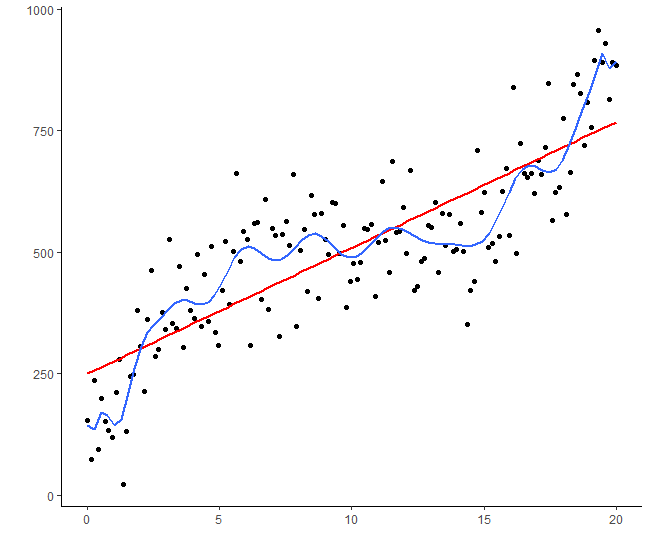
\includegraphics[scale=0.75]{./rys008}
\caption{Dopasowanie regresji liniowej (kolor czerwony) oraz wielomianu stopnia 25. (kolor niebieski) do danych opisanych za pomocą wzoru $500 + 0.4 * (x-10)^3 + \varepsilon$. \textit{Źródło:} opracowanie własne}\label{rys008}
\end{figure}


Błąd spowodowany wariancją jest wartością, o jaką funkcja celu się zmieni, jeśli użyjemy innego zbioru uczącego. Jeśli funkcja ta nie zmienia się znacząco dla różnych zbiorów danych, jesteśmy w stanie wnioskować, że algorytm dobrze aproksymuje funkcję mapującą zmienne objaśniające i objaśnianą. Algorytmy, które mają tendencje do wysokiej wariancji są silnie związane z charakterystyką danych treningowych. Oznacza to, że specyfika zbioru uczącego wpływa na liczbę i rodzaj parametrów użytych to aproksymacji funkcji mapującej. Takim zachowaniem cechują się głównie nieparametryczne algorytmy uczenia maszynowego, posiadające wysoką elastyczność (zdolność do odkrywania złożonych wzorców), takie jak drzewa decyzyjne czy algorytm k-najbliższych sąsiadów. Przykład tego problemu przedstawiony jest na rysunku~\ref{rys008}. Widać, że użyty model (niebieski kolor) „zapamiętał” zbiór użyty do treningu, łącznie z zawartym w danych szumem. Takie zjawisko jest znane jako nadmierne dopasowanie do danych (ang.~\textit{over-fitting}).


Możemy więc stwierdzić, że walczenie z błędem spowodowanym przez obciążenie bądź wariancję sprowadza się do zapobiegania sytuacji skrajnych w dopasowywaniu danych przez model. Obciążenie ulega zmniejszeniu, natomiast wariancja wzrasta w relacji ze złożonością modelu. Szczegółowiej, im więcej parametrów jest dodawanych do modelu, tym złożoność modelu jest większa, a wariancja staje się głównym problemem, podczas gdy obciążenie maleje. Przykładowo, dopasowując regresję wielomianową o coraz wyższych potęgach do danych widocznych na rysunku~\ref{rys008} rezultatem będzie lepsze dopasowanie krzywej do danych, kosztem większego ryzyka przeuczenia modelu. 

Rysunek~\ref{rys006} przedstawia graficzną zależność pomiędzy obciążeniem i wariancją, w stosunku do złożoności modelu i błędu. Zrozumienie tych dwóch głównych składowych błędu jest kluczowe do zrozumienia zachowania modeli predykcyjnych. W praktyce jednak, kryterium które brane jest pod uwagę to całkowity błąd, a nie jego dekompozycja. Niemniej jednak optymalną złożonością modelu jest taki punkt, dla którego wzrost obciążenia odpowiada spadkowi wariancji. Matematycznie możemy to zapisać jako:

\begin{equation} \label{wzor9g}
\frac{\partial obciazenie}{\partial zlozonosc\,  modelu} = -\frac{\partial wariancja}{\partial zlozonosc\,  modelu}
\end{equation}

\begin{figure}
\centering
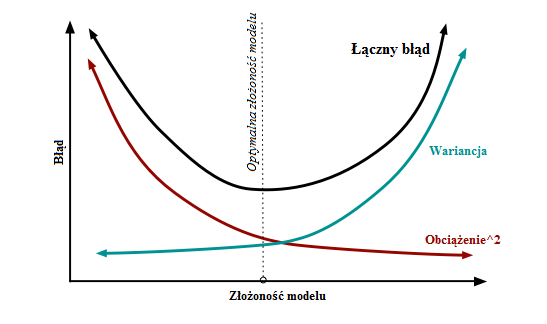
\includegraphics[scale=0.95]{./rys006}
\caption{Wizualizacja problemu optymalnej złożoności modelu. \textit{Źródło:} opracowanie własne}\label{rys006}
\end{figure}

Jeśli złożoność algorytmu przekracza ten punkt jesteśmy podatni na przeuczenie modelu. W przeciwnym razie istnieje ryzyko niedouczenia modelu. W praktyce nie da się w analityczny sposób znaleźć tego optymalnego punktu. Zamiast tego możemy dla różnych poziomów złożoności mierzyć błąd predykcji i wybierać taki, który minimalizuje łączny błąd. Kluczowe jest jednak dobranie odpowiedniej miary błędu, ponieważ ciężko jest posługiwać się błędem otrzymanym wyłącznie na zbiorze treningowym. Zamiast tego można posłużyć się technikami walidacji krzyżowej \citep{kohavi1995}.


\section{Optymalny klasyfikator bayesowski}

W przypadku tego klasfikatora, każda hipoteza $h(x)$ definiowana jest jako prawdopodobieństwo warunkowe. Dla nowej obserwacji $x$ i zbioru treningowego $T$, predykcja klasy i zmiennej zależnej $y$ może być postrzegane jako problem obliczenia następującego wyrażenia $p(y_i |T, x)$. Zapisując je jako ważona suma po wszystkich hipotezach w przestrzeni otrzymujemy:

\begin{equation} \label{wzor10}
p(y_i|T, x) = \sum_{h \in H} h(x)p(h| T)
\end{equation}


Wzór~\ref{wzor10} może być postrzegany jako klasyfikacja kombinowana składająca się ze wszystkich hipotez w zbiorze $H$, ważona prawdopodobieństwem a posteriori $p(h| T)$. Zgodnie z twierdzeniem Bayesa, prawdopodobieństwo to jest proporcjonalne do iloczynu prawdopodobieństwa wylosowania zbioru treningowego pod warunkiem prawdziwości hipotezy $h$  oraz prawdopodobieństwa \textit{a priori} hipotezy $h$ ($p(T| h)p(h)$). W niektórych przypadkach jesteśmy w stanie policzyć wszystkie składowe równiania~\ref{wzor10}. W takim przypadku żaden zbiór klasyfikatorów nie jest w stanie mieć lepszej predykcji niż klasyfikator bayesowski \citep{mitchell1977,hastie2009}.

Najcięższe do oszacowania a priori jest przekonanie o prawdziwości hipotezy $h$ ($p(h)$). Jeśli uda nam się w tym prawdopodobieństwie uchwycić całą wiedzę jaką mamy na temat funkcji f, wtedy z definicji nie jesteśmy w stanie już bardziej poprawić działania klasyfikatora. W praktyce jednak ciężko jest przypisać prawdopodobieństwo $p(h)$. Często ta wartość, razem z przestrzenią hipotez $H$ są dobierane tak, aby ułatwić obliczenia, jednak są one niepoprawne. W takim przypadku klasyfikator Bayesowski nie jest optymalny, a inne zbiory klasyfikatorów mogą prezentować większą zdolność predykcyjną.


\section{Bagging}

Algorytm Bagging (ang.~\textit{Bootstrap aggregating}) jest techniką pozwalającą na zmniejszenie wariancji modelu \citep{breiman1996}, używaną np. algorytmie lasów losowych (patrz podrozdział 2.2.2). Różnorodność klasyfikatorów otrzymywana jest poprzez stosowanie bootstrapowej próby z oryginalnego zbioru danych (losujemy obserwacje ze zbioru treningowego ze zwracaniem). Każdy podpróba używana jest do treningu osobnego modelu tego samego typu. Następnie, pojedyncze modele są łączone poprzez głosowanie większościowe. Dla każdej nowej obserwacji, klasa, która została wybrana przez większość modeli jest decyzją zbiorową. Jako że wylosowane zbiory treningowe mogą w znacznym stopniu się pokrywać, w celu zwiększenia różnorodności można budować klasyfikatory tylko na pewnej frakcji oryginalnego zbioru danych. Schemat działania algorytmu bagging został przedstawiony na poniższym schemacie.

\begin{algorithm}
\renewcommand\thealgorithm{}
\caption{Bagging}
\begin{algorithmic} \label{schemat2}
\STATE \textbf{Faza uczenia}
\STATE  $D \in \emptyset$, gdzie $D$ jest zbiorem klasyfikatorów
\STATE $L$, liczba klasyfikatorów użyta do treningu
\FOR{$k = 1, ..., L$}
\STATE Wylosuj bootstrapową próbę $S_k$ ze zbioru treningowego
\STATE Zbuduj klasyfikator $D_k$ używają próby $S_k$
\STATE Dodaj klasyfikator do istniejącego zbioru $D$ ($D = D \cup D_k$)
\ENDFOR  
\RETURN $D$

\STATE \textbf{Faza klasyfikacji}
\STATE Użyj danych wejściowych $x$ do klasyfikatorów $D_1, ..., D_L$
\STATE Klasa, która zebrała najwięcej głosów pośród klasyfikatorów zostaje wybrana
\end{algorithmic}
\addtocounter{algorithm}{-1}
\end{algorithm}

Załóżmy, że mamy do dyspozycji zbiór danych $(x_i, y_i)$ niezależnie wylosowanych z prawdziwej populacji $P$ o rozmiarze $N$ ($i = 1, ..., N$), gdzie $x$ jest wektorem zmiennych objaśniających, a $y$ wektorem zmiennej celu. Ponadto niech $y$ będzie zmienną numeryczną (ciągłą). W takim przypadku predykcję dla jednej bootstrapowej próby możemy zapisać jako $\hat{f^{*}}(x)$ . Tutaj $x$ jest stałe, natomiast próba składa się z obserwacji $(x_i^*, y_i^*)$, gdzie $i = 1, …, N$ jest wylosowane z rozkładu $P$. Dla takiej sytuacji możemy zapisać zagregowaną predykcję wielu modeli jako:
\begin{equation} \label{wzor11}
\hat{f}_{agreg}(x) = \frac{1}{N} \sum_{i = 1}^{N}\hat{f}(x_i)
\end{equation}

Następnie możemy zapisać błąd średniokwadratowy jako:
\begin{equation} \label{wzor12}
\frac{1}{N} \sum_{i = 1}^{N} (y_i - \hat{f}(x_i))^2 = y^2 - 2y\frac{1}{N} \sum_{i = 1}^{N} \hat{f}(x_i) + \frac{1}{N}\sum_{i = 1}^{N}\hat{f}(x_i)^2
\end{equation}

Korzystając z $\frac{1}{N}\sum_{i = 1}^{N}\hat{f}(x_i) = \hat{f}_{agreg}$ oraz $\mathbf{E}X^2 \geq (\mathbf{E}X)^2$ i podstawiając do wzoru \ref{wzor12} otrzymujemy:

\begin{equation} \label{wzor13}
\frac{1}{N}\sum_{i = 1}^{N}(y_i - \hat{f}(x_i))^2 \geq (y - \hat{f}_{agreg}(x))^2
\end{equation}

Po scałkowaniu obu stron równania~\ref{wzor13} po wspólnym rozkładzie zmiennych $x$ oraz $y$ otrzymujemy, że błąd średniokwadratowy $\hat{f}_{agreg}(x)$ jest niższy niż analogiczny błąd uśredniony dla budowanych pojedynczych modeli. To oznacza, że nawet używając modeli o niskiej skuteczności, jesteśmy w stanie w pewnym stopniu poprawić działanie poprzez zastosowanie baggingu. Należy jednak zaznaczyć, że tak zapisane oszacowanie zagregowanej predykcji nie jest wartością, którą moglibyśmy użyć w praktyce, jako że zakładamy losowanie z prawdziwej populacji $P$ (której zazwyczaj nie znamy). Ponadto należy zwrócić uwagę na stabilność poszczególnych modeli. Jeśli mamy do czynienia z niestabilnymi algorytmami, takimi jak drzewa decyzyjne czy sieci neuronowe, wtedy agregacja może przynieść pożądane skutki w postaci poprawy skuteczności. Używając jednak stabilnych modeli (np. algorytm K-najbliższych sąsiadów) bagging będzie najczęściej prowadzić do nieznacznego pogorszenia wyników \citep{hastie2009}. 

Zależność między stabilnością modelu a wynikiem \textit{baggingu} jest również spełniona w przypadku klasyfikacji (zmienna objaśniana jest kategoryczna). Ze względu jednak na nieaddytywność obciążenia i wariancji, użycie słabego klasyfikatora (gorszego niż losowe zgadywanie) będzie prowadzić do pogorszenia rezultatów w wyniku zastosowania algorytmu bagging (dowód oraz wyprowadzenie można znaleźć w artykule \citet{breiman1996}).

Ostatnim punktem, na który należy zwrócić uwagę jest utrata prostoty stosowanego modelu w procesie \textit{baggingu}. Przykładowo, starając się poprawić skuteczność drzew decyzyjnych używając tej techniki, wynikiem nie jest już drzewo. Jest to oczywista wada, jako że tracimy interpretowalność takiego algorytmu. Jak zostało wcześniej wspomniane, stosowanie bardziej stabilnych klasyfikatorów w baggingu zazwyczaj nie przynosi wymiernych korzyści w porównaniu z niestabilnymi. W tym drugim przypadku, niestabilność bierze się właśnie z położenia nacisku przy konstrukcji algorytmu na jego interpretowalność, a ta jest tutaj tracona. 

\section{Boosting}

Algorytm Boosting odnosi się do technik starających się przekształcić słabych uczniów (ang.~\textit{weak learners}) w modele o wysokiej mocy predykcyjnej. Słaby uczeń oznacza dokładnie klasyfikator, charakteryzujący się skutecznością nieznacznie wyższą niż losowe zgadywanie co do przynależności danego obiektu do konkretnej klasy. Czasami również zakłada się niską złożoność obliczeniową takiego ucznia. Robert Schapire w swoim artykule \citep{schapire1990} pokazał, że model potrafiący nieznacznie lepiej niż losowo dokonywać predykcji jest równie silny co algorytm popełniającym arbitralnie mały błąd. Dowód tej tezy oparł na takim filtrowaniu rozkładu prawdopodobieństwa, który pozwala słabemu uczniowi ostatecznie poznać prawie cały rozkład.

Większość algorytmów wykorzystujących idee boostingu składa się z sekwencyjnego uczenia słabych klasyfikatorów zgodnie z rozkładem prawdopodobieństwa, a następnie łączenia ich. Podczas łączenia, klasyfikatorom zostają przypisane wagi odzwierciedlające ich skuteczność. Po dodaniu słabego ucznia do komitetu modeli, wagi zostają zaktualizowane. Szczegółowiej, obserwacjom które zostały niepoprawnie sklasyfikowane zostaje zwiększona waga, a poprawnie zidentyfikowanym zmniejszana. Widać z tego, że kolejne budowane modele skupiają się bardziej na obserwacjach, na których wcześniej został popełniony błąd.

Dokładne działanie opisywanej techniki można zobrazować używając algorytmu AdaBoost (ang.~\textit{adaptive boosting}). Algorytm ten został zaproponowany w pracy \citep{freund1997} i był pierwszą techniką zbudowanym wokół idei boostingu. Rysunki~\ref{rys005a}, \ref{rys005b}, \ref{rys005c} przedstawiają kolejne iteracje działania modelu, podczas gdy rysunek \ref{rys005d} prezentuje końcową decyzję. W tym przypadku algorytm jako bazowego ucznia używa tzw. \textit{decision stump}, czyli drzewo decyzyjne składające się z korzenia połączonego bezpośrednio z liściami (inaczej mówiąc jest to jednopoziomowe drzewo decyzyjne). Wielkość obiektów przedstawionych na kolejnych rysunkach odpowiada wagom, jakie tym obserwacjom zostały przypisane. Dlatego też widzimy, że na początku działania algorytmu (rysunek~\ref{rys005a}) wszystkie wagi są sobie równe. W wyniku zastosowania jednopoziomowego drzewa została wygenerowana horyzontalna granica decyzyjna, niepoprawnie klasyfikująca część obiektów (przypisująca krzyżyki jako okręgi). Z tego powodu w kolejnej iteracji waga im odpowiadająca została zwiększona. To powoduje zmianę granicy decyzyjnej używając kolejnego klasyfikatora. Jak widać z rysunku~\ref{rys005b} spowodowało to, że obiekty te zostały prawidłowo przypisane, jednak nadal występuje błąd klasyfikacji. Z tego względu ponownie zwiększane są wagi dla obserwacji źle zaprognozowanych (dla instancji poprawnie przypisanych we wcześniejszych krokach waga ulega zmniejszeniu), a to skutkuje powstaniem nowej wertykalnej linii decyzyjnej (rysunek~\ref{rys005c}). Rysunek~\ref{rys005d} przedstawia złożoną regułę decyzyjną złożoną na podstawie 3 iteracji algorytmu. Widzimy, że takie połączenie pozwala na skuteczniejsze podzielenie klas ze zbioru treningowego, niż w przypadku użycia pojedynczych klasyfikatorów.

\begin{figure}[ht] 
  \begin{subfigure}[b]{0.5\linewidth}
    \centering
    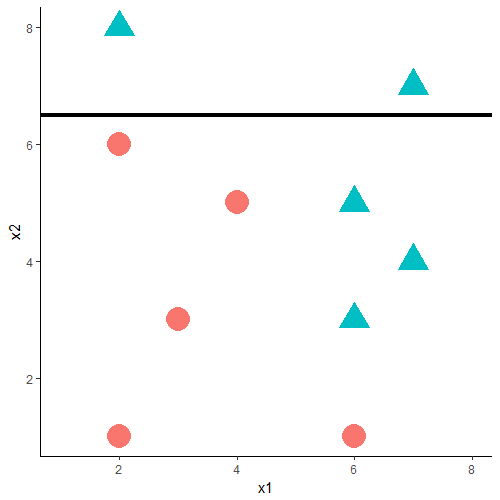
\includegraphics[width=0.75\linewidth]{./rys005a} 
    \caption{1. krok działania algorytmu} 
    \label{rys005a} 
    \vspace{4ex}
  \end{subfigure}%% 
  \begin{subfigure}[b]{0.5\linewidth}
    \centering
    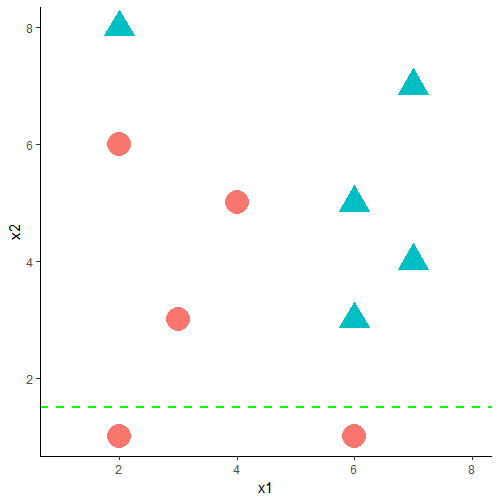
\includegraphics[width=0.75\linewidth]{./rys005b} 
    \caption{2. krok działania algorytmu} 
    \label{rys005b} 
    \vspace{4ex}
  \end{subfigure} 
  \begin{subfigure}[b]{0.5\linewidth}
    \centering
    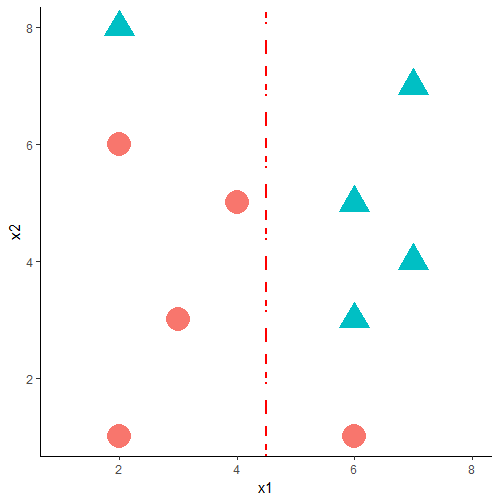
\includegraphics[width=0.75\linewidth]{./rys005c} 
    \caption{3. krok działania algorytmu} 
    \label{rys005c} 
  \end{subfigure}%%
  \begin{subfigure}[b]{0.5\linewidth}
    \centering
    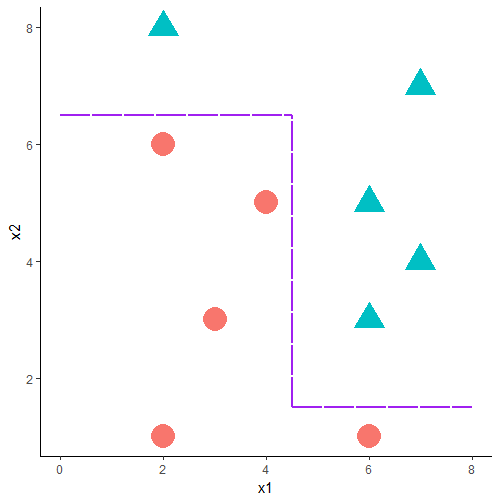
\includegraphics[width=0.75\linewidth]{./rys005d} 
    \caption{Decyzja końcowa} 
    \label{rys005d} 
  \end{subfigure} 
  \caption{Działanie algorytmu \textit{Boosting} na sztucznie wygenerowanych danych. \textit{Źródło:} opracowanie własne}
  \label{fig7} 
\end{figure}

W wyżej opisanym przypadku jako słabych uczniów użyliśmy jednopoziomowe drzewa decyzyjne. Generalnie jednak, każdy algorytm uczenia maszynowego może być użyty zgodnie z zasadą boostingu, pod warunkiem, iż pozwala na przypisanie wag poszczególnym obserwacjom ze zbioru danych. Innym stosowanym algorytmem wzmacniania jest XGBoost (patrz podrozdział 2.2.7) oraz Gradient Boosting \citep{friedman2001}.

Warto zwrócić uwagę, że mimo niewątpliwych zalet, algorytmy oparte na wzmacnianiu zostały poddawane krytyce w literaturze \citep{long2010}. Jako powód wadliwości tej techniki wskazywana słaba wytrzymałość w stosunku do obecności szumu w danych. Co za tym idzie poddawana wątpliwości jest zdolność jej zastosowania w rzeczywistych problemach. Wymieniony artykuł pokazuje, że jeśli w danych znajduje się jakaś część niepoprawnie zaklasyfikowanych (np. w wyniku błędu ludzkiego), wtedy algorytm \textit{boostingu} w wyniku kolejnych iteracji stara się je poprawnie przypisać, jednak powoduje to niemożność osiągnięcia skuteczności wyższej niż 0.5 (w przypadku klasyfikacji binarnej). Jako przykładowy algorytm wpadający w tą pułapkę został wskazany AdaBoost, niemniej jednak autor sugeruje możliwość występowania modeli tolerujących takie zniekształcenia w danych.

\section{Stacking}

Kontaminacja modeli (ang.~\textit{stacking}, \textit{stacked generalization}) jest techniką klasyfikacji kombinowanej polegającą na łączeniu informacji pochodzących z wielu algorytmów predykcyjnych, w celu zbudowania nowego modelu. W przeciwieństwie do \textit{baggingu} czy \textit{boostingu}, stacking łączy modele uczenia maszynowego różnych rodzajów. W wielu przypadkach używanie kontaminacji modeli daje lepsze rezultaty niż stosowanie osobno pojedynczych algorytmów ze względu na zdolność skupiania się na mocnych aspektach modeli i niwelowaniu słabych \citep{wolpert1992}. Z tego względu metoda staje się efektywna, kiedy bazowe modele różnią się między sobą w znaczącym stopniu.

Schemat budowania kontaminacji modeli możemy przedstawić w następujących krokach:
\begin{enumerate}
\item Niech wejściowy zbiór treningowy $X$ składa się z $n$ obserwacji oraz $k$ zmiennych objaśniających
\item Na podstawie zbioru $X$ uczone jest $M$ modeli bazowych
\item Każdy model generuje predykcję zmiennej objaśnianej $y$, które następnie zbierane są do jednej macierzy $X_2$ (macierz ta będzie wymiarów $n x M$)
\item Dane zawarte w macierzy $X_2$ służą do wytrenowania modelu drugiego poziomu, pozwalającego na predykcję na zbiorze testowym
\end{enumerate}
Graficzna reprezentacja jest także widoczna na rysunku~\ref{rys007}.

W powyższym postępowaniu należy zwrócić uwagę na budowanie macierzy $X_2$. Gdybyśmy do wytrenowania modeli bazowych $M$ użyli wszystkich rekordów ze zbioru $X$, wtedy model drugiego poziomu byłby obciążony w stosunku do najlepszego modelu spośród wszystkich bazowych. Takie zjawisko nosi nazwę wycieku danych (ang.~\textit{data leakage}) i oznacza nieprzewidywane stworzenie dodatkowej informacji do zbioru treningowego, skutkujące w tworzeniu nierealistycznie dobrych predykcji. Rozwiązaniem tego problemu jest zastosowanie k-krotnej walidacji krzyżowej. Dzięki temu w kolejnych iteracjach walidacji będziemy uzupełniać macierz $X_2$ predykcjami, które nie brały udziały w procesie trenowania modeli bazowych (ang.~\textit{out-of-sample predictions}).

Ważną kwestią pozostaje dobór odpowiedniego modelu łączącego. W przypadku regresji zostało udowodnione, że metoda najmniejszych kwadratów spisuje się do tego zadania odpowiednio \citep{breiman1996b}. Szczegółowiej, jako modele bazowe zostały wykorzystane drzewa regresyjne o różnym rozmiarze, a także modele regresji liniowej z różną ilością zmiennych decyzyjnych. W celu predykcji na podstawie modelów pierwszego stopnia użyto ponownie regresji liniowej, jednak z ograniczenie, że wszystkie parametry modelu muszą być nieujemne. Warunek ten okazał się kluczowy w celu zapewnienia poprawy zdolności predykcyjnej w stosunku do pojedynczych modeli. 

\citet{ting1999} rozszerzyli pracę Breimana na przypadek klasyfikacji. Ich wyniki potwierdziły skuteczność modeli liniowych jako generalizatorów wiedzy, zaznaczając przy tym jednocześnie że warunek nieujemności parametrów w nieznaczącym stopniu przyczynia się do poprawy skuteczności modelu. Ponadto zastosowanie regresji liniowej zwiększa interpretowalność otrzymanych wyników – wielkość parametrów określa udział każdego modelu bazowego w predykcji prawdopodobieństwa przynależności do konkretnej klasy (zastosowanie warunku nieujemności ułatwia interpretacje, sprowadzając się do tego jak dany model przyczynia się do predykcji danej klasy). Jak jednak okazuje się, pomimo niewątpliwych zalet modele liniowe nie wykorzystują w pełni potencjału zawartego w metazmiennych (predykcji modeli bazowych), które mogą zawierać bardziej złożone zależności ze zmienną celu \citep{sill2009}. Dlatego też w literaturze można spotkać przykłady zastosowania nieliniowych metod uczenia maszynowego, takich jak sieci neuronowe czy boosting drzew decyzyjnych \citep{moudrik2015}.

Ze względu na swoją strukturę, stacking jest metodą czasochłonną obliczeniowo, a w przypadku używania nieliniowych modeli łączących również nieinterpretowalną. Jednak kiedy czas i zasoby nie odgrywają ważnej roli w rozwiązywaniu konkretnego problemu, może okazać się że technika ta jest bardzo pomocna. W istocie, kiedy analizowany problem jest złożony, naturalnym wydaje się powstawanie różnych koncepcji modelowania zjawiska (doboru zmiennych, transformacji, modelu czy hiperparametrów). Jeśli głównym celem takiego badania jest skuteczność modeli, w takiej sytuacji dobrym pomysłem może okazać się \textit{stacking}. 

Przykładem takiego postępowania są konkursy analiz danych organizowane na serwisach internetowych (np. \url{kaggle.com}, \url{drivendata.org}), w których użytkownicy starają się rozwiązywać stawiane problemy, m.in. z użyciem technik uczenia maszynowego. Jeden z najpopularniejszych konkursów dotyczył poprawy systemu rekomendującego użytkownikom serwisu Netflix seriale i filmy do obejrzenia. Trwał on prawie 3 lata i przyczynił się do rozwoju wielu narzędzi, nie tylko systemów rekomendacyjnych, ale także modeli predykcyjnych \citep{bell2007,bennett2007}. Ponadto okazuje się, że drużyny, które zajęły najwyższe miejsca w rankingu, używały metody stackingu do swoich ostatecznych predykcji \citep{jahrer2010}. Były to jednak o wiele bardziej złożone struktury, niż te opisane wcześniej, zawierające kilka warstw iteracyjnego łączenia modeli \citep{toscher2009}.

\begin{figure}
\centering
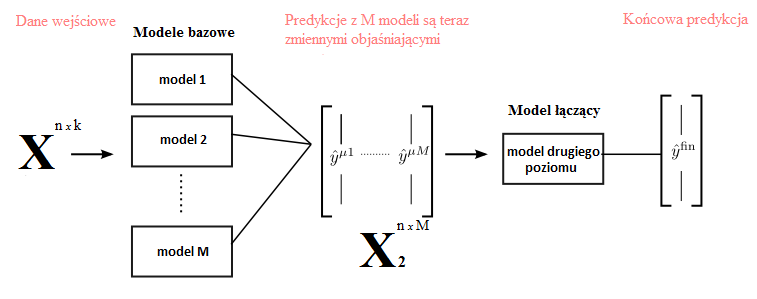
\includegraphics[scale=0.85]{./rys007}
\caption{Schemat działania \textit{stackingu}. \textit{Źródło:} opracowanie własne}\label{rys007}
\end{figure}

\section{Reguły kombinacyjne}

Poza wyżej wymienionymi technikami, możliwe jest także łączenie wyników z różnych modeli w prostszy sposób. Po zakończeniu fazy uczenia algorytmów uczących, czy to za pomocą metod walidacji krzyżowej, czy też używając do tego całości zbioru treningowego, dokonujemy prognozy na zbiorze wcześniej niewidzianym przez konkretne modele. W przypadku klasyfikacji, wynikiem takiej prognozy mogą być prawdopodobieństwa przynależności obiektu do wskazanej klasy, bądź też od razu wynikowa klasa (po ustaleniu progu odcięcia). W obu przypadkach możliwe jest połączenie tych wyników za pomocą algebraicznych reguł, bez konieczności dodatkowej fazy uczenia (ang.~\textit{non-trainable combiners}).

Załóżmy, że zostało zbudowanych $M$ modeli bazowych, a zmienna objaśniana ma $K$ klas. W takim przypadku decyzja o przynależności do $k$ klasy w modelu $m$ może być zapisana jako $d_{m, k} \in \{0, 1\}$, gdzie $m = 1, ..., M$ oraz $k = 1, ..., K$. Możemy też zapisać prawdopodobieństwo przynależności jako $p_{m, k} \in {[0,1]}$. Ostateczną decyzją będzie taka klasa $k$, która otrzymała najwyższą wartość wyrażenia $\mu_k$ oznaczającego zastosowanie konkretnej reguły kombinacyjnej na tej klasie. Oznaczając jako $d_{final}$ końcową decyzje możemy zapisać:

\begin{equation} \label{wzor14}
d_{final}(x) = \argminl_{k}\mu_k(x)
\end{equation}

Reguły kombinacyjne dla poszczególnych klas można zapisać w następujący sposób:
\begin{itemize}
\item Reguła średniej: $\mu_k(x) = \frac{1}{M}\sum_{m = 1}^{M}p_{m, k}(x)$
\item Reguła średniej ważonej: $\mu_k(x) = \sum_{m = 1}^{M}w_mp_{m, k}(x)$, gdzie $w_m$ oznacza wagę przypisaną do klasyfikatora $m$, np. na podstawie jego skuteczności na zbiorze treningowym
\item Reguła maksimum: $\mu_k(x) = \max_{m = 1, ..., M}\{p_{m, k}(x)\}$
\item Reguła minimum: $\mu_k(x) = \min_{m = 1, ..., M}\{p_{m, k}(x)\}$
\item Reguła mediany: $\mu_k(x) = \mathrm{median}_{m = 1, ..., M}\{p_{m, k}(x)\}$
\item Głosowanie większościowe $\mu_k(x) = \sum_{m = 1}^{M} d_{m, k}(x)$
\end{itemize}

\chapter{Metodologia oraz wyniki}

Rozdział zawiera opis przygotowania danych zawierających notowania spółek notowanych na Giełdzie Papierów Wartościowych na potrzeby klasyfikacji kierunku przyszłych zmian cen. Ponadto przedstawione są wyniki skuteczności użytych algorytmów uczenia maszynowego, a także ich łączenia za pomocą reguł kombinacyjnych oraz kontaminacji.

\section{Przygotowanie danych}
Dane użyte w pracy zostały pobrane z oficjalnej strony Giełdy Papierów Wartościowych w Warszawie (\url{https://www.gpw.pl/notowania_archiwalne}). Zawierają notowania spółek notowanych na warszawskim parkiecie od 16 kwietnia 1991 (pierwsza sesja giełdowa) roku do 10 marca 2017, a także wartości wszystkich dostępnych indeksów (m.in. indeksy największych spółek, sektorowe czy narodowe) za analogiczny okres. W przypadku akcji dla każdej spółki zostały wyciągnięte również dane na temat kursu otwarcia i zamknięcia, maksymalnej oraz minimalnej wartości w przeciągu sesji, wolumenie transakcji, a także wartości obrotu. Te same zmienne zostały również pobrane dla indeksów. Wszystkie dane zostały zapisane w postaci dwóch baz danych SQLite, pozwalających na wykonywanie zapytań za pomocą języka SQL. Przykładowe wycinki danych dla akcji i indeksów przedstawia tabela~\ref{tab001} oraz~\ref{tab002}.

\begin{table}[ht] 
\caption{Losowo wybrane obserwacje z oryginalnego zbioru danych dla notowanych spółek. \textit{Źródło:} \protect\url{https://www.gpw.pl/notowania_archiwalne}}\label{tab001}
\centering
\resizebox{\textwidth}{!}{\begin{tabular}{llllrrrrrrrr}
  \hline
data & nazwa & ISIN & waluta & otwarcie & maksimum & minimum & zamkniecie & zmiana\_kursu & wolumen & transakcje & wartosc\_obrotu \\ 
  \hline
2013-02-27 & CAPITAL & PLCPTLP00015 & PLN & 1.38 & 1.38 & 1.29 & 1.36 & 4.62 & 5883.00 & 27.00 & 7.77 \\ 
  2013-11-08 & MILLENNIUM & PLBIG0000016 & PLN & 7.20 & 7.39 & 7.06 & 7.21 & -0.69 & 1086081.00 & 350.00 & 7727.77 \\ 
  2004-06-02 & PROKOM & PLPROKM00013 & PLN & 181.00 & 187.00 & 181.00 & 185.00 & 2.49 & 20859.00 & 231.00 & 7737.95 \\ 
  2003-09-29 & EFL & PLEFL0000016 & PLN & 51.20 & 54.00 & 51.20 & 53.50 & 0.00 & 813.00 & 17.00 & 86.90 \\ 
  2015-08-10 & WESTAISIC & LU0627170920 & PLN & 0.00 & 0.00 & 0.00 & 0.08 & 0.00 & 0.00 & 0.00 & 0.00 \\ 
  1999-04-07 & MILLENNIUM & PLBIG0000016 & PLN & 8.85 & 9.00 & 8.60 & 8.85 & 2.90 & 3656330.00 & 290.00 & 36566.90 \\ 
  2003-04-23 & KOMPAP & PLKOMPP00017 & PLN & 4.85 & 5.00 & 4.75 & 5.00 & -0.99 & 1002.00 & 6.00 & 9.64 \\ 
  2016-10-20 & AGORA & PLAGORA00067 & PLN & 10.58 & 10.60 & 10.53 & 10.58 & 0.00 & 23893.00 & 44.00 & 252.38 \\ 
  2012-01-17 & COGNOR & PLCNTSL00014 & PLN & 3.32 & 3.65 & 3.32 & 3.65 & 9.94 & 145929.00 & 162.00 & 524.37 \\ 
  2013-02-22 & NFIEMF & PLNFI1500011 & PLN & 18.54 & 18.83 & 18.54 & 18.83 & 1.51 & 164.00 & 11.00 & 3.08 \\ 
   \hline
\end{tabular}}
\end{table}


\begin{table}[ht] 
\caption{Losowo wybrane obserwacje z oryginalnego zbioru danych dla notowanych indeksów. \textit{Źródło:} \protect\url{https://www.gpw.pl/notowania_archiwalne}}\label{tab002}
\centering
\resizebox{\textwidth}{!}{\begin{tabular}{llllrrrrrrrr}
  \hline
data & nazwa & ISIN & waluta & otwarcie & maksimum & minimum & zamkniecie & zmiana\_kursu & wolumen & transakcje & wartosc\_obrotu \\ 
  \hline
2013-04-23 & WIG-PLUS & PL9999999441 &  & 775.91 & 776.29 & 765.99 & 769.16 & -0.93 & 0.00 & 0.00 & 9614.61 \\ 
  2013-11-25 & WIG-DEWEL & PL9999999706 &  & 1618.26 & 1618.61 & 1617.11 & 1618.61 & 0.05 & 0.00 & 0.00 & 11032.75 \\ 
  2005-06-08 & WIG-BANKI & PL9999999904 & PLN & 3749.51 & 3767.54 & 3749.51 & 3767.54 & 0.22 & 0.00 & 0.00 & 340921.81 \\ 
  2004-10-21 & NIF & PL9999999961 & PLN & 81.63 & 82.62 & 81.05 & 82.62 & 0.01 & 0.00 & 0.00 & 1412.87 \\ 
  2015-07-27 & WIG-BANKI & PL9999999904 &  & 6468.95 & 6516.00 & 6468.95 & 6516.00 & -0.94 & 0.00 & 0.00 & 259560.81 \\ 
  1999-07-08 & WIG-SPOZYW & PL9999999888 & PLN & 1530.20 & 1530.20 & 1530.20 & 1530.20 & -0.17 & 0.00 & 0.00 & 0.00 \\ 
  2004-05-13 & WIG-BUDOW & PL9999999896 & PLN & 1845.75 & 1845.75 & 1832.66 & 1834.01 & -0.56 & 0.00 & 0.00 & 9236.67 \\ 
  2016-11-17 & INVESTORMS & PL9999999672 &  & 4099.15 & 4099.15 & 4090.50 & 4090.50 & -0.36 & 0.00 & 0.00 & 246883.34 \\ 
  2012-04-30 & WIG-INFO & PL9999999771 &  & 1119.87 & 1119.87 & 1116.58 & 1118.09 & 0.99 & 0.00 & 0.00 & 9969.82 \\ 
  2013-04-19 & TBSP.INDEX & PL9999999474 &  & 1503.45 & 1505.98 & 1503.45 & 1505.98 & 0.08 & 0.00 & 0.00 & 0.81 \\ 
   \hline
\end{tabular}}
\end{table}

Łączna liczba dostępnych obserwacji dla akcji wynosiła 1 623 715. Pierwszym problemem, jaki się pojawił był brak cen otwarcia, maksymalnej oraz minimalnej dla sesji giełdowych z początku działania GPW. Jako, że niektóre używane w dalszej części zmienne objaśniające potrzebują tych danych do kalkulacji, zdecydowano o usunięciu tych rekordów. Kolejnym krokiem było odfiltrowanie spółek, których debiut nastąpił po 1 stycznia 2016 roku. Miało to na celu pozbycie się obserwacji, które przy tworzeniu nowych zmiennych (korzystających ze wcześniejszych notowań) mogłyby generować braki w danych. Ponadto notowania spółek o krótkim stażu na giełdowym parkiecie wykazują tendencję do bycia niewłaściwie wycenianymi przez inwestorów \citep{purnanandam2004}, co mogłoby skutkować obciążeniem końcowego modelu.

W przypadku indeksów nie była konieczna podobna filtracja danych. Jak jednak sugeruje m.in.~\citet{madge2015}, do predykcji kierunku cen akcji użyteczne mogą być informację zawarte w notowaniach indeksów, do których należą. Szczegółowiej, zostało udowodnione, iż zastosowanie ich w modelach predykcyjnych pozwala lepiej oddać całościową sytuację występującą na rynku \citep{swensen2015,citak2007}. Indeksy skupiające spółki z tych samych sektorów charakteryzują się na polskim parkiecie w wielu przypadkach niewielką liczebnością oraz niskim średnim obrotem (tabela~\ref{tab003}). Niski obrót na instrumentach powoduje niewielką płynność, co może doprowadzić do manipulacji kursem przez pojedynczych inwestorów \citep{allen1992}. Dlatego też zdecydowano o wybraniu do dalszej analizy tylko spółek wchodzących w skład indeksu WIG20, czyli 20 największych przedsiębiorstw notowanych na GPW, pod względem wartości obrotu oraz kapitalizacji rynkowej. Skład spółek wchodzących w skład tego indeksu został wybrany na 10 marca 2017. 

\begin{table}[ht] 
\caption{Liczebność i średnia wartość obrotu dla dostępnych indeksów sektorowych oraz indeksu WIG20. Skład indeksów na 10 marca 2017. \textit{Źródło:} Opracowanie własne}\label{tab003}
\centering
\begin{tabular}{lrr}
  \hline
Indeks & Średnia wart. obrotu & Liczebność \\ 
  \hline
WIG-GORNIC & 47839.99 & 5.00 \\ 
  WIG20 & 39444.86 & 20.00 \\ 
  WIG-BANKI & 24494.51 & 14.00 \\ 
  WIG-PALIWA & 21818.47 & 9.00 \\ 
  WIG-ENERG & 8130.88 & 10.00 \\ 
  WIG-LEKI & 5776.27 & 6.00 \\ 
  WIG-CHEMIA & 2954.73 & 7.00 \\ 
  WIG-MEDIA & 1477.87 & 12.00 \\ 
  WIG-NRCHOM & 1451.35 & 30.00 \\ 
  WIG-ODZIEZ & 1144.32 & 21.00 \\ 
  WIG-INFO & 1017.50 & 23.00 \\ 
  WIG-BUDOW & 837.75 & 45.00 \\ 
  WIG-MOTO & 750.56 & 7.00 \\ 
  WIG-SPOZYW & 543.45 & 26.00 \\ 
   \hline
\end{tabular}
\end{table}

Zmienne objaśniające użyte w modelowaniu zawierały zmienność oraz momentum (średnia zmiana kierunku ceny w przeciągu n ostatnich dni) wyliczone zarówno dla spółek, jak i indeksów. Zmienne te były sparametryzowane pod względem ilości dni używanych do kalkulacji. Ponadto,  użyte zostały wskaźniki analizy technicznej, takie jak wskaźnik względnej siły (ang. Relative Strength Index, RSI), indeks kanału towaru (ang. Commodity Channel Index, CCI), wskaźnik akumulacji i dystrybucji Williamsa (ang. Williams Accumulation/Distribution Indicator, WilliamsAD) czy wskaźnik zmiany (ang. Rate of Change, ROC), których zdolności predykcyjne przy konstruowaniu strategii inwestycyjnych zostały udowodnione w literaturze \citep{patel2015}. Parametry użyte do wskaźników stanowiły standardowe ustawienia przyjęte w literaturze \citep{murphy1999}. Dokładny opis użytych parametrów zawiera tabela~\ref{tab004}.

\begin{table}[ht] 
\caption{Ustawienia parametrów we wskaźnikach analizy technicznej użytych w pracy. \textit{Źródło:} Opracowanie własne}\label{tab004}
\centering
\begin{tabular}{lrr}
  \hline
Wskaźnik & Nazwa paramteru & Wartość\\ 
  \hline
Relative Strength Index (RSI) & Liczba okresów średniej ruchomej & 14 \\
Rate of Change (ROC) & Liczba dni użytych do kalkulacji & 10 \\
Commodity Channel Index (CCI) & Liczba okresów średniej ruchomej & 14 \\
Williams Accumulation/Distribution & - & - \\
  \hline
\end{tabular}
\end{table}

Jak zostało wcześniej wspomniane, zmienną objaśnianą w pracy jest zmiana kierunku ceny. Notowanie spółki może w odniesieniu do przyjętej wartości odniesienia wzrosnąć, spaść, bądź nie zmienić ceny. Tabela~\ref{tab005} przedstawia jak rozkładała się zmiana ceny dla wszystkich spółek w badanym okresie. Widzimy, że przypadek, kiedy w danym okresie cena nie zmienia swej wartości stanowi tylko 14.74\% wszystkich przypadków. Stosując do dalszej analizy taki podział zmiennej objaśnianej mielibyśmy do czynienia z problemem, tzw. niezbilansowanej próby (ang. imbalanced classification problem). Taka sytuacja mogłaby prowadzić do ignorowania przez zbudowany klasyfikator jednej klasy podczas predykcji, co miałoby przełożenie w skuteczności stosowanej metody \citep{he2009}. Przykładowo załóżmy, że mamy do dyspozycji zbiór danych, w którym zmienna objaśniana jest na skali dychotomicznej, a jej jedna klasa stanowi 90\% wszystkich przypadków. W takiej sytuacji klasyfikator nauczony na takich danych mógłby wykazywać skuteczność na poziomie ok. 90\%. Tak dobry wynik nie wynikałby jednak z poprawnie odczytanych wzorców, lecz z dokonywania prognoz tylko nadreprezentowanej klasy. Z tego względu, w celu uniknięcia takiej sytuacji dokonano połączenia przypadku braku zmiany kwotowań razem ze wzrostem.

\begin{table}[ht] 
\caption{Liczba przypadków kierunku zmiany cen akcji. \textit{Źródło:} Opracowanie własne}\label{tab005}
\centering
\begin{tabular}{lrr}
  \hline
Zmiana ceny & Liczba przypadków \\
  \hline
Wzrost & 383 466\\
Spadek & 419 123\\
Bez zmian & 138 713\\
  \hline
\end{tabular}
\end{table}

Ponadto użyto różnych okien prognozy, w celu sprawdzenia skuteczności technik klasyfikacji kombinowanej w zależności od czasu. Również używane były różne kombinacje parametrów do obliczania zmienności i momentum dla akcji i indeksów. Dlatego też cały schemat przepływu danych (ang.~\textit{data flow}) przez różne algorytmy uczenia maszynowego odbywał się niezależnie dla kolejnych kombinacji tych trzech parametrów. Należy zwrócić uwagę, iż parametry przy wskaźnikach analizy technicznej zostały na stałym poziomie niezależnie od okna prognozy i ilości dni użytych do kalkulacji pozostałych zmiennych. Wykaz użytych parametrów przedstawiony został w tabeli~\ref{tab006}.

\begin{table}[ht] 
\caption{Kombinacje parametrów (do zmiennych objaśniających używających notowań akcji i indeksów), oraz okien prognozy użytych w pracy. \textit{Źródło:} Opracowanie własne}
\label{tab006}
\centering
\begin{tabular}{lrr}
  \hline
Akcje & Indeksy & Okno prognozy \\
  \hline
10 & 5 & 1 \\ 
  20 & 5 & 1 \\ 
  90 & 5 & 1 \\ 
  10 & 10 & 1 \\ 
  20 & 20 & 270 \\ 
  10 & 10 & 270 \\ 
  5 & 5 & 270 \\ 
  270 & 270 & 90 \\ 
  90 & 90 & 90 \\ 
  20 & 20 & 90 \\ 
  10 & 10 & 90 \\ 
  5 & 5 & 90 \\ 
  270 & 270 & 20 \\ 
  90 & 90 & 20 \\ 
  20 & 20 & 20 \\ 
  10 & 10 & 20 \\ 
  5 & 5 & 20 \\ 
  270 & 270 & 10 \\ 
  90 & 90 & 10 \\ 
  20 & 20 & 10 \\ 
  10 & 10 & 10 \\ 
  5 & 5 & 10 \\ 
  270 & 270 & 5 \\ 
  90 & 90 & 5 \\ 
  20 & 20 & 5 \\ 
  10 & 10 & 5 \\ 
  5 & 5 & 5 \\ 
  270 & 270 & 1 \\ 
  90 & 90 & 1 \\ 
  20 & 20 & 1 \\ 
   \hline
\end{tabular}
\end{table}

Po połączeniu danych zawierających zmienne na temat akcji oraz indeksów w jedną tabele oraz usunięciu brakujących obserwacji (rekordy początkowe, dla których policzenie wskaźników nie było możliwe) otrzymano końcowy zbiór danych. W celu użycia go do budowy różnych klasyfikatorów dokonano losowego podziału, w wyniku którego zbiór treningowy zawierał 60\%, a testowy 40\% całkowitej liczby obserwacji. Przykładowy wycinek końcowych danych przedstawiony jest w tabeli~\ref{tab007}.

\begin{table}[ht]
\caption{Losowo wybrane obserwacje z przetworzonego zbioru danych. \textit{Źródło:} Opracowanie własne}
\label{tab007}
\centering
\resizebox{\textwidth}{!}{\begin{tabular}{lrrrrrrrr}
  \hline
target & stock\_momentum & stock\_volatility & index\_momentum & index\_volatility & CCI & ROC & RSI & Williams \\ 
  \hline
wzrost & 0.24 & 0.00 & -0.07 & -0.00 & -92.73 & -0.02 & 46.64 & 1.29 \\ 
  spadek & 0.33 & 0.01 & 0.20 & 0.00 & 73.48 & 0.21 & 79.14 & 206.30 \\ 
  wzrost & 0.07 & -0.00 & -0.04 & -0.00 & 6.37 & -0.01 & 43.87 & 2.16 \\ 
  wzrost & 0.24 & 0.00 & 0.22 & 0.00 & -16.06 & -0.03 & 52.94 & 108.24 \\ 
  wzrost & 0.02 & 0.00 & -0.02 & -0.00 & -83.43 & -0.02 & 42.63 & 8.28 \\ 
  wzrost & 0.07 & 0.00 & -0.04 & -0.00 & -140.73 & -0.07 & 42.20 & -230.00 \\ 
  spadek & 0.44 & -0.00 & -0.11 & -0.00 & -270.53 & -0.06 & 23.16 & -0.03 \\ 
  wzrost & 0.18 & -0.00 & -0.02 & 0.00 & 93.04 & 0.05 & 66.83 & 15.96 \\ 
  spadek & -0.07 & 0.00 & 0.00 & -0.00 & -62.13 & -0.05 & 48.80 & 80.72 \\ 
  spadek & 0.16 & 0.01 & 0.16 & 0.00 & 126.75 & 0.01 & 62.61 & 10.61 \\ 
   \hline
\end{tabular}}
\end{table}

\section{Modelowanie}

Wszystkie bazowe algorytmy użyte w pracy zostały trenowane za pomocą 3-krotnej walidacji krzyżowej. Oznacza to, że dla każdej kombinacji hiperparametrów dostępnych w modelu, zbiór treningowy był dzielony losowo na 3 podzbiory. Następnie dwa z tych podzbiorów były łączone, by na nich dokonać procesu uczenia modelu. Na trzecim zbiorze dokonywana została predykcja klas. Proces ten był przeprowadzamy trzykrotnie, dzięki czemu byliśmy w stanie otrzymać nieobciążone prognozy dla całego zbioru treningowego. Dzięki temu na podstawie skuteczności (odsetek poprawnie zaklasyfikowanych przypadków) możliwy był wybór najlepszej kombinacji parametrów dla danego algorytmu uczenia maszynowego. Należy zwrócić uwagę, że w przypadku każdego algorytmu był używany ten sam podział zbioru podczas walidacji krzyżowej, tak aby umożliwić prawidłowe porównanie wyników.
W procesie budowy zespołu klasyfikatorów zostały użyte następujące algorytmy bazowe:
\begin{itemize}
\item algorytm kNN
\item drzewa decyzyjne zbudowane za pomocą algorytmu CART
\item bagging drzew decyzyjnych CART
\item lasy losowe
\item regresja logistyczna
\item liniowa analiza dyskryminacyjna
\item kwadratowa analiza dyskryminacyjna
\item metoda wektorów nośnych z różnymi funkcjami jądrowymi (liniowa, wielomianowa oraz gaussowska)
\item algorytm XGBoost
\item algorytm AdaBoost
\end{itemize}

W rozdziale drugim poruszana była kwestia kompromisu pomiędzy obciążeniem a wariancją modelu. Wynikała z niego konkluzja o istotności znalezienia optymalnej złożoności modelu w celu uniknięcia ryzyka przeuczenia i niedouczenia modelu. Dlatego też w pracy każdy algorytm (o ile było to możliwe) był budowany w różnych ustawieniach dostępnych parametrów. Listę użytych hiperparametrów przedstawia tabela~\ref{tab008}.

\begin{table}[ht] 
\caption{Kombinacje parametrów w algorytmach uczenia maszynowego użyte w pracy. \textit{Źródło:} Opracowanie własne}
\label{tab008}
\centering
\begin{tabular}{lcc}
  \hline
Algorytm & Parametry & Wartości \\
  \hline
kNN & Liczba sąsiadów & 3, 5, 10, 20, 30, 50, 100, 100 \\
CART & Złożoność & 20 różnych kombinacji \\
bagging CART & brak & brak \\
lasy losowe & \makecell{Liczba zmiennych losowana\\ do konstrukcji} & 1, 2, 3 \\
regresja logistyczna & brak & brak \\
LDA & brak & brak \\
QDA & brak & brak \\
SVM & Koszt & 4 różne kobinacje \\
XGBoost & \makecell{Liczba drzew, tempo uczenia,\\ procent losowanych wierszy\\ i kolumn} & 8 różnych kombinacji \\
AdaBoost & Liczba iteracji & 50, 100 \\
  \hline
\end{tabular}
\end{table}


Po zakończonym etapie uczenia modeli otrzymujemy wyniki oraz prawdopodobieństwa przynależności obserwacji do danej klasy na zbiorze treningowym. Dzięki temu możemy porównać skuteczność poszczególnych metod między sobą, a także zmienność skuteczności dla różnych parametrów w obrębie jednego algorytmu. Przykładowe porównanie wyników za pomocą wykresu pudełkowego dla dwóch wybranych okien prognozy zostały przedstawione na rysunkach~\ref{rys010a} oraz~\ref{rys010b}.

\begin{figure}
\centering
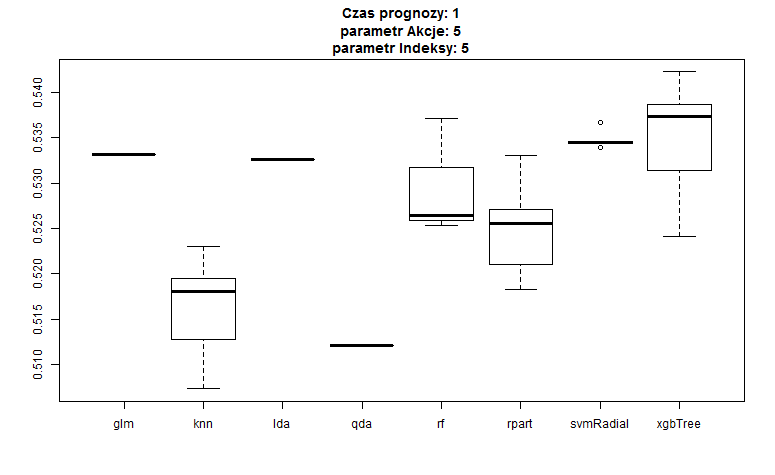
\includegraphics[scale=0.5]{./rys010a}
\caption{Skuteczność różnych modeli bazowych na zbiorze treningowym dla 1-dniowej prognozy. \textit{Źródło:} Opracowanie własne}\label{rys010a}
\end{figure}

\begin{figure}
\centering
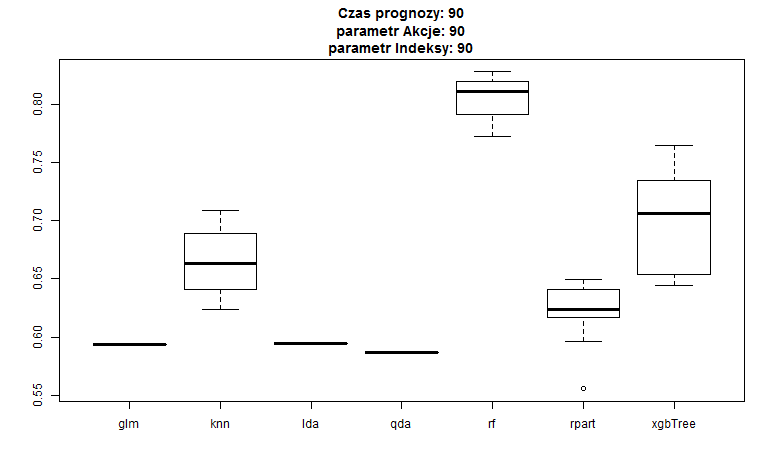
\includegraphics[scale=0.5]{./rys010b}
\caption{Skuteczność różnych modeli bazowych na zbiorze treningowym dla 90-dniowej prognozy. \textit{Źródło:} Opracowanie własne}\label{rys010b}
\end{figure}


Posiadając nauczone modele bazowe jesteśmy także w stanie dokonać predykcji używając zbioru testowego i na tej podstawie ocenić zdolność predykcyjną wybranych algorytmów. Ponadto możemy zastosować opisane w rozdziale 2 reguły kombinacyjne. Do stworzenia kombinacji prawdopodobieństw użyto średniej, średniej ważonej, mediany, reguły maksimum i minimum. W każdym z tych przypadków ustalono próg odcięcia przynależności do danej klasy na 0,5. Dla średniej ważonej wagi zostały ustalone na podstawie skuteczności najlepszego algorytmu na zbiorze treningowym (im wyższa skuteczność, tym większa waga danej metody). Ponadto po przypisaniu klas na podstawie wartości progu odcięcia dla kolejnych algorytmów, dokonano głosowania większościowego. Porównanie skuteczności klasyfikatorów połączonych za pomocą reguł kombinacyjnych dla wybranych okien prognozy przedstawia tabela~\ref{tab009}.


\begin{table}[ht] 
\caption{Skuteczność reguł kombinowanych na zbiorze testowym dla 1-dniowej prognozy. \textit{Źródło:} Opracowanie własne}
\label{tab009}
\centering
\begin{tabular}{lc}
  \hline
Reguła & Skuteczność\\
  \hline
Srednia & 0,53816\\
Srednia wazona & 0,53774\\
Mediana & 0,53563\\
Majority vote & 0,53469\\
Regula maksimum & 0,53357\\
Regula minimum & 0,51875\\
  \hline
\end{tabular}
\end{table}

Poza zastosowaniem reguł kombinacyjnych użyto także prawdopodobieństw otrzymanych ze zbioru treningowego do kontaminacji modeli. Szczegółowiej, użyto regresji logistycznej w celu znalezienia liniowej kombinacji między wynikami poszczególnych modeli, a logarytmem szans. Dzięki takiemu podejściu, jesteśmy także w stanie ocenić na podstawie oszacowanych współczynników, czy dana metoda okazała się statystycznie istotna przy objaśnianiu logarytmu ze stosunku prawdopodobieństwa wzrostu do prawdopodobieństwa porażki. Przykładowe wyniki oszacowania kontaminacji modeli za pomocą regresji logistycznej znajdują się w tabeli~\ref{tab010}. Widać, że dla tego konkretnego przykładu nieistotne okazały się 3 modele bazowe (LDA, QDA oraz drzewo decyzyjne CART). Największy wpływ na objaśnianie zmiennej celu miał algorytm lasów losowych oraz XGBoost. W ich przypadku zwiększenie prawdopodobieństwa przynależności do danej klasy zwiększało w największym stopniu szanse na poprawną klasyfikację danej obserwacji.

\begin{table}[ht] 
\caption{Oszacowania współczynników regresji logistycznej dla 20-dniowej prognozy. \textit{Źródło:} Opracowanie własne}
\label{tab010}
\centering
\begin{tabular}{lcc}
  \hline
Model bazowy & Oszacowanie & P-value\\
   \hline
(Stała) & -2,462873603 & 1,25E-34\\
knn & 0,202309196 & 1,24E-06\\
random forest & 2,955782123 & 1,60E-65\\
glm & -1,15526303 & 0,762180787\\
lda & 0,77033854 & 0,840574998\\
qda & 0,004974356 & 0,938834128\\
cart & -0,4638331 & 0,000892988\\
xgboost & 1,868288936 & 1,64E-70\\
bagging cart & 0,70153708 & 3,17E-10\\
  \hline
\end{tabular}
\end{table}


Ponadto użyto również algorytmu XGBoost w celu znalezienie nieliniowych zależności między konkretnymi algorytmami. Podobnie jak w przypadku bazowych modeli użyto 3-krotnej walidacji krzyżowej, aby dobrać odpowiednie parametry algorytmu. 

\section{Wyniki}

Wyniki przedstawiające skuteczność 5 najlepszych modeli dla wszystkich wariantów okna prognozy przedstawione są w tabelach~\ref{tab011}, \ref{tab012}, \ref{tab013}, \ref{tab014}, \ref{tab015}, oraz~\ref{tab016}. Widać, że dla każdej sytuacji użycie kontaminacji modeli było w stanie poprawić zdolność predykcyjną pojedynczych algorytmów. Co ciekawe, w 5 na 6 przypadków najskuteczniejszym modelem okazał się model wykorzystujący regresję liniową do połączenia działania wielu algorytmów uczenia maszynowego. Należy jednak zwrócić uwagę, że poprawa skuteczności dzięki zastosowaniu stackingu nie jest diametralna i poprawia wynik w stosunku do najlepszych pojedynczych klasyfikatorów o 3-4 miejsca po przecinku.

Ponadto możemy zauważyć, że wraz z wydłużaniem okna prognozy modele są w stanie lepiej rozpoznawać wzorce ukryte w danych (ok. 54\% skuteczności dla 1-dniowej prognozy do ok. 93\% w przypadku prognozy 90\%). Na podstawie wyników jesteśmy także w stanie stwierdzić, że najlepiej w objaśnianiu sprawdzały się predyktory zawierające informacje o dłuższym okresie (np. zmienność liczona na podstawie 270 obserwacji). Niższa skuteczność prognoz na 270 dni wynika właśnie z nie uwzględnienia w roli zmiennych objaśniających parametrów o wysokim interwale.


\begin{table}[ht]
\caption{Skuteczność 5 najlepszych modeli dla 1-dniowej prognozy. \textit{Źródło:} Opracowanie własne}
\label{tab011}
\centering
\begin{tabular}{rrlr}
  \hline
Stock\_param & Index\_param & Method & Accuracy \\ 
  \hline
      90 &       90 & GLM stacking & 0.5488900 \\ 
        10 &       10 & xgbTree & 0.5475431 \\ 
        20 &       20 & GLM stacking & 0.5463603 \\ 
        20 &       20 & xgbTree & 0.5460783 \\ 
       270 &      270 & GLM stacking & 0.5454640 \\ 
   \hline
\end{tabular}
\end{table}


\begin{table}[ht]
\caption{Skuteczność 5 najlepszych modeli dla 5-dniowej prognozy. \textit{Źródło:} Opracowanie własne}
\label{tab012}
\centering
\begin{tabular}{rrlr}
  \hline
Stock\_param & Index\_param & Method & Accuracy \\ 
  \hline
     270 &      270 & GLM stacking & 0.7069825 \\ 
       270 &      270 & rf & 0.7066708 \\ 
       270 &      270 & XGBTREE stacking & 0.7050603 \\ 
        90 &       90 & GLM stacking & 0.6864366 \\ 
        90 &       90 & XGBTREE stacking & 0.6858082 \\ 
   \hline
\end{tabular}
\end{table}


\begin{table}[ht]
\caption{Skuteczność 5 najlepszych modeli dla 10-dniowej prognozy. \textit{Źródło:} Opracowanie własne}
\label{tab013}
\centering
\begin{tabular}{rrlr}
  \hline
Stock\_param & Index\_param & Method & Accuracy \\ 
  \hline
     270 &      270 & GLM stacking & 0.7905040 \\ 
       270 &      270 & XGBTREE stacking & 0.7903998 \\ 
       270 &      270 & rf & 0.7887339 \\ 
       270 &      270 & treebag & 0.7667118 \\ 
       270 &      270 & Srednia wazona & 0.7560392 \\ 
   \hline
\end{tabular}
\end{table}


\begin{table}[ht]
\caption{Skuteczność 5 najlepszych modeli dla 20-dniowej prognozy. \textit{Źródło:} Opracowanie własne}
\label{tab014}
\centering
\begin{tabular}{rrlr}
  \hline
Stock\_param & Index\_param & Method & Accuracy \\ 
  \hline
     270 &      270 & GLM stacking & 0.8585769 \\ 
       270 &      270 & XGBTREE stacking & 0.8574790 \\ 
       270 &      270 & rf & 0.8530873 \\ 
       270 &      270 & treebag & 0.8376118 \\ 
       270 &      270 & Srednia wazona & 0.8206723 \\ 
   \hline
\end{tabular}
\end{table}


\begin{table}[ht]
\caption{Skuteczność 5 najlepszych modeli dla 90-dniowej prognozy. \textit{Źródło:} Opracowanie własne}
\label{tab015}
\centering
\begin{tabular}{rrlr}
  \hline
Stock\_param & Index\_param & Method & Accuracy \\ 
  \hline
     270 &      270 & GLM stacking & 0.9336457 \\ 
       270 &      270 & XGBTREE stacking & 0.9328378 \\ 
       270 &      270 & rf & 0.9281521 \\ 
       270 &      270 & treebag & 0.9230355 \\ 
       270 &      270 & adaboost & 0.9131793 \\ 
   \hline
\end{tabular}
\end{table}


\begin{table}[ht]
\caption{Skuteczność 5 najlepszych modeli dla 270-dniowej prognozy. \textit{Źródło:} Opracowanie własne}
\label{tab016}
\centering
\begin{tabular}{rrlr}
  \hline
Stock\_param & Index\_param & Method & Accuracy \\ 
  \hline
      20 &       20 & XGBTREE stacking & 0.7770807 \\ 
        20 &       20 & GLM stacking & 0.7754601 \\ 
        20 &       20 & rf & 0.7650042 \\ 
        20 &       20 & treebag & 0.7618151 \\ 
        20 &       20 & adaboost & 0.7318068 \\ 
   \hline
\end{tabular}
\end{table}

Istotną kwestią jest także, jakich modeli bazowych używamy. Rysunek~\ref{rys011} oraz~\ref{rys012} przedstawiają macierze korelacji pomiędzy prawdopodobieństwami przynależności do konkretnej klasy na zbiorze treningowym dla różnych metod, dla 1- oraz 90-dniowej prognozy. Porównując te macierze z wynikami algorytmów w tabeli~\ref{tab011} oraz~\ref{tab015} stwierdzamy, iż kontaminacja modeli przynosi lepsze rezultaty w sytuacjach kiedy uda zbudować się modele o jak największej różnorodności (niska korelacja predykcji).


\begin{figure}
\centering
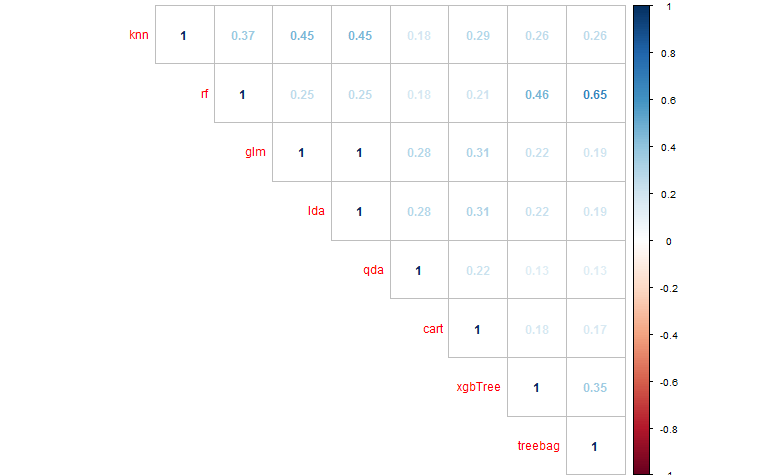
\includegraphics[scale=0.5]{./rys011}
\caption{Macierz korelacji między prawdopodobieństwami ze zbioru treningowego dla 1-dniowej prognozy. \textit{Źródło:} Opracowanie własne}\label{rys011}
\end{figure}


\begin{figure}
\centering
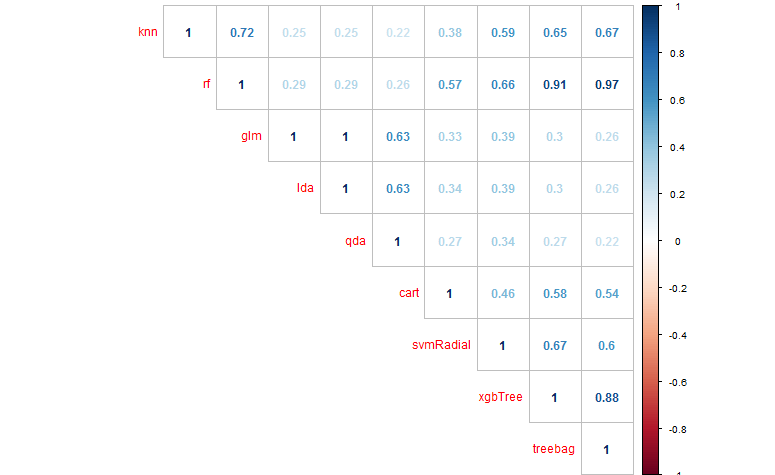
\includegraphics[scale=0.5]{./rys012}
\caption{Macierz korelacji między prawdopodobieństwami ze zbioru treningowego dla 90-dniowej prognozy. \textit{Źródło:} Opracowanie własne}\label{rys012}
\end{figure}


Widząc wysoką skuteczność metody kontaminacji modeli za pomocą regresji logistycznej możemy użyć oszacowanych za jej pomocą współczynników i dzięki temu stwierdzić, które modele bazowe są istotne w prognozowaniu kierunku zmian cen na warszawskim parkiecie. Tabele~\ref{tab017}, \ref{tab018}, \ref{tab019}, \ref{tab020}, \ref{tab021} oraz~\ref{tab022} zawierają wyniki oszacowań wraz z p-value dla testu istotności poszczególnych parametrów.

Algorytm lasów losowych oraz XGBoost okazały się być najczęściej istotnymi niezależnie od długości okresu prognozy (odpowiednio 5 na 6 oraz 4 na 6 razy statystycznie istotne dla każdej kombinacji parametrów zmiennych objaśniających). Najrzadziej statystycznie istotne okazały się być metody niewymagające parametryzacji, tzn. liniowa oraz kwadratowa analiza dyskryminacyjna, a także regresja logistyczna. Co ciekawe, algorytm k-najbliższych sąsiadów dla 1-dniowej prognozy nie był ani razu statystycznie istotny, jednak wydłużając okres prognozy stawał się coraz częściej ważny przy objaśnianiu zmiennej celu.


\begin{table}[ht]
\caption{Oszacowania współczynników dla kontaminacji modeli za pomocą regresji logistycznej dla 1-dniowej prognozy. \textit{Źródło:} Opracowanie własne}
\label{tab017}
\centering
\resizebox{\textwidth}{!}{\begin{tabular}{lllllllllllll}
  \hline
Akcje.parametr & Indeks.parametr & X.Intercept. & knn & rf & glm & lda & qda & cart & svmRadial & xgbTree & svmLinear & treebag \\ 
  \hline
10 & 10 & \makecell{1.20619059 \\ (0.74347)} & \makecell{-0.01156692 \\ (0.97278)} & \makecell{0.3835078 \\ (0.02761)} & \makecell{15.6915196 \\ (0.59822)} & \makecell{-17.89245418 \\ (0.55062)} & \makecell{-0.05328324 \\ (0.37613)} & \makecell{-0.36509476 \\ (0.36459)} & \makecell{2.4321843 \\ (0.00163)} & \makecell{1.55469165 \\ (0)} & \makecell{-3.84231455 \\ (0.56794)} & \makecell{0.05448397 \\ (0.58418)} \\ 
  10 & 5 & \makecell{-0.05964688 \\ (0.98761)} & \makecell{-0.14031482 \\ (0.6855)} & \makecell{0.17520398 \\ (0.31366)} & \makecell{-1.43355133 \\ (0.96973)} & \makecell{-0.28432581 \\ (0.99402)} & \makecell{-0.04408237 \\ (0.47646)} & \makecell{-0.92885392 \\ (0.08672)} & \makecell{0.63616818 \\ (0.53711)} & \makecell{2.37185795 \\ (0)} & \makecell{-0.23003104 \\ (0.97368)} & \makecell{0.20177175 \\ (0.04088)} \\ 
  20 & 20 & \makecell{-1.51309243 \\ (0.00016)} & \makecell{-0.40635703 \\ (0.22493)} & \makecell{0.70466587 \\ (0.00014)} & \makecell{-281.75738968 \\ (0.05607)} & \makecell{283.68270241 \\ (0.05479)} & \makecell{-0.03407748 \\ (0.75383)} & \makecell{-0.21355203 \\ (0.5397)} &  & \makecell{1.11632499 \\ (0)} &  & \makecell{-0.02735662 \\ (0.79136)} \\ 
  20 & 5 & \makecell{2.7497093 \\ (0.15383)} & \makecell{-0.22199407 \\ (0.38586)} & \makecell{0.67383199 \\ (0.00045)} & \makecell{-107.84703629 \\ (0.57911)} & \makecell{108.47864162 \\ (0.57753)} & \makecell{-0.0887174 \\ (0.42171)} & \makecell{-0.30608899 \\ (0.01494)} & \makecell{1.21634166 \\ (0.36767)} & \makecell{1.44388301 \\ (0)} & \makecell{-8.28086286 \\ (0.01031)} & \makecell{-0.02482768 \\ (0.80393)} \\ 
  270 & 270 & \makecell{-2.24512081 \\ (0)} & \makecell{-0.51761916 \\ (0.12565)} & \makecell{0.25608907 \\ (0.12344)} & \makecell{-310.7057671 \\ (0.32338)} & \makecell{313.6314176 \\ (0.32003)} & \makecell{-0.06619817 \\ (0.59093)} & \makecell{0.12592559 \\ (0.46094)} &  & \makecell{1.55700255 \\ (0)} &  & \makecell{0.18852935 \\ (0.09842)} \\ 
  90 & 5 & \makecell{-0.003288555 \\ (0.99669)} & \makecell{-0.205034029 \\ (0.55559)} & \makecell{0.441539148 \\ (0.01894)} & \makecell{-148.103927901 \\ (0.0468)} & \makecell{150.029552752 \\ (0.04455)} & \makecell{-0.038888242 \\ (0.79713)} & \makecell{-0.55597478 \\ (0.24705)} & \makecell{-0.065486211 \\ (0.93459)} & \makecell{1.913621111 \\ (0)} & \makecell{-3.270772754 \\ (0.02174)} & \makecell{0.079967876 \\ (0.43672)} \\ 
  90 & 90 & \makecell{-1.92709878 \\ (0)} & \makecell{0.36705 \\ (0.2711)} & \makecell{0.48246264 \\ (0.00602)} & \makecell{-148.04034117 \\ (0.07926)} & \makecell{149.9565638 \\ (0.07614)} & \makecell{0.04232682 \\ (0.76251)} & \makecell{0.19580343 \\ (0.54059)} &  & \makecell{1.07988695 \\ (0)} &  & \makecell{-0.22182987 \\ (0.03887)} \\ 
   \hline
\end{tabular}}
\end{table}

\begin{table}[ht]
\caption{Oszacowania współczynników dla kontaminacji modeli za pomocą regresji logistycznej dla 5-dniowej prognozy. \textit{Źródło:} Opracowanie własne}
\label{tab018}
\centering
\resizebox{\textwidth}{!}{\begin{tabular}{lllllllllll}
  \hline
Akcje.parametr & Indeks.parametr & X.Intercept. & knn & rf & glm & lda & qda & cart & xgbTree & treebag \\ 
  \hline
10 & 10 & \makecell{-2.02645517 \\ (0)} & \makecell{0.18942452 \\ (0)} & \makecell{1.89163525 \\ (0)} & \makecell{-74.55551709 \\ (0.2008)} & \makecell{74.99681631 \\ (0.19856)} & \makecell{-0.04246307 \\ (0.69915)} & \makecell{-0.02348873 \\ (0.84624)} & \makecell{1.3419623 \\ (0)} & \makecell{0.26008622 \\ (0.01865)} \\ 
  20 & 20 & \makecell{-2.2120666 \\ (0)} & \makecell{0.255747 \\ (0)} & \makecell{4.136979 \\ (0)} & \makecell{-562.1774615 \\ (0.07098)} & \makecell{561.7808176 \\ (0.07123)} & \makecell{-0.1202727 \\ (0.196)} & \makecell{-0.2325291 \\ (0.04187)} & \makecell{0.7098627 \\ (0)} & \makecell{0.1077488 \\ (0.3426)} \\ 
  270 & 270 & \makecell{-3.1980488 \\ (0)} & \makecell{0.1353781 \\ (0.00675)} & \makecell{6.3265746 \\ (0)} & \makecell{-100.4987674 \\ (0.57056)} & \makecell{99.751647 \\ (0.57416)} & \makecell{-0.2096565 \\ (0.12257)} & \makecell{-0.2752274 \\ (0.00334)} & \makecell{0.2452171 \\ (0.02669)} & \makecell{0.8706743 \\ (0)} \\ 
  5 & 5 & \makecell{-1.86566462 \\ (0)} & \makecell{0.24637923 \\ (0.25727)} & \makecell{1.7256913 \\ (0)} & \makecell{9.46992686 \\ (0.64849)} & \makecell{-9.34798712 \\ (0.65429)} & \makecell{-0.01125403 \\ (0.89246)} & \makecell{0.32785565 \\ (0.02931)} & \makecell{1.21301061 \\ (0)} & \makecell{0.13143715 \\ (0.24052)} \\ 
  90 & 90 & \makecell{-2.8122732 \\ (0)} & \makecell{0.4285093 \\ (0)} & \makecell{5.594175 \\ (0)} & \makecell{-759.4254814 \\ (0.04149)} & \makecell{759.1310664 \\ (0.04167)} & \makecell{-0.2561818 \\ (0.09538)} & \makecell{-0.4618022 \\ (0.00013)} & \makecell{0.1121704 \\ (0.29804)} & \makecell{0.4806514 \\ (0.00006)} \\ 
   \hline
\end{tabular}}
\end{table}

\begin{table}[ht]
\caption{Oszacowania współczynników dla kontaminacji modeli za pomocą regresji logistycznej dla 10-dniowej prognozy. \textit{Źródło:} Opracowanie własne}
\label{tab019}
\centering
\resizebox{\textwidth}{!}{\begin{tabular}{lllllllllll}
  \hline
Akcje.parametr & Indeks.parametr & X.Intercept. & knn & rf & glm & lda & qda & cart & xgbTree & treebag \\ 
  \hline
10 & 10 & \makecell{-2.168803128 \\ (0)} & \makecell{0.197178759 \\ (0.00016)} & \makecell{2.478167557 \\ (0)} & \makecell{7.589826048 \\ (0.52675)} & \makecell{-7.669398846 \\ (0.52508)} & \makecell{-0.009147207 \\ (0.93844)} & \makecell{-0.214621962 \\ (0.22348)} & \makecell{1.469622708 \\ (0)} & \makecell{0.497013482 \\ (0.00001)} \\ 
  20 & 20 & \makecell{-2.5140012 \\ (0)} & \makecell{0.2417425 \\ (0)} & \makecell{4.4940017 \\ (0)} & \makecell{-116.942224 \\ (0.08174)} & \makecell{116.1492685 \\ (0.08398)} & \makecell{-0.1177922 \\ (0.12098)} & \makecell{-0.2498562 \\ (0.00469)} & \makecell{1.0144255 \\ (0)} & \makecell{0.4443491 \\ (0.00012)} \\ 
  270 & 270 & \makecell{-3.5802807 \\ (0)} & \makecell{0.07037176 \\ (0.18852)} & \makecell{7.7746966 \\ (0)} & \makecell{-110.18281388 \\ (0.00065)} & \makecell{109.37723893 \\ (0.00076)} & \makecell{-0.15498641 \\ (0.36463)} & \makecell{-1.05348292 \\ (0)} & \makecell{0.05134418 \\ (0.65826)} & \makecell{1.23351699 \\ (0)} \\ 
  5 & 5 & \makecell{-2.11466814 \\ (0)} & \makecell{-0.77277248 \\ (0.00987)} & \makecell{2.7676505 \\ (0)} & \makecell{-14.8972334 \\ (0.11077)} & \makecell{15.47591226 \\ (0.102)} & \makecell{-0.07516808 \\ (0.54636)} & \makecell{-0.02767074 \\ (0.82495)} & \makecell{1.54475458 \\ (0)} & \makecell{0.21821627 \\ (0.05073)} \\ 
  90 & 90 & \makecell{-2.680297 \\ (0)} & \makecell{0.5516231 \\ (0)} & \makecell{6.490049 \\ (0)} & \makecell{-156.1272379 \\ (0.4205)} & \makecell{154.8190918 \\ (0.42496)} & \makecell{-0.4342501 \\ (0.00083)} & \makecell{-1.124837 \\ (0)} & \makecell{0.2512017 \\ (0.02186)} & \makecell{0.9731173 \\ (0)} \\ 
   \hline
\end{tabular}}
\end{table}

\begin{table}[ht]
\caption{Oszacowania współczynników dla kontaminacji modeli za pomocą regresji logistycznej dla 20-dniowej prognozy. \textit{Źródło:} Opracowanie własne}
\label{tab020}
\centering
\resizebox{\textwidth}{!}{\begin{tabular}{lllllllllll}
  \hline
Akcje.parametr & Indeks.parametr & X.Intercept. & knn & rf & glm & lda & qda & cart & xgbTree & treebag \\ 
  \hline
10 & 10 & \makecell{-2.462873603 \\ (0)} & \makecell{0.202309196 \\ (0)} & \makecell{2.955782123 \\ (0)} & \makecell{-1.15526303 \\ (0.76218)} & \makecell{0.77033854 \\ (0.84057)} & \makecell{0.004974356 \\ (0.93883)} & \makecell{-0.4638331 \\ (0.00089)} & \makecell{1.868288936 \\ (0)} & \makecell{0.70153708 \\ (0)} \\ 
  20 & 20 & \makecell{-2.7258137 \\ (0)} & \makecell{0.2959409 \\ (0)} & \makecell{4.8667114 \\ (0)} & \makecell{17.8261517 \\ (0.62282)} & \makecell{-18.9679919 \\ (0.60118)} & \makecell{-0.1559925 \\ (0.02441)} & \makecell{-0.6078713 \\ (0)} & \makecell{1.0659384 \\ (0)} & \makecell{1.136473 \\ (0)} \\ 
  270 & 270 & \makecell{-4.05067611 \\ (0)} & \makecell{0.09601793 \\ (0.11234)} & \makecell{8.66277253 \\ (0)} & \makecell{-157.30749436 \\ (0.16269)} & \makecell{156.76919165 \\ (0.16653)} & \makecell{-0.42537995 \\ (0.01006)} & \makecell{-1.22431116 \\ (0)} & \makecell{-0.42280959 \\ (0.00066)} & \makecell{1.95758748 \\ (0)} \\ 
  5 & 5 & \makecell{-2.03906469 \\ (0)} & \makecell{-1.21396918 \\ (0.00002)} & \makecell{2.71316069 \\ (0)} & \makecell{9.45558751 \\ (0.10773)} & \makecell{-9.10760579 \\ (0.1278)} & \makecell{-0.08713636 \\ (0.22766)} & \makecell{0.07149239 \\ (0.4647)} & \makecell{1.71071635 \\ (0)} & \makecell{0.56446345 \\ (0)} \\ 
  90 & 90 & \makecell{-3.601831 \\ (0)} & \makecell{0.5243417 \\ (0)} & \makecell{7.829519 \\ (0)} & \makecell{-428.504216 \\ (0.07602)} & \makecell{426.7426598 \\ (0.07787)} & \makecell{-0.3320983 \\ (0.0168)} & \makecell{-1.0480651 \\ (0)} & \makecell{0.2734387 \\ (0.0176)} & \makecell{1.724957 \\ (0)} \\ 
   \hline
\end{tabular}}
\end{table}

\begin{table}[ht]
\caption{Oszacowania współczynników dla kontaminacji modeli za pomocą regresji logistycznej dla 90-dniowej prognozy. \textit{Źródło:} Opracowanie własne}
\label{tab021}
\centering
\resizebox{\textwidth}{!}{\begin{tabular}{llllllllllll}
  \hline
Akcje.parametr & Indeks.parametr & X.Intercept. & knn & rf & glm & lda & qda & cart & xgbTree & treebag & svmRadial \\ 
  \hline
10 & 10 & \makecell{-2.42291867 \\ (0)} & \makecell{-0.71192764 \\ (0.00044)} & \makecell{2.57449946 \\ (0)} & \makecell{1.19895937 \\ (0.71339)} & \makecell{-1.72144029 \\ (0.60422)} & \makecell{-0.11430528 \\ (0.23189)} & \makecell{-0.05414481 \\ (0.61937)} & \makecell{1.90950964 \\ (0)} & \makecell{1.78847912 \\ (0)} &  \\ 
  20 & 20 & \makecell{-3.0809249 \\ (0)} & \makecell{0.1917764 \\ (0.00003)} & \makecell{4.9000342 \\ (0)} & \makecell{5.9872109 \\ (0.2704)} & \makecell{-7.3764658 \\ (0.18119)} & \makecell{-0.2153326 \\ (0.02426)} & \makecell{-0.6168348 \\ (0)} & \makecell{1.4991398 \\ (0)} & \makecell{1.7589378 \\ (0)} &  \\ 
  270 & 270 & \makecell{-3.9662568 \\ (0)} & \makecell{0.3475114 \\ (0.00002)} & \makecell{9.3451727 \\ (0)} & \makecell{28.3094153 \\ (0.2585)} & \makecell{-29.6311064 \\ (0.24347)} & \makecell{-0.1351509 \\ (0.49049)} & \makecell{-1.5500536 \\ (0)} & \makecell{-0.8213695 \\ (0)} & \makecell{2.5903943 \\ (0)} & \makecell{-0.5184306 \\ (0.00022)} \\ 
  5 & 5 & \makecell{-2.25589992 \\ (0)} & \makecell{-1.02188957 \\ (0.00024)} & \makecell{2.04877432 \\ (0)} & \makecell{-3.23643825 \\ (0.87555)} & \makecell{3.20507207 \\ (0.87747)} & \makecell{-0.17330356 \\ (0.06444)} & \makecell{0.00295194 \\ (0.97675)} & \makecell{2.14486687 \\ (0)} & \makecell{1.54667974 \\ (0)} &  \\ 
  90 & 90 & \makecell{-3.4472615 \\ (0)} & \makecell{0.4281653 \\ (0)} & \makecell{6.6460362 \\ (0)} & \makecell{16.8965748 \\ (0.14047)} & \makecell{-19.4648088 \\ (0.09247)} & \makecell{-0.2938664 \\ (0.06061)} & \makecell{-1.8453591 \\ (0)} & \makecell{0.772683 \\ (0)} & \makecell{3.7274991 \\ (0)} &  \\ 
   \hline
\end{tabular}}
\end{table}

\begin{table}[ht]
\caption{Oszacowania współczynników dla kontaminacji modeli za pomocą regresji logistycznej dla 270-dniowej prognozy. \textit{Źródło:} Opracowanie własne}
\label{tab022}
\centering
\resizebox{\textwidth}{!}{\begin{tabular}{llllllllllll}
  \hline
Akcje.parametr & Indeks.parametr & X.Intercept. & knn & rf & glm & lda & qda & cart & svmRadial & xgbTree & treebag \\ 
  \hline
10 & 10 & \makecell{-2.5663918 \\ (0)} & \makecell{-1.9786984 \\ (0)} & \makecell{2.9006559 \\ (0)} & \makecell{3.5854674 \\ (0.45632)} & \makecell{-4.1207306 \\ (0.39582)} & \makecell{0.1181847 \\ (0.16231)} & \makecell{-0.379682 \\ (0.00019)} & \makecell{1.2853422 \\ (0)} & \makecell{1.7100019 \\ (0)} & \makecell{1.9753513 \\ (0)} \\ 
  20 & 20 & \makecell{-3.41715593 \\ (0)} & \makecell{-0.01753883 \\ (0.79176)} & \makecell{5.06277867 \\ (0)} & \makecell{-144.32195574 \\ (0.02948)} & \makecell{143.44981794 \\ (0.03087)} & \makecell{-0.18893279 \\ (0.0378)} & \makecell{-1.43047839 \\ (0)} & \makecell{0.58358349 \\ (0.00003)} & \makecell{1.29888911 \\ (0)} & \makecell{2.24024768 \\ (0)} \\ 
  5 & 5 & \makecell{-2.4541568 \\ (0)} & \makecell{-2.1476071 \\ (0)} & \makecell{2.3964296 \\ (0)} & \makecell{-200.7451837 \\ (0.10581)} & \makecell{200.5214982 \\ (0.10703)} & \makecell{0.2422971 \\ (0.00676)} & \makecell{-0.3003428 \\ (0.0037)} & \makecell{1.0514087 \\ (0)} & \makecell{2.1920198 \\ (0)} & \makecell{1.571505 \\ (0)} \\ 
   \hline
\end{tabular}}
\end{table}



\chapter{Wnioski końcowe}

Podsumowując otrzymane wyniki możemy stwierdzić, 




\clearpage
\addcontentsline{toc}{chapter}{Bibliografia}
\begin{thebibliography}{99}
\setlength{\itemsep}{0pt}%

\bibitem[Adebiyi i Adewumi(2014)]{adebiyi2014} Adebiyi A., A.~Adewumi(2014), Stock Price Prediction Using the ARIMA Model

\bibitem[Ajaykumar et al.~(2016)]{ajaykumar2016} Ajaykumar R., A.~Gupta, PSN.~Merchant(2016), Automated Lane Detection by K-means Clustering: A Machine Learning Approach 

\bibitem[Allen i Gorton(1992)]{allen1992} Allen F., G.~Gorton(1992), Stock price manipulation, market microstructure and asymmetric information

\bibitem[Arowolo(2013)]{arowolo2013} Arowolo W.B.(2013), Predicting Stock Prices Return Using Garch Model, \textit{International Journal of Engineering and Science}

\bibitem[Basu(1977)]{basu1977} Basu S.(1977), Investment Performance of Common Stocks in Relation to their Price-Earnings Ratios: A Test of The Efficiency Market Hypothesis

\bibitem[Bell i Koren(2007)]{bell2007} Bell R.M., Y.~Koren(2007), Lessons from the Netflix prize challange

\bibitem[Belson(1959)]{belson1959} Belson W.(1959), Matching and Prediction on the Principle of Biological Classification

\bibitem[Bennett i Lanning(2007)]{bennett2007} Bennett J., S.~Lanning(2007), The Netflix Prize

\bibitem[Bontempi et al.~(2012)]{bontempi2012} Bontempi G., S.B.~Taieb, Y.-A. L.~Borgne(2012), Machine Learning Strategies for Time Series Forecasting

\bibitem[Bottou et al.~(1994)]{bottou1994} Bottou L., C.~Cortes, J.S.~Denker, H.~Drucker, I.~Guyon, L.D.~Jackel, Y.~LeCun, U.A.~Muller, E.~Sackinger, P.~Simard, V.~Vapnik(1994), Comparison of classifier methods: a case study in handwritten digit recognition

\bibitem[Bouman i Jacobsen(2002)]{bouman2002} Bouman S., B.~Jacobsen(2002), The Haloween indicato:r Sell in May and go Away an even bigger puzzle

\bibitem[Breiman(1996)]{breiman1996} Breiman L.(1996), Bagging predictors

\bibitem[Breiman(1996b)]{breiman1996b} Breiman L.(1996), Stacked Regressions

\bibitem[Breiman(2001)]{breiman2001} Breiman L.(2001), Random Forests

\bibitem[Ciregan et al.~(2012)]{ciregan2012} Ciregan D., U.~Meier, J.~Schmidhuber(2012), Multi-column deep neural networks for image classification

\bibitem[Citak(2007)]{citak2007} Citak L.(2007), The Effect of Beta Coefficients on Extreme Single-Day Stock Returns: The Case of Istanbul Stock Exchange

\bibitem[Cox(1958)]{cox1958} Cox D.R.(1958), The regression analysis of binary sequences(with discussion)

\bibitem[De Gooijer i Hyndman(2006)]{degooijer2006} De Gooijer J.G., R.J.~Hyndman(2006), 25 years of time series forecasting

\bibitem[Dietterich(2000)]{dietterich2000} Dietrich T.G.(2000), Ensemble methods in Machine Learning

\bibitem[Ferreira i Santa-Clara(2008)]{ferreira2008} Ferreira M., P.~Santa-Clara(2008), Forecasting Stock Market Returns: The Sum of the Parts is More than the Whole

\bibitem[Fisher(1936)]{fisher1936} Fisher R.A.(1936), The Use of Multiple Measurements in Taxonomic Problems

\bibitem[Frank(2000)]{frank2000} Frank E.(2000), Pruning Decision Trees and Lists

\bibitem[Freund i Schapire(1997)]{freund1997} Freund Y., R.E.~Schapire(1997), A decision-theoretic generalization of on-line learning and an application to boosting

\bibitem[Friedman(1999)]{friedman1999} Friedman J.H.(1999), Stochastic Gradient Boosting

\bibitem[Friedman(2001)]{friedman2001} Friedman J.H.(2001), Greedy function approximation: A gradient boosting machine

\bibitem[Garcia-Almanza i Tsang(2006)]{almanza2006} Garcia-Almanza A., E.~Tsang(2006), Forecasting stock prices using Genetic Programming and Chance Discovery

\bibitem[Granger(1992)]{granger1992} Granger C.(1992), Forecasting stock market prices: Lessons for forecasters, \textit{International Journal of Forecasting}

\bibitem[Hastie et al.~(2009)]{hastie2009} Hastie T., R.~Tibshirani, J.~Friedman(2009), The Elements of Statistical Learning

\bibitem[He i Garcia(2009)]{he2009} He H., E.A.~Garcia(2009), Learning from imbalanced data

\bibitem[Hinton et al.~(2012)]{hinton2012} Hinton G., L.~Deng, D.~Tu, G.E.~Dahl(2012), Deep Neural Networks for Acoustic Modeling in Speech Recognition: The Shared Views of Four Research Groups

\bibitem[Ho(1995)]{ho1995} Ho T.(1995), Random Decision Trees

\bibitem[Hodges(1983)]{hodges1983} Hodges A.(1983), Alan Turing: The Enigma

\bibitem[Hoffmann(1990)]{hoffmann1990} Hoffmann A.G.(1990) , General Limitations on Machine Learning

\bibitem[Hyafil i Rivest(1976)]{hyafil1976} Hyafil L., R.L.~Rivest(1976), Constructing Optimal Binary Decision Trees Is NP-Complete

\bibitem[Indyk i Motwani(1998)]{indyk1998} Indyk P., R.~Motwani(1998), Approximate nearest neighbors: towards removing the curse of dimensionality

\bibitem[Jacobsen i Zhang(2013)]{jacobsen2013} Jacobsen B., C.~Zhang(2013), Are Monthly Seasonals Real? A Three Century Perspective, \textit{Review of Finance}

\bibitem[Jahrer et al.~(2010)]{jahrer2010} Jahrer M., A.~Toscher, R.~Legenstein(2010), Combining predictions for accurate recommender systems

\bibitem[Jegadeesh i Titman(1993)]{jegadeesh1993} Jegadeesh N., S.~Titman(1993), Returns to Buying Winners and Selling Losers: Implications for Stock Market Efficiency, \textit{Journal of Finance}

\bibitem[Jiang(2012)]{jiang2012} Jiang W.(2012), Using the GARCH model to analyze and predict the different stock markets

\bibitem[Kara i Baykan(2011)]{kara2011} Kara Y., M.~Baykan(2011), Predicting direction of stock price index movement using artificial neural networks and support vector machines: The sample of the Istanbul Stock Exchange, \textit{Expert Systems with Applications}

\bibitem[Kass(1980)]{kass1980} Kass G.V.(1980), An Exploratory Technique for Investigating Large Quantities of Categorical Data

\bibitem[Kim i Loh(2001)]{kim2001} Kim H., W.-Y.~Loh(2001), Classification trees with unbiased multiway splits

\bibitem[Kim(2003)]{kim2003} Kim K.(2003), Financial time series forecasting using support vector machines, \textit{Neurocomputing}

\bibitem[Kleinberg(1996)]{kleinberg1996} Kleinberg E.(1996), An Overtraining-Resistant Stochastic Modeling Method for Pattern Recognition

\bibitem[Kleinberg(2000)]{kleinberg2000} Kleinberg E.(2000), On the Algorithmic Implementation of Stochastic Discrimination

\bibitem[Kohavi(1995)]{kohavi1995} Kohavi R.(1995), A Study of Cross-Validation and Bootstrap for Accuracy Estimation and Model Selection

\bibitem[Kursa i Rudnicki(2010)]{kursa2010} Kursa M.B., W.R.~Rudnicki(2010), Feature Selection with the Boruta Package, \textit{Journal of Statistical Software}

\bibitem[Kwiatkowski(1992)]{kwiatkowski1992} Kwiatkowski D.(1992), Testing the null hypothesis of stationarity against the alternative of a unit root: How sure are we that economic time series have a unit root?

\bibitem[Lin i Kernighan(1973)]{lin1973} Lin S., B.W.~Kernighan(1973), An Effective Heuristic Algorithm for the Traveling-Salesman Problem 

\bibitem[Loh i Shih(1997)]{loh1997} Loh W.-Y., Y.-S.~Shih(1997), Split selection methods for classification trees

\bibitem[Long i Servedio(2010)]{long2010} Long P.M., R.A.~Servedio(2010), Random classification noise defeats all convex potential boosters

\bibitem[Mackenzie(2009)]{mackenzie2009} Mackenzie M.(2009), High-frequency trading under scrutiny, \textit{Financial Times}

\bibitem[Madge(2015)]{madge2015} Madge S.(2015), Predicting Stock Price Direction using Support Vector Machines 

\bibitem[Moghaddam et al.~(2016)]{moghaddam2016} Moghaddam M., M.~Moghaddam, M.~Esfandyari(2016), Stock market index prediction using artificial neural network

\bibitem[Mohan et al.~(2005)]{mohan2005} Mohan N., P.~Jha, A.K.~Laga, G.~Dutta(2005), Artificial Neural Network Models for Forecasting Stock Price Index in Bombay Stock Exchange

\bibitem[Moudrik i Neruda(2015)]{moudrik2015} Moudrik J., R.~Neruda(2015), Evolving Non-linear Stacking Ensembles for Prediction of Go Player Attributes

\bibitem[Mingers(1989)]{mingers1989} Mingers J.(1989), An Empirical Comparison of Pruning Methods for Decision Tree Induction, \textit{Machine Learning}

\bibitem[Mitchell(1977)]{mitchell1977} Mitchell T.M.(1977), Machine Learning

\bibitem[Mnih et al.~(2015)]{mnih2015} Mnih V., K.~Kavukcuoglu, D.~Silver, A.A.~Rusu, J.~Veness, M.G.~Bellemare, A.~Graves, M.~Riedmiller, A.K.~Fidjeland, G.~Ostrovski, S.~Petersen, C.~Beattie, A.~Sadik, I.~Antonoglou, H.~King, D.~Kumaran, D.~Wierstra, S.~Legg, D.~Hassabis(2015), Human-level control through deep reinforcement learning

\bibitem[Murphy(1999)]{murphy1999} Murphy J.J.(1999), Analiza techniczna rynków finansowych

\bibitem[Patel i Yalamalle(2014)]{patel2014} Patel M.B., S.R.~Yalamalle(2014), Stock Price Prediction Using Artificial Neural Network, \textit{International Journal of Innovative Research in Science, Engineering and Technology}

\bibitem[Patel et al.~(2015)]{patel2015} Patel J., S.~Shah, P.~Thakkar(2015), Predicting stock and stock price index movement using Trend Deterministic Data Preparation and Machine Learning techniques

\bibitem[Purnanandam i Swaminathan(2004)]{purnanandam2004} Purnanandam A.K., B.~Swaminathan(2004), Are IPOs Really Underpriced

\bibitem[Qu et al.~(2002)]{qu2002} Qu Y., B.-L.~Adam, Y.~Yasui, M.D.~Ward, L.H.~Cazares, P.F.~Schellhammer, Z.~Feng, O.J.~Semmes, G.L.~Wright(2002), Boosted Decision Tree Analysis of Surface-enhanced Laser Desorption/Ionization Mass Spectral Serum Profiles Discriminates Prostate Cancer from Noncancer Patients

\bibitem[Rajput i Bobde(2016)]{rajput2016} Rajput V., S.~Bobde(2016), Stock market forecasting techniques: literature survey, \textit{International Journal of Computer Science and Mobile Computing}

\bibitem[Schapire(1990)]{schapire1990} Schapire R.E.(1990), The Strength of Weak Learnability. Machine Learning

\bibitem[Shen i Jiang(2015)]{shen2015} Shen S., H.~Jiang, T.~Zhang(2015), Stock Market Forecasting Using Machine Learning Algorithms

\bibitem[Sill et al.~(2009)]{sill2009} Sill J., G.~Takacs, L.~Mackey, D.~Lin(2009), Feature-Weighted Linear Stacking

\bibitem[Sureshkumar i Elango(2011)]{sureshkumar2011} Sureshkumar K.K., N.~Elango(2011), An Efficient Approach to Forecast Indian Stock Market Price and their Performance Analysis

\bibitem[Swensen(2015)]{swensen2015} Swensen J.(2015), Investigating Use of Beta Coefficients for Stock Predictions

\bibitem[Thenmozhi i Chand(2016)]{thenmozhi2016} Thenmozhi M., G.~Chand(2016), Forecasting stock returns based on information transmission across global markets using support vector machines, \textit{Neural Computing and Applications}

\bibitem[Ting i Witten(1999)]{ting1999} Ting K.M., I.H.~Witten(1999), Issues in Stack Generalization

\bibitem[Toscher et al.~(2009)]{toscher2009} Toscher A., M.~Jahrer, R.M.~Bell(2009), The BigChaos Solution to the Netflix Grand Prize

\bibitem[Vapnik(1996)]{vapnik1996} Vapnik V.(1996), The Nature of Statistical Learning Theory

\bibitem[Wolpert(1992)]{wolpert1992} Wolpert D.H.(1992), Stacked Generalization

\bibitem[Wolpert(1996)]{wolpert1996} Wolpert D.H.(1996), The Lack of A Priori Distinctions Between Learning Algorithms

\bibitem[Wong et al.~(2003)]{wong2003} Wong W.-K., M.~Manzur, B.-K.~Chew(2003), How rewarding is technical analysis? Evidence from Singapure stock market

\bibitem[Xu(2014)]{xu2014} Xu S.(2014), Stock Price Forecasting Using Information from Yahoo Finance and Google Trend

\bibitem[Zhang(2009)]{zhang2009} Zhang J.(2009), Applying Time Series Analysis Builds Stock Price Forecast Model, \textit{Modern Applied Science}

\end{thebibliography}

\clearpage
\addcontentsline{toc}{chapter}{Spis rysunków}
\listoffigures

\clearpage
\listoftables
\addcontentsline{toc}{chapter}{Spis tabel}

\appendix
\chapter*{Kody źródłowe}
\addcontentsline{toc}{chapter}{Kody źródłowe}

Skrypt \textit{bazowe\_modele.R} zawierający funkcję do budowy modeli pierwszego stopnia:
\lstinputlisting{./bazowe_modele.R}

Skrypt \textit{stacking.R} zawierający funkcję do kontaminacji modeli:
\lstinputlisting{./stacking.R}

Skrypt \textit{reguly\_kombinacyjne.R} zawierający funkcję do zastosowania reguł kombinacyjnych na prawdopodobieństwach ze zbioru testowego:
\lstinputlisting{./reguly_kombinacyjne.R}

Skrypt \textit{zebranie\_wynikow.R} zawierający zastosowanie funkcji do budowy modeli bazowych, użycia reguł kombinacyjnych, kontaminacji, a także wizualizacji otrzymanych rezultatów:
\lstinputlisting{./zebranie_wynikow.R}

\clearpage

\chapter*{Streszczenie}
\addcontentsline{toc}{chapter}{Streszczenie}

Celem niniejszej pracy była poprawa skuteczności przewidywania kierunku zmian cen akcji notowanych na Giełdzie Papierów Wartościowych w Warszawie za pomocą technik klasyfikacji kombinowanej. Trudność tego zagadnienia polegała na znalezieniu rozwiązania, które będzie skuteczne niezależnie od istniejących warunków rynkowych, tak by stało się jak najbardziej uniwersalne. W celu osiągnięcia tego celu nacisk w pracy położony został na zbudowaniu różnych algorytmów uczenia maszynowego i połączenia ich w jeden model, potrafiący wykorzystywać mocne strony poszczególnych klasyfikatorów i niwelujący słabe. Zebranie wyników modeli zostało przeprowadzone za pomocą reguł kombinacyjnych bądź kontaminacji, czyli budowaniu modelu wyższego poziomu korzystając z prawdopodobieństw modeli bazowych. Uzyskane wyniki sugerowały, że użycie klasyfikacji kombinowanej, zarówno w postaci pojedynczych modeli (lasy losowe, XGBoost), jak i kontaminacji za pomocą regresji logistycznej bądź algorytmu XGBoost zmniejsza ryzyko wyboru niewłaściwej metody bądź niewłaściwych parametrów danej metody. Ponadto pokazane zostało, że wraz ze wzrostem długości okna prognozy, algorytmy uczenia maszynowego są w stanie z lepszą skutecznością przewidywać kierunek zmian cen. W każdym przypadku osiągnięta skuteczność przekraczała 50\%, co sugeruje że hipoteza rynku efektywnego dla 20 największych pod względem kapitalizacji spółek z warszawskiego parkietu  nie jest spełniona, a zatem możliwe jest wyciąganie wniosków co przyszłego ruchu na podstawie danych historycznych. Pomimo poprawy skuteczności za pomocą \textit{stackingu} w każdym rozpatrywanym przypadku, wzrost ten nie okazał się być duży (poniżej 1\%). Jako przyczynę należy wskazać tu trudność budowy modeli, które są ze sobą nisko skorelowane, a jednocześnie mają wysoką skuteczność osobno. Być może użycie innych zmiennych objaśniających, lepiej oddających strukturę rynku pozwoliłyby na budowę modeli o takiej charakterystyce. Drugim problemem była także złożoność obliczeniowa niektórych algorytmów. Ze względu na ograniczone zasoby, nie była możliwa weryfikacja wszystkich kombinacji parametrów poszczególnych algorytmów, tak aby stworzyć jak najszerszą bazę dostępnych modeli.





\end{document}

              
            